\documentclass{article}
\LARGE
% Language setting
% Replace `english' with e.g. `spanish' to change the document language
\usepackage[english]{babel}

% Set page size and margins
% Replace `letterpaper' with `a4paper' for UK/EU standard size
\usepackage[letterpaper,top=2cm,bottom=2cm,left=3cm,right=3cm,marginparwidth=1.75cm]{geometry}


\usepackage{tikz}
\usetikzlibrary{shapes.geometric, arrows}
\tikzstyle{startstop} = [rectangle, rounded corners, minimum width=3cm, minimum height=1cm,text centered, draw=black, fill=red!30]
\tikzstyle{io} = [trapezium, trapezium left angle=70, trapezium right angle=110, minimum width=3cm, minimum height=1cm, text centered, draw=black, fill=blue!30]
\tikzstyle{process} = [rectangle, minimum width=3cm, minimum height=1cm, text centered, draw=black, fill=orange!30]
\tikzstyle{decision} = [diamond, minimum width=3cm, minimum height=1cm, text centered, draw=black, fill=green!30]
\tikzstyle{arrow} = [thick,->,>=stealth]




\pgfdeclarelayer{bg}
\pgfsetlayers{bg,main}

% Useful packages
\usepackage{amsmath}
\usepackage{amsfonts}
\usepackage{graphicx}
\usepackage[colorlinks=true, allcolors=cyan]{hyperref}
\numberwithin{equation}{section}
\usepackage{graphicx,wrapfig,lipsum,subfigure,sidecap,epsfig}
\usepackage{caption}
\usepackage{cancel}
%\usepackage{graphicx,subfigure,sidecap,epsfig} % Rouslan's subfig package
\usepackage{soul}
%\usepackage[colorlinks=true,linkcolor=red]{hyperref}%
\usepackage{mathtools}
\usepackage{eqparbox}
\usepackage{float} % \figure{}[H] IN PLACE VIEW
\usepackage[capitalize]{cleveref} % smart references in one bracket
\usepackage{hyperref}

%
% CREF rules
% Equation(s)
\crefformat{equation}{#2Eq. (#1)#3}
\crefrangeformat{equation}{#3Eqs. (#1)#4 to #5(#2)#6}
\crefmultiformat{equation}{#2Eqs. (#1)#3}{ and #2(#1)#3}{, #2(#1)#3}{ and #2(#1)#3}
\crefrangemultiformat{equation}{#3Eqs. ((#1))#4 to #5((#2))#6}{ and #3(#1)#4 to #5(#2)#6}{, #3(#1)#4 to #5(#2)#6}{ and #3(#1)#4 to #5(#2)#6}
% Plural eqn
\crefformat{pluralequation}{#2Eqs.~(#1)#3}
% System
\crefformat{system}{#2Sys.~(#1)#3}
\crefrangeformat{system}{#3Sys. (#1)#4 to #5(#2)#6}
\crefmultiformat{system}{#2Sys. (#1)#3}{ and #2(#1)#3}{, #2(#1)#3}{ and #2(#1)#3}
\crefrangemultiformat{system}{#3Sys. ((#1))#4 to #5((#2))#6}{ and #3(#1)#4 to #5(#2)#6}{, #3(#1)#4 to #5(#2)#6}{ and #3(#1)#4 to #5(#2)#6}
% Boundary conditions
\crefformat{bc}{#2BC (#1)#3}
\crefrangeformat{bc}{#3BCs (#1)#4 to #5(#2)#6}
\crefmultiformat{bc}{#2BCs (#1)#3}{ and #2(#1)#3}{, #2(#1)#3}{ and #2(#1)#3}
\crefrangemultiformat{bc}{#3BCs ((#1))#4 to #5((#2))#6}{ and #3(#1)#4 to #5(#2)#6}{, #3(#1)#4 to #5(#2)#6}{ and #3(#1)#4 to #5(#2)#6}
% Steps
\crefformat{step}{#2Step (#1)#3}
\crefrangeformat{step}{#3Steps (#1)#4 to #5(#2)#6}
\crefmultiformat{step}{#2Steps (#1)#3}{ and #2(#1)#3}{, #2(#1)#3}{ and #2(#1)#3}
\crefrangemultiformat{step}{#3Steps ((#1))#4 to #5((#2))#6}{ and #3(#1)#4 to #5(#2)#6}{, #3(#1)#4 to #5(#2)#6}{ and #3(#1)#4 to #5(#2)#6}



%\usepackage[sortcites=true]{biblatex} % biblatex DOEST WORK WITH LIVE TYPESETTER
\usepackage[nocompress]{cite}
%\bibliographystyle{ieeetr} % trash style mess up the order in bib

\graphicspath{{figures/}}


%%% Todos
\newcommand{\todo}[1]{\vspace{5 mm}\par \noindent
\marginpar{\textsc{\tiny \hspace{0.5cm} ToDo}} \framebox{\begin{minipage}[c]{0.95
\textwidth} \small \tt #1 \end{minipage}}\vspace{5 mm}\par}



\title{Discrete stream function method \\ for the incompressible Navier-Stokes equations with travelling wave boundary conditions past a flat plate}
\author{Rauan}

\begin{document}
\maketitle

\begin{abstract}
The goal of these notes is to present the detailed overview of discrete stream function method for solving incompressible Navier-Stokes equations with travelling wave boundary conditions past a flat plate. We will discuss in detail the scheme formulation, transient and spatial discretizations. Special attention will be paid to the boundary conditions and their implementation. After studying these notes one must get a coherent picture of the application of discrete stream function method to incompressible flows and be able to implement the scheme in code.
\end{abstract}

\tableofcontents

\section{Introduction}\label{sec:introduction}

In these notes we will be concerned with the discretization of the Navier-Stokes equations describing the flow of an incompressible fluid:
\begin{subequations}
\label[pluralequation]{eqs:NSE}
\begin{align}
\label{eqn:momentum-intro}
\frac{\partial \boldsymbol{v}}{\partial t} + \boldsymbol{v} \cdot \nabla \boldsymbol{v} &= -\nabla p + \epsilon \nabla \cdot \nabla \boldsymbol{v} \\
\label{eqn:continuity}
\nabla \cdot \boldsymbol{v} &= 0,
\end{align}
\end{subequations}
which are written here in the non-dimensional form, i.e. $\epsilon \equiv Re^{-1}$ for brevity; also $\boldsymbol{v}$ is the velocity and $p$ pressure fields. Since both are necessarily functions of time $t$ and space $\boldsymbol{x}$, their discretization will be denoted by $f^{n}_{i}$, where $n$ is the time level $t^{n}$ and $i$ is the \textit{mesh} point $\boldsymbol{x}_{i}$: for example, in the $x$-direction the interval $x_{i} < x < x_{i+1}$ is referred to as the \textit{cell} of the mesh. The cell centre corresponds to $x_{i+\frac{1}{2}}$. The mesh points $x_{i}$ and cell centres $x_{i \pm \frac{1}{2}}$ can be regarded as two overlapping interpenetrating meshes, which together are said to constitute a \textit{staggered} mesh as illustrated in figure~\ref{fig:grid-MAC}. When designing a finite difference or finite volume scheme, we have to choose whether to use the same or different sets of grid points for velocity and pressure. The obvious choice seems to have a single set of points, at which all the variables and all the equations are discretized. Such a grid
has the name of a \textit{collocated} or \textit{regular} grid. Albeit simple and easy in operation, the collocated grids were out of favor for a long time because of their tendency to generate spurious oscillations in the solution (cf. \S 10.2 in \cite{Zikanov:2010}) and hence staggered grids are used since the work of Harlow and Welch \cite{Harlow:1965} introducing the marker-and-cell (MAC) method, cf. figure~\ref{fig:grid-MAC}.
\begin{figure}[H]
\centering
  \subfigure[MAC]{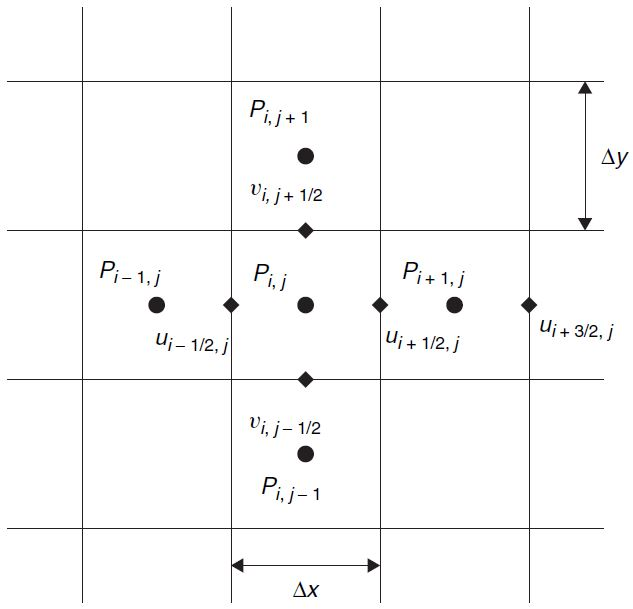
\includegraphics[height=0.295\textwidth]{grid-MAC.jpg} \label{fig:grid-MAC}} \quad
  \subfigure[general]{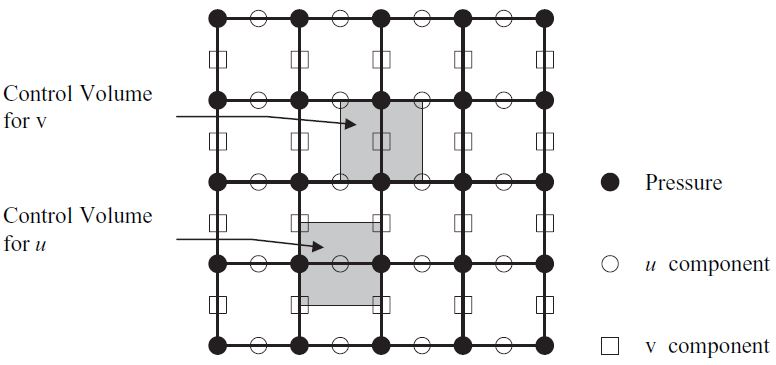
\includegraphics[height=0.295\textwidth]{grid-staggered.jpg} \label{fig:grid-staggered}}
\caption{\small Staggered grid.}
\end{figure}


The staggered arrangement increases complexity of a scheme. Programming becomes more difficult, since it requires accounting for three (or four in the three-dimensional case) indexing systems. Interpolations must be used to compute nonlinear terms of momentum equations. Further complications arise when the grid is nonuniform. All these difficulties, however, can be relatively easily handled in computations with structured grids such as those shown in figure~\ref{fig:grid-staggered}. For this reason and because of the benefit of removing the splitting problem, the staggered arrangement was by far the most popular choice during early years of CFD. The difficulties of handling a staggered arrangement increase significantly when unstructured grids are used. When such grids started to
be broadly applied in general-purpose codes in recent years, collocated arrangements returned to favor. This area of CFD is still evolving. We only mention that methods have been developed to cure the splitting problem leading to pressure oscillations, but the cure is not ideal and leads to extra complexities at the implementation level.

In numerical terms, the problem \cref{eqs:NSE} can be formulated as follows: given the solution $p^{n}$, $\boldsymbol{v}^{n}$ at the previous time layer $t^{n}$, find the next time-layer pressure $p^{n+1}$ and velocity $\boldsymbol{v}^{n+1}$ such that they together satisfy the momentum equation, and the velocity is divergence-free $\nabla \cdot \boldsymbol{v}^{n+1} = 0$ and satisfies the boundary conditions.

A conspicuous feature of \cref{eqs:NSE} is that pressure $p$ is not determined by a time-evolution equation, but rather is implicitly defined by the incompressibility \cref{eqn:continuity}, which plays the role of a constraint that the velocity field $\boldsymbol{v}$ must satisfy. The pressure instantaneously adapts to the evolving velocity field in such a way as to satisfy that constraint. This is reflected in the fact that $p$ satisfies a Poisson equation, which can be derived by taking the divergence of \cref{eqn:momentum-intro} and combining the result with \cref{eqn:continuity}. From the mathematical viewpoint, this means that the incompressible flow equations have some features of an elliptic system. We can say that the equations are of the mixed hyperbolic (convective terms), parabolic (viscous terms), and elliptic (pressure and incompressibility) type. The elliptic nature of the pressure solution has a physical meaning. It shows that, in an incompressible flow, the pressure field in the entire flow domain adjusts instantaneously to any, however localized, perturbation. This is in perfect agreement with the fact that weak perturbations, for example sound waves, propagate at infinite speed in incompressible fluids.

Given the Poisson equation for $p$, it may replace the continuity \cref{eqn:continuity} and its solution can in principle be substituted back into \cref{eqn:momentum-intro} to obtain an evolution equation for the velocity field alone. Alternatively, the pressure can be immediately eliminated by taking the $\mathrm{curl}$ of momentum \cref{eqn:momentum-intro}, which leads to the vorticity-stream function formulation of incompressible flow. Formal manipulations of this type are useful for various theoretical purposes, but experience has shown that they are rarely advantageous for computational purposes. In most situations, it is preferable to simply approximate and solve \cref{eqs:NSE} directly for the so-called \textit{primitive} variables $\boldsymbol{v}$ and $p$.

If, however, one ends up solving the Poisson equation for pressure, an interesting and important question arises as to what boundary conditions should be used for the pressure field. Such conditions are required at every point of the boundary for the Poisson problem to be well-posed. The conditions, however, do not naturally follow from the flow physics for the boundaries between fluid and solid walls, unless, of course, a full fluid-structure interaction problem is solved. Since the latter option is, in most cases, an unnecessary complication, we have to find a way to derive the pressure boundary conditions from the equations themselves.

%\section{Discrete streamfunction method}\label{sec:discrete-streamfunction}
%%%%%%%%%%%%%%%%%%%%%%%%%%%%%%%%%%%%%%%%%%%%%%%%%%%%%%%%%%%%%%%%%%%%%%
%There are a few things to add/clarify:
%1. Non-dimensionalization.
%2. BC discussion (analytic).
%3. Symmetric BC on top to be included in all operators. 
%4. Scaling of G and D operators. 
%5. Indexation change.
%%%%%%%%%%%%%%%%%%%%%%%%%%%%%%%%%%%%%%%%%%%%%%%%%%%%%%%%%%%%%%%%%%%%%%
\todo{
\begin{itemize}
%    \item \st{Non-dimensionalization.} \st{Shall we keep u component under value of 1? can multiply the freestream and inlet by 0.5 if needed.} Normalized to max value of 1.
%	\item \st{Scaling of G and D operators.} \textit{$\left(C^T\right)\left(\hat{M}\right)\left(\hat{G}\right)p=\left(C^T\right)\left(\hat{M}\right)\left(\hat{M}^{-1}{G}\right)p=C^TGp=(-DC)^Tp=0$.}
%    \item \st{Symmetric BC on top to be included in all operators.}
%    \item \st{Indexing change for equations and figures.}
    \item \st{Motivation.} Added some, where possible!
    \item \st{BC discussion (analytic).} \cite{Engquist:1977,Kourta:1987,Liu:1993,Sani:1994,Persillon:1998,Tsynkov:1998}.
    \item \st{Outlet diffusion discretization is problematic. Requested PhD thesis of Jin and Persillon through UofA library. Wrote an email to their supervisor Prof. Braza and sent a message to Persillon.} Waiting for the response form UofA library since 11th Dec. 
%    \item \st{Substitute all refs/eqrefs with smart \textbackslash cref and use one bracket for \textbackslash cite.} 
%    \item Is it ok to use "Sys. (43)" for SLAE?
%    \item \st{Time step $n$ is in superscript, however, domain dim's are $n\times m$, dimension index is in subscript.} Changed dimensions to $M\times N$
%    \item Outlet idea 1. (headache division by zero) might be using uniform grid in the direction of the flow and refine grid only vertically. Will use three-point scheme into the domain, but then matrix L becomes asymmetric. 
%	\item Outlet idea 2. Use extrapolation $\frac{\partial ^2 \boldsymbol{v}}{\partial x^2}=0$ or BC by Kourta $\frac{\partial ^2u}{\partial x^2}=0,\frac{\partial v}{\partial x	}=0$.
    \item  \st{Found this condition $\frac{\partial \boldsymbol{v}}{\partial t}+u \frac{\partial \boldsymbol{v}}{\partial x}+v \frac{\partial \boldsymbol{v}}{\partial y}-\epsilon \frac{\partial^2 \boldsymbol{v}}{\partial y^2}=0$ by G. Fournier and F. Golanski (2008, but not many citations). They claim Prandtl BL solution for advective bc $\frac{\partial \boldsymbol{v}}{\partial t} + u\frac{\partial \boldsymbol{v}}{\partial x}=0$ is wrong, while their solution matches Prandtl BL. Looks like we can express the remaining diffusive summand in terms of pressure gradient at the boundary.} Wrote an email to author, waiting for the response. 
    \item \st{Change computational domain to inner part only? Boundary values are to be determined by BC, not the momentum eq'n, contrary to Hall}\cite{Hall:1980}. Changed unknowns to inner part only. Values at the boundary are determined using BC. 
    \item \st{Check algebra of diffusion and advection for $v$ component.} 
    \item It feels like BC scheme which is consistent with inner discretization won't work, we will use Jin-Braza-Braza scheme. 
    \item Outlet BC stated early in non-dim truncated part, but discussion is much later.
    \item Continuous analogue of $C^T$ to be determined. Figured out that $C^TC=L$ and $C^TLC=L^2$. Some information of transpose of curl is in \href{https://www.math.mcgill.ca/gantumur/math248f19/vectorcalc.pdf}{Vector Calculus notes} on page 24 of \href{https://www.math.mcgill.ca/gantumur/math248f19/}{course by TSOGTGEREL GANTUMUR}, but the material is quite heavy.
    \item Repeating \cref{fig:luxx-right-first} from first try of Laplacian and \cref{fig:luxx-right} after Artificial BC discussion.
  \end{itemize}
}

\section{Problem statement}\label{sec:problem-statement-dimentional}
Let the velocity vector $\boldsymbol{v}(t,x,y)=(u(t,x,y),v(t,x,y))$ and pressure $p(t,x,y)$ be the solutions to ~\cref{eqs:NSE} on a semi-infinite domain together with boundary conditions:
\begin{subequations}
\label[pluralequation]{eqs:NSE-dsm-bl-dimensional}
\begin{align}
\label{eqn:momentum-dimensional}
\text{Momentum: }	&\frac{\partial \boldsymbol{v}}{\partial t} + \boldsymbol{v} \cdot \nabla \boldsymbol{v} = -\frac{1}{\rho}\nabla p + {\frac{\mu}{\rho}} \nabla \cdot \nabla \boldsymbol{v},\\
&\rho\text{ - density}, \mu\text{ - dynamic viscosity.}\notag\\
\label{eqn:continuity-dsm-bl}
\text{Continuity: }	& \nabla \cdot \boldsymbol{v} = 0, \\ 
					&0\leq x < \infty, 0\leq y <\infty, t\geq0.\notag\\
\label{eqn:NSE-dsm-bl-bc-freestream}
\text{Inlet and Freestream BC: } 	& \boldsymbol{v}(t,0,y)=\boldsymbol{v}(t,x,\infty)=\left(U_0 + A\cos\left( kx -\omega t + \phi_0 \right),0\right),\\
									& \{|A|<U_0,k,\omega, \phi_0\}\subset \mathbb{R}.\notag\\
\label[bc]{eqn:NSE-dsm-bl-bc-noslip}
\text{No-slip BC: } & \boldsymbol{v}(t,x,0)=(0,0). \\
%\label{eqn:NSE-dsm-bl-bc-outlet}
%\text{Outlet BC: } 	& \frac{\partial u}{\partial t}+u\frac{\partial u}{\partial x}=0\lor\left(\frac{\partial u}{\partial t}+u\frac{\partial u}{\partial x}=\epsilon \frac{\partial ^2 u}{\partial y^2}\right), \\ 
%					& v=\boldsymbol{h}(t,y)-\text{linear extrapolation},\notag\\
%					& (x=\infty),\notag\\
\text{Initial condition: } &\boldsymbol{v}(0,x,y)=(0,0) \text{ or Blasius profile.}
\end{align}
\end{subequations}



%\subsubsection{Top BC}\label{subsubsec:top-bc}

\section{Nondimensionalization}\label{sec:nondimensionalization}
In numerical computations, it is advantageous to maintain variables of comparable magnitude. This ensures that operations such as the multiplication of a large dimensional pressure variable with a small velocity are not performed. 

We will truncate the domain and normalize all equations by width $L$ and stream velocity $U_0$. After introducing the following dimensionless variables (marked with prime ${ }^{\prime}$ ):
\begin{equation*}
	x\to Lx^{\prime},  \quad 
	\boldsymbol{v}\to U_0\boldsymbol{v}^{\prime}, \quad 
	\nabla\to \frac{1}{L}\nabla^{\prime}, \quad 
%	\Delta \to \frac{1}{L^2} \Delta^{\prime},  \quad 
	p\to p^{\prime} \rho U_0^2, \quad 
	t\to \frac{L}{U_0}t^{\prime},
\end{equation*}
we obtain
\begin{equation*}
	\frac{U_0}{\frac{L}{U_0}} \frac{\partial \boldsymbol{v}^{\prime}}{\partial t^{\prime}}+U_0\boldsymbol{v}\cdot\left(\frac{1}{L} \nabla^{\prime}\right) U_0\boldsymbol{v}=-\frac{1}{\rho}\left(\frac{1}{L} \nabla^{\prime}\right){p^{\prime}\rho U^2_0}+\frac{\mu}{\rho} \left(\frac{1}{L} \nabla^{\prime}\right) \cdot\left(\frac{1}{L} \nabla^{\prime}\right) U_0\boldsymbol{v}^{\prime}.
\end{equation*}
After multiplying both sides of the equation by $\frac{L}{U_0^2}$ and introducing well-known Reynolds number 
\begin{equation*}
\operatorname{Re}=\frac{\rho L U_0}{\mu},
\end{equation*}
we obtain the non-dimensional momentum equation
\begin{equation*}
	\frac{\partial \boldsymbol{v}}{\partial t} + \boldsymbol{v} \cdot \nabla \boldsymbol{v} = -\nabla p + \frac{1}{\operatorname{Re}} \nabla \cdot \nabla \boldsymbol{v},
\end{equation*}
where prime superscript $\prime$ is suppressed for the dimensionless variables. The continuity equation is nondimensionalized in a similar manner:
\begin{equation*}
	\left(\frac{1}{L} \nabla^{\prime}\right) \cdot U_0\boldsymbol{v}^{\prime}=0\iff\nabla^{\prime} \cdot\boldsymbol{v}^{\prime}=0\implies\nabla \cdot\boldsymbol{v}=0,
\end{equation*}
where we drop prime superscripts in the last identity as well.


\section{Problem statement on truncated domain}
The initial \cref{eqs:NSE-dsm-bl-dimensional} from \cref{sec:problem-statement-dimentional} on semi-infinite domain now become a system of partial differential equations on a unit square domain 
\begin{subequations}
\label[pluralequation]{eqs:NSE-dsm-bl}
\begin{align}
\label{eqn:momentum}
\text{Momentum: }	&\frac{\partial \boldsymbol{v}}{\partial t} + \boldsymbol{v} \cdot \nabla \boldsymbol{v} = -\nabla p + \epsilon \nabla \cdot \nabla \boldsymbol{v}, \\ 
					&\epsilon = \frac{1}{\operatorname{Re}},0\leq x \leq 1, 0\leq y \leq 1, t\geq0.\notag\\
\label{eqn:continuity-dsm-bl}
\text{Continuity: }	& \nabla \cdot \boldsymbol{v} = 0, \\ 
					&0\leq x \leq 1, 0\leq y \leq 1, t\geq0. \notag\\
\label[bc]{eqn:NSE-dsm-bl-bc-freestream}
\text{Inlet and Freestream BC: } 	& \boldsymbol{v}(t,0,y)=\boldsymbol{v}(t,x,1)=\left(1 + A\cos\left( kx -\omega t + \phi_0 \right),0\right),\\
									& \{A\leq 1,k,\omega, \phi_0\}\subset \mathbb{R}.\notag\\
\label[bc]{eqn:NSE-dsm-bl-bc-noslip}
\text{No-slip BC: } & \boldsymbol{v}(t,x,0)=(0,0). \\
\label[bc]{eqn:NSE-dsm-bl-bc-outlet}
\text{Outlet BC: } 	&\frac{\partial \boldsymbol{v}}{\partial t}+u\frac{\partial \boldsymbol{v}}{\partial x}-\epsilon \frac{\partial^2 \boldsymbol{v}}{\partial y^2}=0,\text{ discussed in \cref{sec:artificial-bc}}, \\ 
					& (x=1).\notag\\
\text{Initial condition: } &\boldsymbol{v}(0,x,y)=(0,0)\text{ or Blasius profile}.
\end{align}
\end{subequations}

\section{Domain discretization}\label{sec:dsm-domain}
Following the nondimensionalization of the governing equations, we now turn our attention to the process of domain discretization. This crucial step involves dividing the computational domain into discrete elements, allowing us to compute variables and their derivatives on a finite set of points called grid. Consider discretizing the area into $M$ intervals horizontally and $N$ intervals vertically forming a mesh of rectangular cells. To enhance memory access it is recommended to organize the data using vectors instead of matrices. The reason is that accessing memory using a single index $i$ works faster than double $i,j$ in most programming languages. In this section, however, for the sake of simplicity, we use two indices $i,j$ (column and row as in Harlow and Welch~\cite{Harlow:1965}) to represent coordinates on the grid.

\begin{figure}[H] % here, bottom, top
  \centering{
  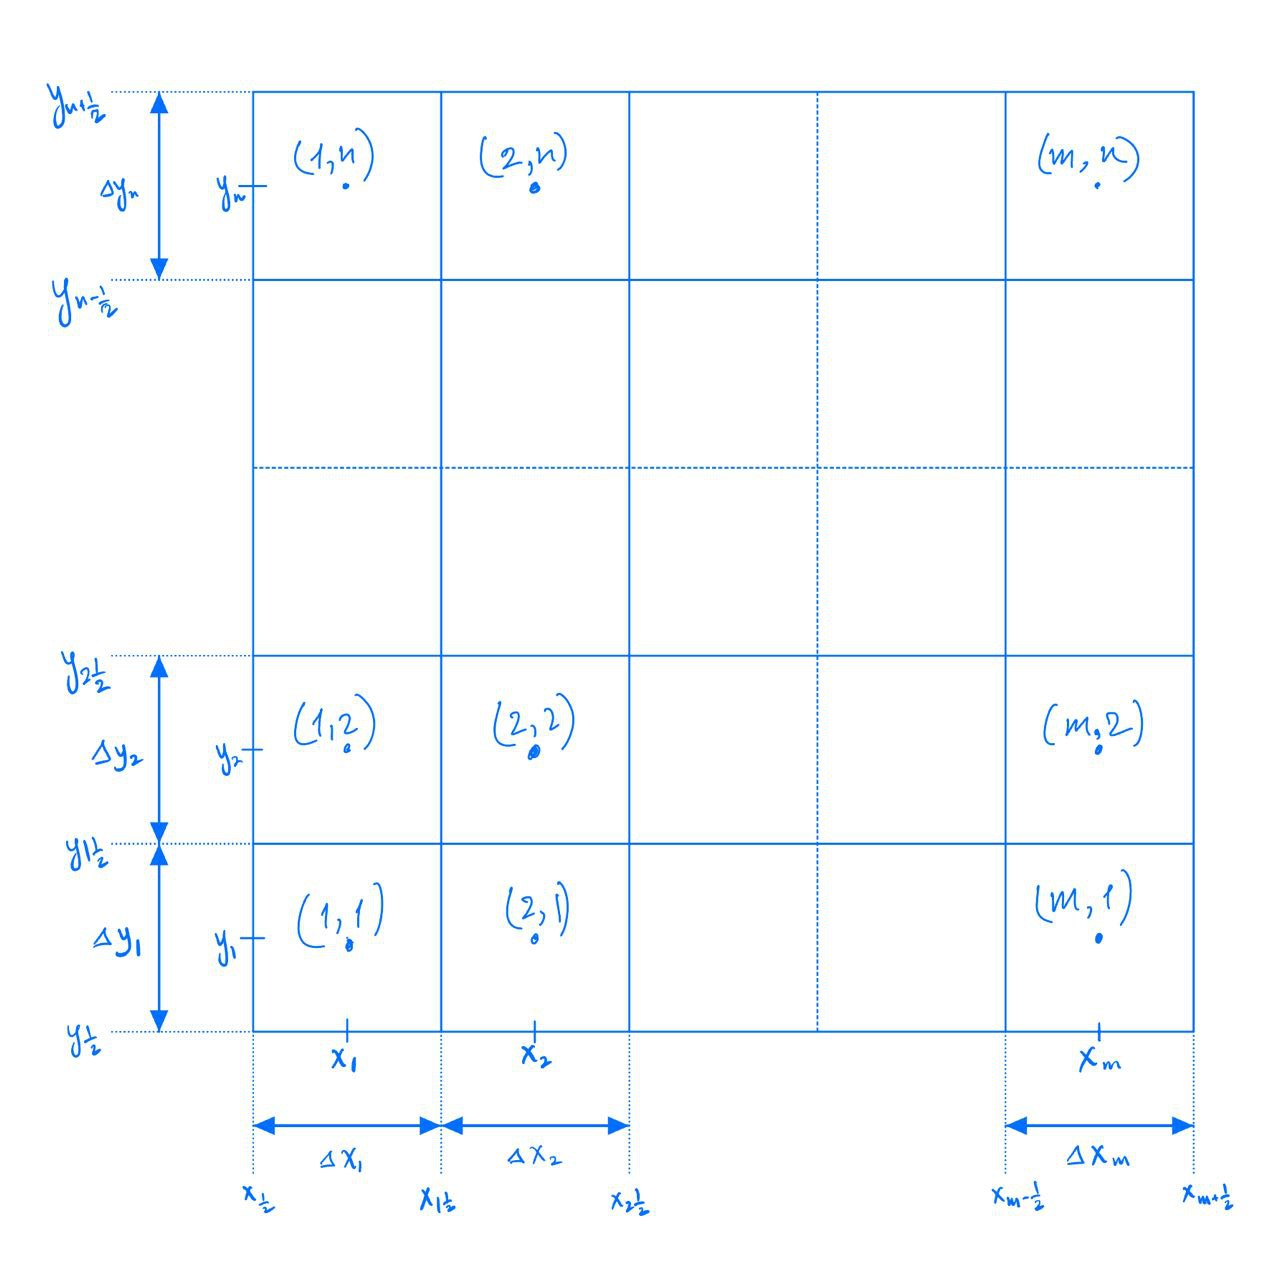
\includegraphics[width=0.45\paperwidth]{grid-bl}
  }
  \caption{Domain discretization}\label{bl-domain-discretization}
\end{figure}

To eliminate the necessity of solving an additional equation for pressure we will be using a staggered grid arrangement. 
Moreover, the pressure gradients can be evaluated directly using central differences on such grids. 
This calculation does not require any interpolation on staggered grids, furthermore, it is computationally cheaper and simple. 
Details are discussed in \cref{subsec:divergence,subsec:gradient,sec:nullspace-method}. 
The $u$ velocity components are stored at the centres of vertically oriented faces, while the values of $v$ are stored at the centres of horizontal ones. 

The number of unknown components inside the domain (excluding boundaries) is $M(N-1)$ for $v$ and $(M-1)N$ for $u$. In \cref{eqn:NSE-dsm-bl-bc-outlet}, the values of $u$ for the outlet are not explicitly defined. To address this, we will express the values on the boundary using \cref{eqn:NSE-dsm-bl-bc-outlet} in terms of data from inner part of the domain. These arrays for $u$ and $v$ are then concatenated into a single vector $\boldsymbol{v}$ of size $M(N-1)+(M-1)N$.

Increasing the accuracy closer to the wall and the outlet does look advantageous, hence, we will refine the grid using the standard ratio rule $\Delta x_{i+1}=k_x\Delta x_i,\Delta y_{j+1}=k_y\Delta y_j$ with constants $k_x,k_y$ close to the value of $1$. Grid indexation starts at $(x_{\frac{1}{2}},y_{\frac{1}{2}})=(0,0)$ and ends at $(x_{M+\frac{1}{2}},y_{N+\frac{1}{2}})=(1,1)$. The intervals $\Delta x, \Delta y$ have the same indexation as the corresponding cells they belong to. 

%%%%%%%%%%%%%%%%%%%%%%%%%%%%%%%%%%%%%%%%%%%%%%%%%%%%%%%%
\section{Discrete operators}

This subsection focuses on the specific operators used in the discretization of \cref{eqs:NSE-dsm-bl}, providing the mathematical tools necessary to transform these continuous equations into a form that can be solved numerically.

Denote discrete spatial operators as
\begin{enumerate}
	\item[$\hat{L}$]:  Laplacian.
	\item[$\hat{G}$]: Gradient.
	\item[$\hat{D}$]: Divergence.
	\item[$\mathbf{\hat{H}}$]: Non-linear advective terms.
\end{enumerate}
Then initial system of \cref{eqs:NSE-dsm-bl} can be approximated using such operators as
\begin{equation}\label[system]{eqn:nse-matrix}
            \begin{bmatrix}
                  \mathbf{I} && 0 \\ 
                  0 && 0
            \end{bmatrix}
            \frac{\partial }{\partial t} 
            \begin{pmatrix}
                  \boldsymbol{v} \\ 
                  p
            \end{pmatrix}
            =
            \begin{bmatrix}
                  \hat{L} && - \hat{G} \\ 
                  -\hat{D} && 0
            \end{bmatrix}
            \begin{bmatrix}
                  \boldsymbol{v} \\
                  p
            \end{bmatrix}
            +
            \begin{pmatrix}
                  -\mathbf{\hat{H}}(\boldsymbol{v})\\
                  0
            \end{pmatrix} + \text{bc}_{\boldsymbol{v},p},
        \end{equation}
where boundary conditions are in terms of pressure and velocity. In the following subsections, each of the discrete operators is described individually. 

%%%%%%%%%%%%%%%%%%%%%%%%%%%%%%%%%%%%%%%%%%%%%%%%%%%%%%%%%%%
%\subsubsection{Transient terms}\label{subsec:transient}
Attack \cref{eqn:nse-matrix} with the following schemes as in Colonius~\cite{Colonius:2008} (superscript denotes the time step):
\begin{enumerate}
	\item[\textbf{Viscous}] - Implicit trapezoidal - Crank Nicholson scheme (second-order method in time).  
%	\begin{equation}\label{eqn:crank-nicholson}
%		\frac{\boldsymbol{v}^{n+1}-\boldsymbol{v}^n}{\Delta t}=\frac{1}{2}\left[F^{n+1}+F^n\right],
%	\end{equation}
	\begin{equation}\label{eqn:viscous-crank-nicholson}
  		\hat{L}\boldsymbol{v}=\frac{1}{2}\left(\hat{L}\boldsymbol{v}^{n+1}+\hat{L}\boldsymbol{v}^n\right)
	\end{equation}

	\item[\textbf{Nonlinear}] - Explicit Adams-Bashforth (second-order method in time).
%	\begin{equation}\label{eqn:adams-bashforth}
%		\frac{\boldsymbol{v}^{n+1}-\boldsymbol{v}^{n}}{\Delta t} = \frac{3}{2}F^{n} - \frac{1}{2}F^{n-1}.
%	\end{equation}
	\begin{equation}\label{eqn:nonlinear-adams-bashforth}
		\mathbf{\hat{H}}(\boldsymbol{v}) = \frac{3}{2}\mathbf{\hat{H}}(\boldsymbol{v}^{n}) - \frac{1}{2}\mathbf{\hat{H}}(\boldsymbol{v})^{n-1}.
	\end{equation}

	\item[\textbf{Pressure}] - Implicit Euler, though the pressure variable will be later eliminated in the algorithm (first-order method in time). 
%	\begin{equation}\label{eqn:implicit-euler} 
%		\frac{\boldsymbol{v}^{n+1}-\boldsymbol{v}^{n}}{\Delta t} = F^{n+1}.
%	\end{equation}
	\begin{equation}\label{eqn:pressure-implicit-euler} 
		\hat{G}p = \hat{G}p^{n+1}.
	\end{equation}
\end{enumerate}

The above schemes result in the following time-discretized system:
\begin{equation}\label[system]{eqn:NSE-dsm-bl-system-schemes}
	\begin{bmatrix}
		\frac{1}{\Delta t}\mathbf{I}-\frac{1}{2}\hat{L} & \hat{G} \\
		\hat{D} & 0
	\end{bmatrix}
	\begin{pmatrix}
		\boldsymbol{v}^{n+1} \\ 
		p^{n+1}
	\end{pmatrix}
	=
	\begin{pmatrix}
		\left[\frac{1}{\Delta t}\mathbf{I}-\frac{1}{2}\hat{L}\right] \boldsymbol{v}^n - \left[\frac{3}{2}\hat{\mathbf{H}}(\boldsymbol{v}^n) - \frac{1}{2}\hat{\mathbf{H}}(\boldsymbol{v}^{n-1})\right]\\
		0
	\end{pmatrix}
	+
	\begin{pmatrix}
		\hat{bc}_1\\
		\hat{bc}_2
	\end{pmatrix}
\end{equation}
and \cref{eqn:Jin-Braza-bc} 
\begin{equation}\label[bc]{eqn:Jin-Braza-bc-transient-consistent}
\begin{gathered}
\frac{\boldsymbol{v}^{n+1}-\boldsymbol{v}^n}{\Delta t}+\left[\frac{3}{2}{u^n}\left(\frac{\partial \boldsymbol{v}}{\partial x}\right)^{n}-\frac{1}{2}{u^{n-1}}\left(\frac{\partial \boldsymbol{v}}{\partial x}\right)^{n-1}\right] \\
=\epsilon\left[\left(\frac{\partial^2 \boldsymbol{v}}{\partial y^2}\right)^{n+1}+\left(\frac{\partial^2 \boldsymbol{v}}{\partial y^2}\right)^{n}\right],
\end{gathered}
\end{equation}
however, the results produced with such \cref{eqn:Jin-Braza-bc-transient-consistent} schemes are yet to be known and should be compared with \cref{eqn:Jin-Braza-bc-transient} from the corresponding paper of Jin-Braza\cite{Jin:1993}, which was said to be 
\begin{equation}\label[bc]{eqn:Jin-Braza-bc-transient}
\begin{gathered}
\frac{\boldsymbol{v}^{n+1}-\boldsymbol{v}^n}{\Delta t}+\frac{u^n}{2}\left[\left(\frac{\partial \boldsymbol{v}}{\partial x}\right)^{n+1}+\left(\frac{\partial \boldsymbol{v}}{\partial x}\right)^n\right] \\
=\epsilon\left(\frac{\partial^2 \boldsymbol{v}}{\partial y^2}\right)^n.
\end{gathered}
\end{equation}
We will first use discretized \cref{eqn:Jin-Braza-bc-transient} from Jin-Braza~\cite{Jin:1993} as it was shown to be stable and produced solid results. Later on we can proceed with discretized \cref{eqn:Jin-Braza-bc-transient-consistent} which is consistent with our schemes after developing the necessary techniques.

After applying the discrete operators listed in the following \cref{subsec:advection,sec:laplacian,subsec:divergence,subsec:gradient}, we rewrite \cref{eqn:NSE-dsm-bl-system-schemes}  as
\begin{equation}\label[system]{eqn:NSE-dsm-bl-system-nonint}
	\begin{bmatrix}
		\hat{A} & \hat{G} \\
		\hat{D} & 0
	\end{bmatrix}
	\begin{pmatrix}
		\boldsymbol{v}^{n+1} \\ 
		p^{n+1}
	\end{pmatrix}
	=
	\begin{pmatrix}
		\hat{r}^n \\
		0
	\end{pmatrix}
	+
	\begin{pmatrix}
		\hat{bc}_1\\
		\hat{bc}_2
	\end{pmatrix},
\end{equation}
where $\hat{r}^n$ includes viscous, non-linear and gradient terms from time steps $n,n-1$ and $\hat{bc}_i$ are explicit boundary values in terms of velocity and pressure.


%%%%%%%%%%%%%%%%%%%%%%%%%%%%%%%%%%%%%%%%%%%%%%%%%%%%%%%%%%%
\subsection{Laplacian}\label{sec:laplacian}

As per \cref{eqn:NSE-dsm-bl-system-schemes} it is required to approximate implicit viscous terms spatially. In order to obtain the discrete operator acting on a velocity vector we will rewrite Laplacian as a block matrix:
\begin{equation*}
	\hat L=
	\begin{bmatrix}
  \hat{L}^u_{xx}+\hat{L}^u_{yy} & 0 \\
  0 & \hat{L}^v_{xx}+\hat{L}^v_{yy}
\end{bmatrix}.
\end{equation*}

Each pair of the matrices $\hat{L}^u_{xx},\hat{L}^v_{xx}$ and $\hat{L}^u_{yy},\hat{L}^v_{yy}$ will be equal on a uniform, but different on non-uniform grids. These matrices are computed similarly. Below we will discuss how the Laplacian matrix is constructed at different parts of the grid.

\subsubsection{Inner part}\label{subsubsec:laplacian-inner}
The uniform grid refinement $\Delta x_{i+1}=k_x\Delta x_i,\Delta y_{j+1}=k_y\Delta y_j$ makes the order of the scheme consistent throughout the whole domain. Without loss of generality, let us show how to compute $\hat{L}^u_{xx}$. The other three matrices can be constructed in a similar manner. The power series of of $u_{i-\frac{1}{2}\pm 1,j}$ at nodes $x_{i - \frac{1}{2}\pm 1}$ with respect to $u_{i - \frac{1}{2},j}$ at node $x_{i-\frac{1}{2}}$ are
\begin{equation}\label{eqn:Taylor right} 
	u_{i-\frac{1}{2}+1,j}=u_{i-\frac{1}{2},j}+\left.\frac{\partial u}{\partial x}\right|_{i-\frac{1}{2},j}\left(x_{i-\frac{1}{2}+1}-x_{i-\frac{1}{2}}\right)+\frac{1}{2}\left.\frac{\partial^2 u}{\partial x^2}\right|_{i-\frac{1}{2},j}\left(x_{i-\frac{1}{2}+1}-x_{i-\frac{1}{2}}\right)^2+O\left(\Delta x^3\right),
\end{equation}
\begin{equation}\label{eqn:Taylor left} 
	u_{i-\frac{1}{2}-1,j}=u_{i-\frac{1}{2},j}+\left.\frac{\partial u}{\partial x}\right|_{i-\frac{1}{2},j}\left(x_{i-\frac{1}{2}-1}-x_{i-\frac{1}{2}}\right)+\frac{1}{2}\left.\frac{\partial^2 u}{\partial x^2}\right|_{i-\frac{1}{2},j}\left(x_{i-\frac{1}{2}-1}-x_{i-\frac{1}{2}}\right)^2+O\left(\Delta x^3\right).
\end{equation}
We can combine \cref{eqn:Taylor left,eqn:Taylor right} by cancelling the first derivative, which will result in
\begin{align}\label{eqn:laplacian-discretization-non-uniform-dx}
\left.\frac{\partial^2 u}{\partial x^2}\right|_{i-\frac{1}{2},j} & \approx \frac{u_{i-\frac{1}{2}+1,j}\left(x_{i-\frac{1}{2}}-x_{i-\frac{1}{2}-1}\right)-u_{i-\frac{1}{2},j}\left(x_{i-\frac{1}{2}+1}-x_{i-\frac{1}{2}-1}\right)+u_{i-\frac{1}{2}-1,j}\left(x_{i-\frac{1}{2}+1}-x_{i-\frac{1}{2}}\right)}{\left(\frac{x_{i-\frac{1}{2}+1}-x_{i-\frac{1}{2}-1}}{2}\right)\left(x_{i-\frac{1}{2}}-x_{i-\frac{1}{2}-1}\right)\left(x_{i-\frac{1}{2}+1}-x_{i-\frac{1}{2}}\right)}+O(\Delta x)\notag\\
& \approx \frac{1}{h_c h_e}u_{i-\frac{1}{2}+1} - \frac{2}{h_w h_e}u_{i-\frac{1}{2}} + \frac{1}{h_c h_w}u_{i-\frac{1}{2}-1} + O(\Delta x),
\end{align}
where $h_w=x_{i-\frac{1}{2}}-x_{i-\frac{1}{2}-1},h_c = \frac{x_{i-\frac{1}{2}+1}-x_{i-\frac{1}{2}-1}}{2}, h_e = x_{i-\frac{1}{2}+1}-x_{i-\frac{1}{2}}$ as in \cref{fig:luxx-inner}. The coefficients in front of the velocity components are then placed into the $\hat{L}^u_{xx}$ matrix. The order of this approximation becomes $2^{\text {nd }}$ for uniform grids. 

\begin{figure}[H] % here, bottom, top
  \centering{
  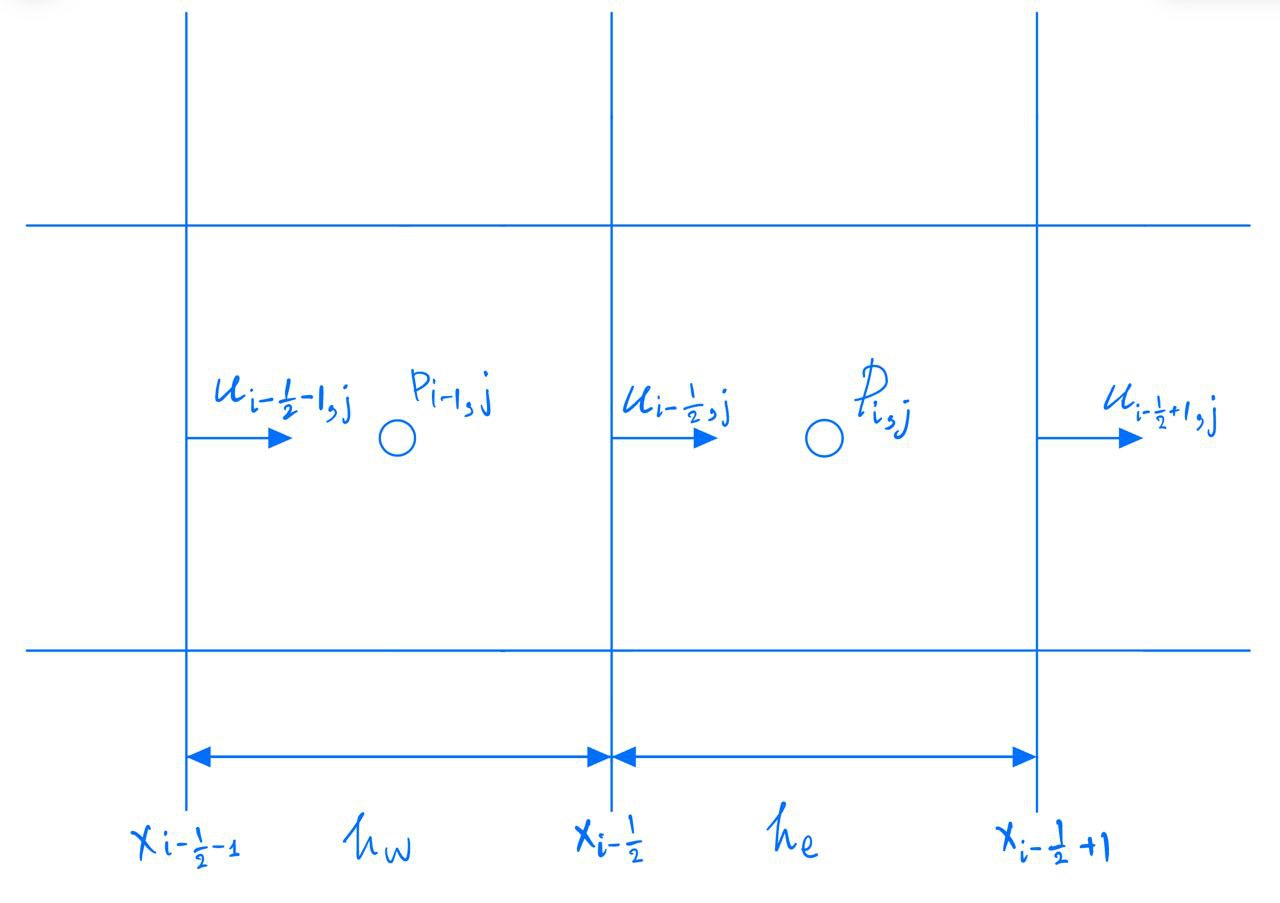
\includegraphics[width=0.45\paperwidth]{Luxx}
  }
  \caption{$\hat{L}^u_{xx}$ inner part.}\label{fig:luxx-inner}
\end{figure}
%The discretization for such grids is reduced to 
%\begin{equation}\label{eqn: second derivative uniform}
%\left(\frac{\partial^2 u}{\partial x^2}\right)_i \approx \frac{u_{i+1}-2 u_i+u_{i-1}}{(\Delta x)^2} + O(\Delta x^2).
%\end{equation}




\subsubsection{Left boundary}\label{subsubsec:laplacian-left}
The exact value on the left boundary ($u_{\frac{1}{2},j}$ in a box on \cref{fig:luxx-left}) is given as a Dirichlet boundary condition, hence, it is possible to move the corresponding terms together with the coefficients to the right-hand side of the linear system and treat the values explicitly. The values are moved to the vector $\hat{bc}_1$ on the right-hand side of \cref{eqn:NSE-dsm-bl-system-schemes}.
\begin{figure}[H] % here, bottom, top
  \centering{
  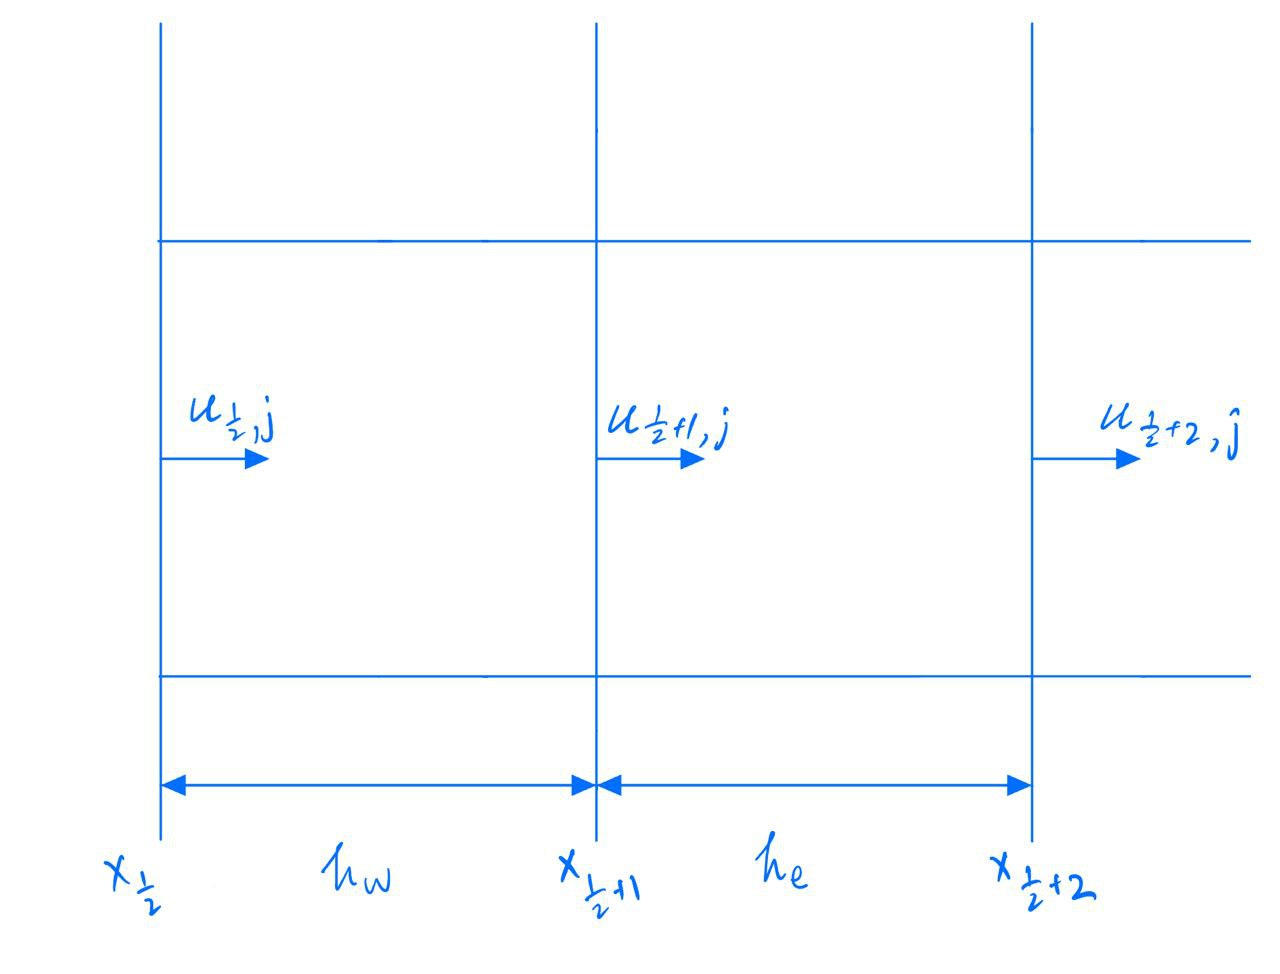
\includegraphics[width=0.55\paperwidth]{Luxx-left}
  }
  \caption{$\hat{L}^u_{xx}$ at the left boundary.}\label{fig:luxx-left}
\end{figure}

\subsubsection{Top boundary}\label{subsubsec:laplacian-top}
Most of the flow that differs much from the freestream is likely to happen closer to the wall, thus, we can incorporate symmetric boundary conditions over the top. \cref{eqn:symmetric-bc} leads to $v_{\text{top}}=0, u_{\text{top}}=u_{\text{freestream}}$, which affects only the $\hat{L}^u_{yy}$ and $\hat{L}^v_{yy}$ due to the 5-point stencil discretization. We will focus on $\hat{L}^u_{yy}$ in this part; $\hat{L}^v_{yy}$ is computed in a similar manner. 

\begin{figure}[h]
\centering{
  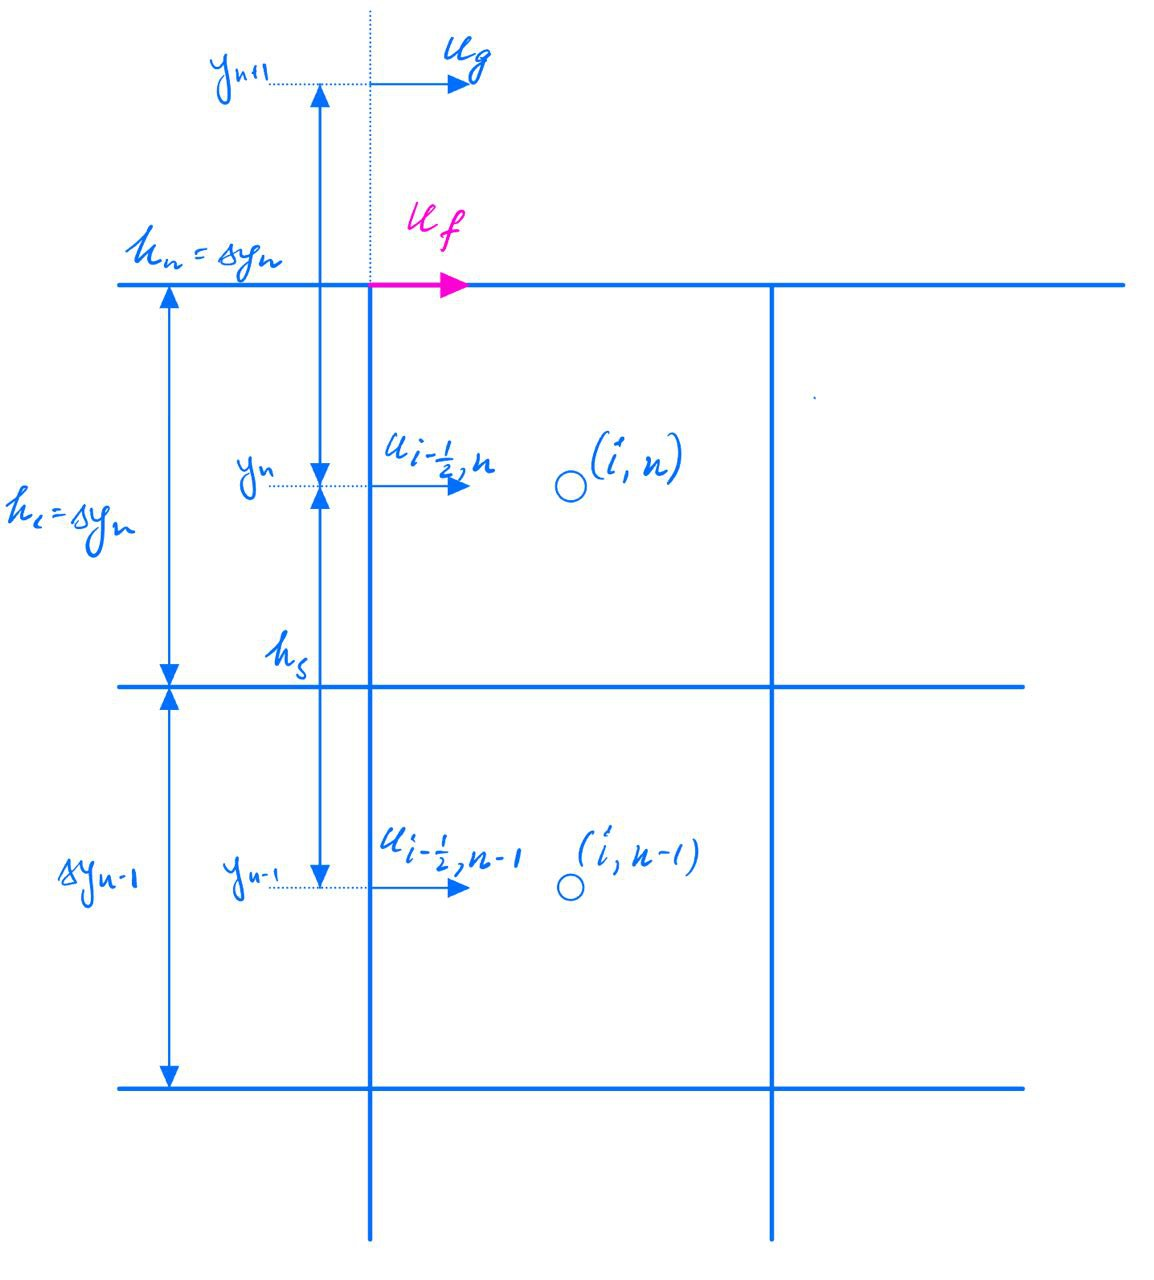
\includegraphics[width=0.45\paperwidth]{Luxx-top.jpg}
  }
  \caption{$\hat{L}^u_{yy}$ at top boundary.}\label{fig:luxx-top}
\end{figure}

Consider the neighbouring cells near the wall as in \cref{fig:luxx-top}. Resultant \cref{eqn:laplacian-discretization-non-uniform-dx}  can be written as
\begin{equation}\label{eqn:laplacian-discretization-non-uniform-dy}
\left.\frac{\partial^2 u}{\partial y^2}\right|_{i-\frac{1}{2},N}=\frac{u_g\left(h_s\right)+u_{i-\frac{1}{2},N}\left(-2 h_c\right)+u_{i-\frac{1}{2},N-1}\left(h_n\right)}{h_n h_s h_c},
\end{equation}
where $h_s=y_{n}-y_{n-1}, h_n = y_{n+1}-y_n, h_c = \frac{y_{n+1}-y_{n-1}}{2}=\frac{h_s+h_n}{2}$.

It is possible to make the order of the scheme $O(\Delta y^2)$ near the boundary as per \cref{eqn:laplacian-discretization-non-uniform-dx} if $u_g$ and $u_{i-\frac{1}{2},N-1}$ are set to be equidistant from $u_{i-\frac{1}{2},N}$.The value of $u$ along the top face is known to be freestream velocity $u_{{f}}$, interpolation of freestream velocity $u_{f} = \frac{u_g+u_{i-\frac{1}{2},N}}{2}\implies u_g=2u_{f}-u_{i-\frac{1}{2},N}$, which we can plug into \cref{eqn:laplacian-discretization-non-uniform-dy} from above to obtain
\begin{equation}
\begin{aligned}
& \left.\frac{\partial ^2 u}{\partial y^2}\right|_{i-\frac{1}{2},N}=\frac{2 u_f h_s}{h_n h_s h_c}+u_{i-\frac{1}{2},N}\left(\frac{-h_s}{h_n h_s h_c}+\frac{-2 h_c}{h_n h_s h_c}\right)+u_{i-\frac{1}{2},N-1} \frac{h_n}{u_c h_s h},\\
& \left.\frac{\partial^2 u}{\partial y^2}\right|_{i-\frac{1}{2},N}=\frac{2 u_f}{h_c h_c}+u_{i-\frac{1}{2},N}\left(\frac{-\left(2 h_c+h_s\right)}{h_c h_s h_c}\right)+u_{i-\frac{1}{2},N-1} \frac{1}{h_s h_c}, \\
& \left.\frac{\partial^2 u}{\partial y^2}\right|_{i-\frac{1}{2},N}=\frac{2 u_f}{h_c{ }^2}+u_{i-\frac{1}{2},N}\left(\frac{-\left(2 h_c+h_s\right)}{h_c^2 h_s}\right)+u_{i-\frac{1}{2},N-1} \frac{1}{h_s h_c}.
\end{aligned}
\end{equation}

The first summand from the above equation is treated explicitly, i.e. moved to the vector $\hat{bc}_1$ on the right-hand side in \cref{eqn:NSE-dsm-bl-system-schemes}, while the other two coefficients are used as elements for the $\hat{L}^u_{yy}$ matrix.

\subsubsection{Bottom boundary}\label{subsubsec:laplacian-bottom}
It is, in fact, possible to directly use the third velocity directly from the boundary. However, the order of such a scheme will then be reduced due to the large ratio of the distances between the neighbouring velocities. If, on the other hand, we introduce a ghost velocity $u_g$, we have the freedom of where to place it. Let us use \cref{eqn:laplacian-discretization-non-uniform-dx} and change the distances between velocities as in \cref{fig:luxx-bottom}, which leads to
\begin{equation}
\begin{aligned}
&\left.\frac{\partial^ 2 u}{\partial y^2}\right|_{i-\frac{1}{2},1}=u_{i-\frac{1}{2},2}\left(\frac{1}{h_n h_c}\right)+u_{i-\frac{1}{2},1}\left(\frac{-2}{h_n h_s}\right)+u_g\left(\frac{1}{h_s h_c}\right).\\
\end{aligned}
\end{equation}

\begin{figure}[H] % here, bottom, top
  \centering{
  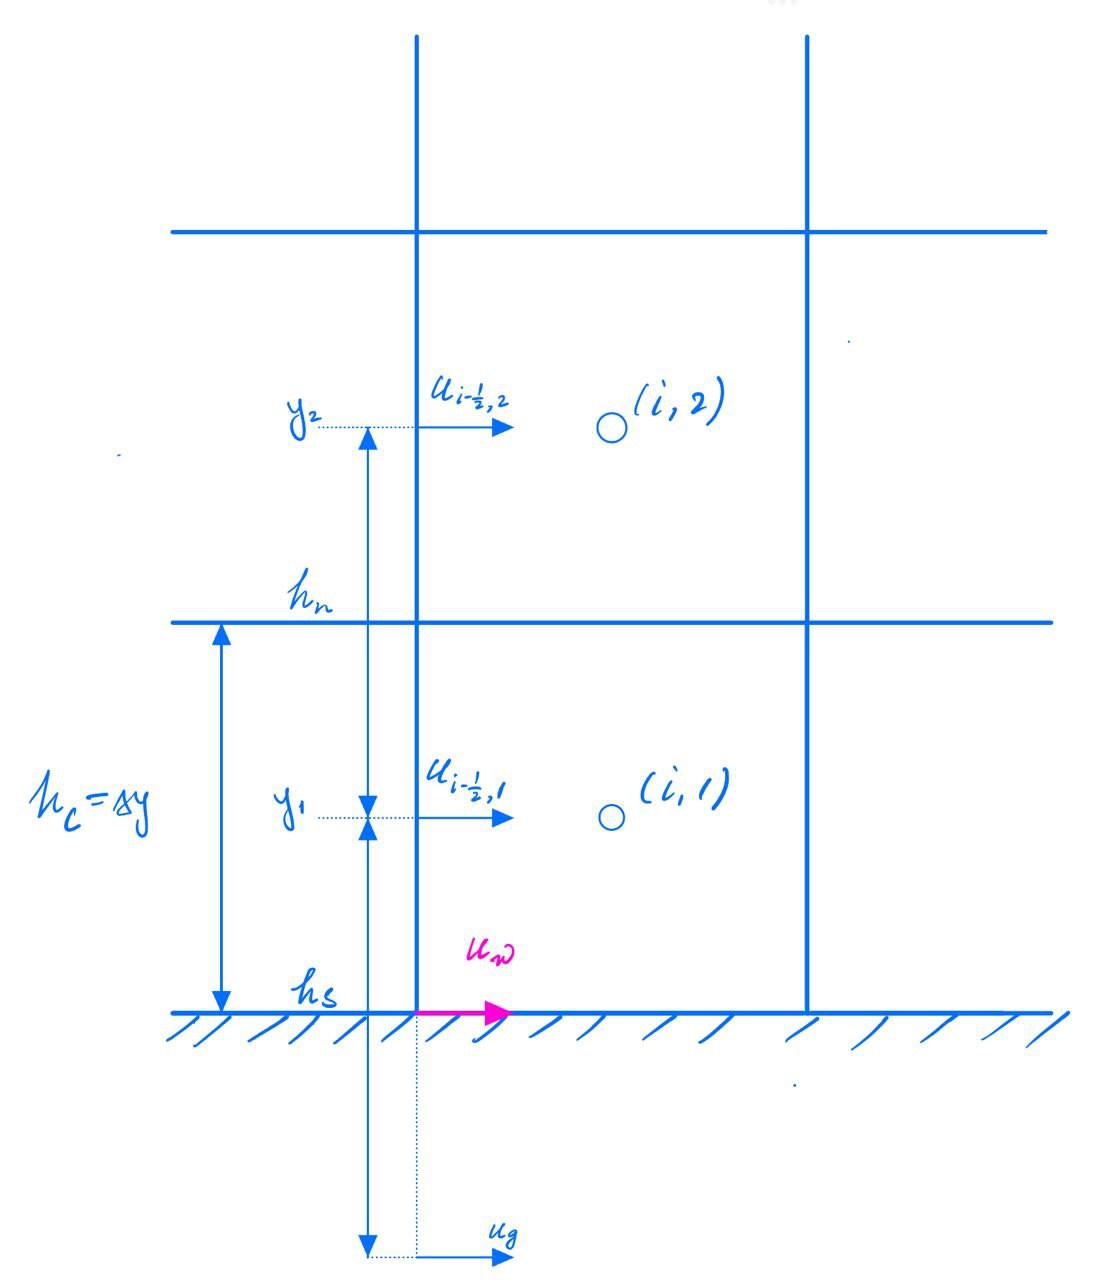
\includegraphics[width=0.45\paperwidth]{Luxx-bottom}
  }
  \caption{$\hat{L}^u_{yy}$ at the bottom boundary.}\label{fig:luxx-bottom}
\end{figure}

The position of $u_g$ is not fixed, we can make the order of the scheme $O(\Delta y^2)$ if $h_s=h_n$. Interpolation of velocity at the wall $u_{w} =\frac{u_{i-\frac{1}{2},1}+u_g}{2}=0 \Rightarrow u_g=-2 u_{i-\frac{1}{2},1}$, then
\begin{equation}\label{eqn:luxx-bot}
\begin{aligned}
\left.\frac{\partial^2 u}{\partial y^2}\right|_{i-\frac{1}{2},1} 
& =u_{i-\frac{1}{2},2}\left(\frac{1}{h_n h_c}\right)+u_{i-\frac{1}{2},1}\left(\frac{-2}{h_n h_s}+\frac{-2}{h_s h_c}\right) \\
& =u_{i-\frac{1}{2},2}\left(\frac{1}{h_n h_c}\right)+u_{i-\frac{1}{2},1}\left(\frac{-2 h_c-2 h_n}{h_s h_c h_n}\right).
\end{aligned}
\end{equation}
The coefficients from \cref{eqn:luxx-bot} are distributed into the $\hat{L}^u_{yy}$ matrix similarly to previous boundary cases.

\subsubsection{Right boundary.}\label{subsubsec:laplacian-right}
\begin{figure}[H] % here, bottom, top
  \centering{
  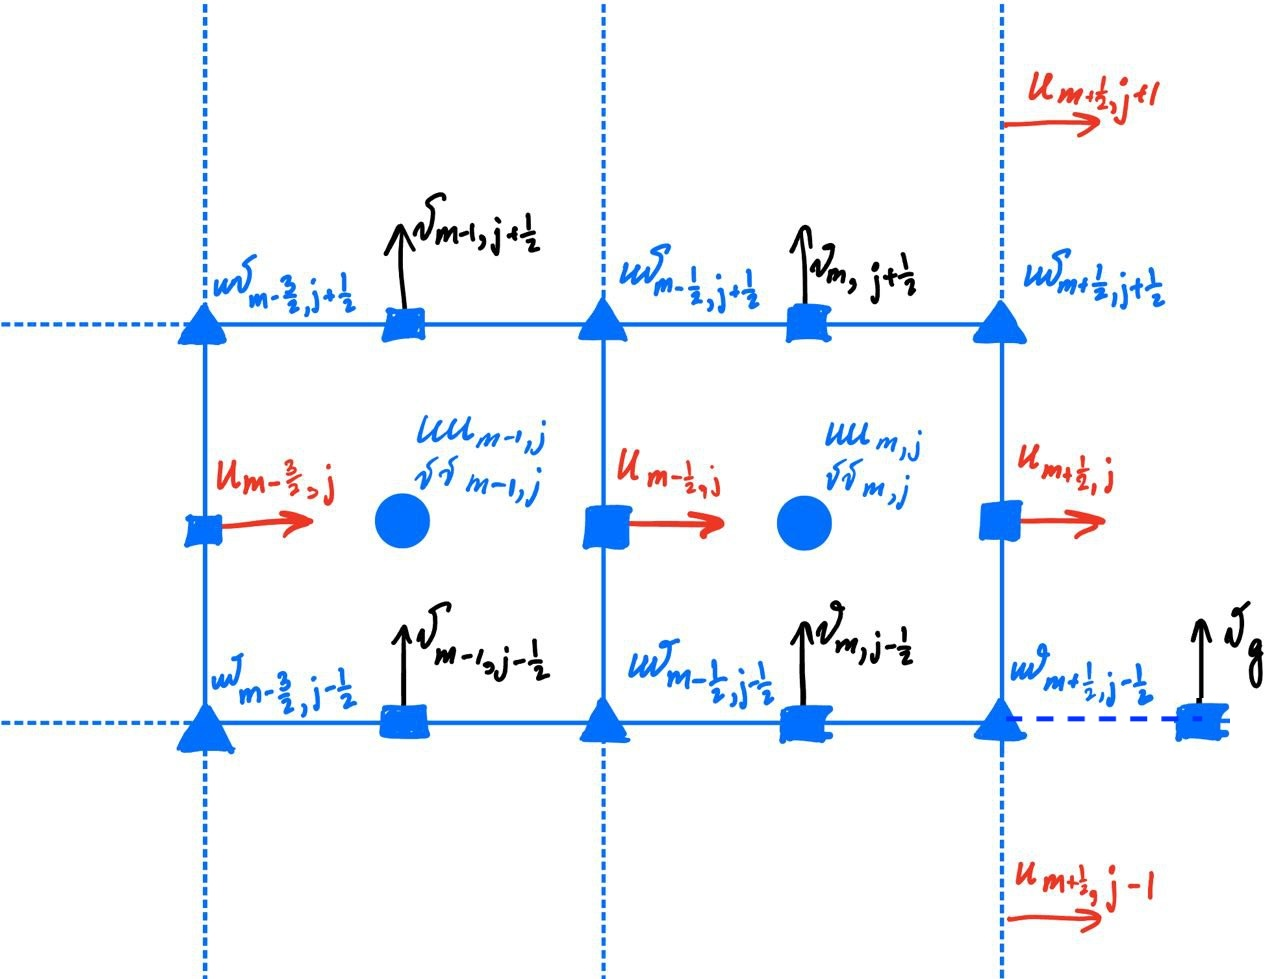
\includegraphics[width=0.45\paperwidth]{ADV-right}
  }
  \caption{$\hat{L}^u_{xx},\hat{L}^v_{xx}$ at the right boundary ($m=M$).}\label{fig:luxx-right-first}
\end{figure}
In order to express the rightmost unknown velocity component $u_{M-\frac{1}{2},j}$ inside the domain it is required to use the boundary values of $u_{M+\frac{1}{2},j}$ and ghost elements for $v_g$ as in \cref{fig:luxx-right-first}. The best case scenario would be to have Dirichlet velocity values $\boldsymbol{v}(t,1,y)\subset \mathbb{R}$ or Neumann boundary condition $\left.\frac{\partial u}{\partial x}\right|_{M+\frac{1}{2},j}=0$ as in Colonius-Taira~\cite{Colonius:2008} at the outlet. However, since the solution of \cref{eqs:NSE-dsm-bl} at the right boundary of the domain might not have the same behaviour, it is not possible to impose such boundary conditions for our problem statement. We will address the spatial discretization of Laplacian at the right boundary in \cref{subsec:laplacian-ABC}.

%%%%%%%%%%%%%%%%%%%%%%%%%%%%%%%%%%%%%%%%%%%%%%%%
\subsection{Advection}\label{subsec:advection}

%\begin{figure}
%\centering
%{\includegraphics[width=0.75\paperwidth]{advectionGrid.jpg} }
%\caption{\small Advection on a staggered grid.}\label{fig:advectionGrid}
%\end{figure}
Since Explicit Adams-Bashforth~\cref{eqn:nonlinear-adams-bashforth} uses information from time steps $n$ and $n-1$, while we solve the system of equations for time step $n+1$ there is no need for upwinding or even more complicated schemes. For spatial discretization we will try to stick to the central schemes as they are more stable and less dependent on the flow direction. It is convenient to write such schemes for conservative form of the advection, moreover, this also keeps the error low, since there is no product of velocity with acceleration. Hence, let us rewrite advective derivatives in conservative form. 
\begin{align}\label{eqn:advection-conservative}
	u\frac{\partial u}{\partial x}+v \frac{\partial u}{\partial y}
	&=u\frac{\partial u}{\partial x}+0+v \frac{\partial u}{\partial y}\nonumber\\
	&= u\frac{\partial u}{\partial x}+ u\left(\frac{\partial u}{\partial x} +\frac{\partial v}{\partial y}\right ) +v \frac{\partial u}{\partial y}\nonumber\\
	&=\left(u\frac{\partial u}{\partial x}+ u\frac{\partial u}{\partial x}\right ) +\left(u\frac{\partial v}{\partial y} +v \frac{\partial u}{\partial y}\right )\nonumber\\
	&=\frac{\partial uu}{\partial x}+ \frac{\partial uv}{\partial y}.
\end{align}
Our goal is to compute advection components at the unknown velocity coordinates. Below we will describe the discretization schemes for \cref{eqn:advection-conservative}. 

\subsubsection{Inner part}\label{subsubsec:advection-inner}
Advective component from $x$-momentum was expressed in conservative form by \cref{eqn:advection-conservative}. It is discretized using the standard central differencing schemes~\cite{Colonius:2008} as
\begin{align}\label{eqn:adv-inner}
	\left (u\frac{\partial u}{\partial x}+v \frac{\partial u}{\partial y}\right)_{i-\frac{1}{2},j}&=\frac{(uu)_{i
	,j}-(uu)_{i- 1,j}}{\frac{\Delta x_i+\Delta x_{i-1}}{2}}+\frac{(uv)_{i-\frac{1}{2},j+\frac{1}{2}}-(uv)_{i-\frac{1}{2},j-\frac{1}{2}}}{\Delta y_i},
\end{align}
which is evaluated at the same points as $u_{i-\frac{1}{2},j}$ (squares in \cref{fig:ADV}). We need to compute $uv$ at the nodes and $uu$ at cell centres, which are triangles and circles respectively in \cref{fig:ADV}. Using linear interpolation~\cite{Colonius:2008} of velocity values leads to
\begin{align*}
  (uu)_{i,j}&=\left(\frac{u_{i+\frac{1}{2},j}+u_{i-\frac{1}{2},j}}{2}\right)^2,\\
  (uv)_{i-\frac{1}{2},j-\frac{1}{2}}&=\left(u_{i-\frac{1}{2},j-1} + \frac{\Delta y_{j-1}}{2}\frac{u_{i-\frac{1}{2},j}-u_{i-\frac{1}{2},j-1}}{\frac{\Delta y_{j-1} +\Delta y_j}{2}} \right) \left( v_{i-1,j-\frac{1}{2}} + \frac{\Delta x_{i-1}}{2}\frac{v_{i,j-\frac{1}{2}}-v_{i-1,j-\frac{1}{2}}}{\frac{\Delta x_{i-1} +\Delta x_i}{2}}\right)\\
  &=\left(\frac{u_{i-\frac{1}{2},j}\Delta y_{j-1} +u_{i-\frac{1}{2},j-1}\Delta y_j}{\Delta y_{j-1}+\Delta y_{j}}\right )\left ( \frac{v_{i,j-1\frac{1}{2}}\Delta x_{i-1} +v_{i-1,j-\frac{1}{2}}\Delta x_i}{\Delta x_{i-1}+\Delta x_{i}}\right).
\end{align*}

\begin{figure}[H] % here, bottom, top
  \centering{
  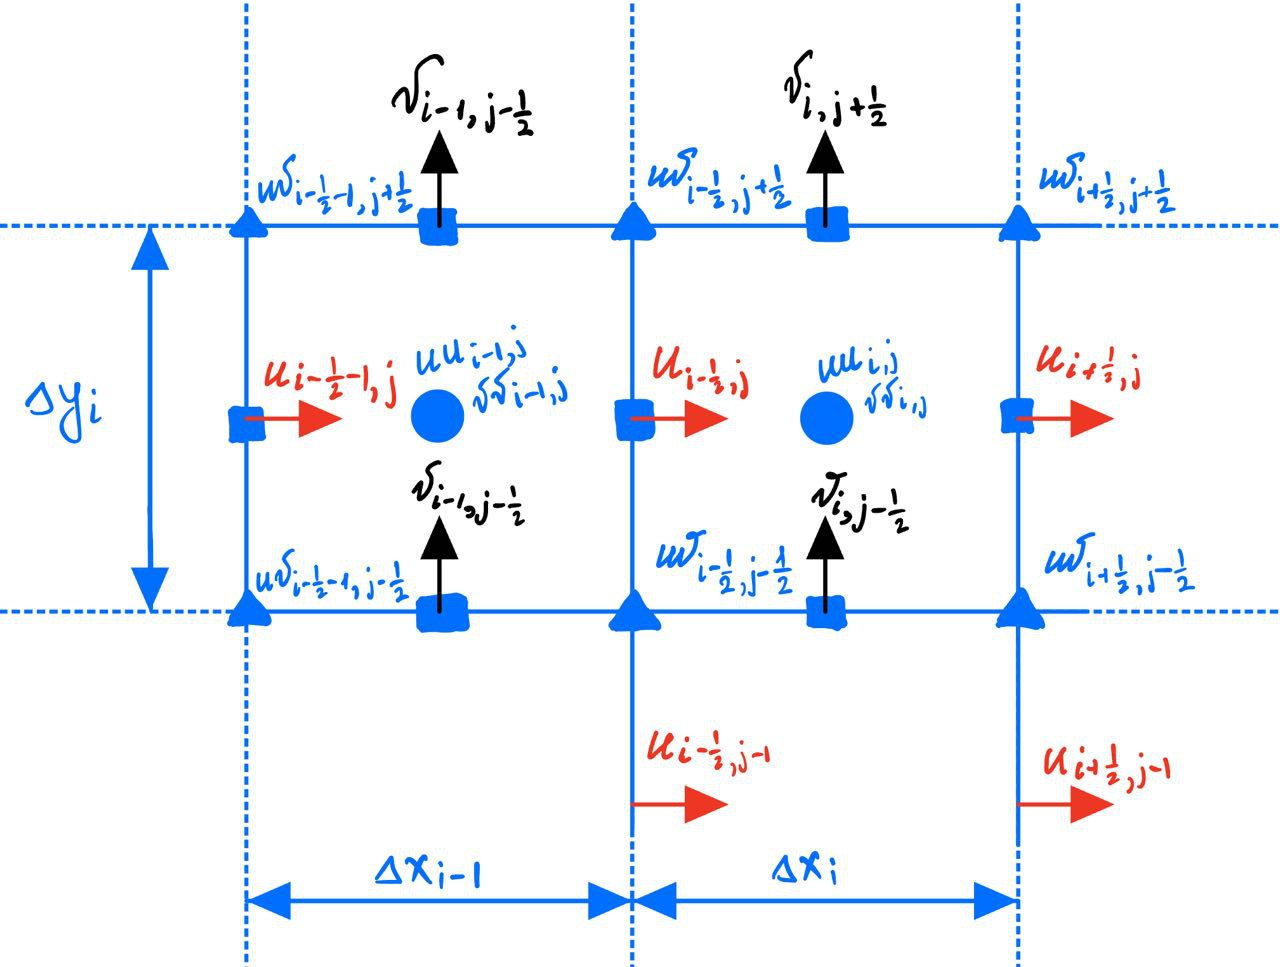
\includegraphics[width=0.65\paperwidth]{ADV}
  }
  \caption{Advection discretization.}\label{fig:ADV}
\end{figure}




%One of the advantages of advective boundary condition $\frac{\partial u}{\partial t}+u\frac{\partial u}{\partial x}=0$ (or  $\frac{\partial u}{\partial t}+u\frac{\partial u}{\partial x}=\epsilon \frac{\partial^2 u}{\partial y^2}$) is that it can be used to express $\frac{\partial uu}{\partial x}$ in terms of transient term as 
%\begin{equation}
%	\left( \frac{\partial uu}{\partial x}\right)_{m+\frac{1}{2},j}=2\left( u \frac{\partial u}{\partial x}\right)_{m+\frac{1}{2},j}=2\left( -\frac{\partial u}{\partial t}\right)_{m+\frac{1}{2},j},
%\end{equation}
%or in terms of transient and diffusive components
%\begin{equation}
%	\left( \frac{\partial uu}{\partial x}\right)_{m+\frac{1}{2},j}=2\left( u \frac{\partial u}{\partial x}\right)_{m+\frac{1}{2},j}=2\left( -\frac{\partial u}{\partial t}+\epsilon\frac{\partial ^2 u}{\partial y^2}\right)_{m+\frac{1}{2},j}.
%\end{equation}
%
%The other advection summand
%\begin{equation}
%	\left(\frac{\partial uv}{\partial y}\right)_{m+\frac{1}{2},j}=\frac{\left( uv \right)_{m+\frac{1}{2},j+\frac{1}{2}}-\left( uv\right)_{m+\frac{1}{2},j-\frac{1}{2}}}{\Delta}
%\end{equation}
%requires values of $v$ at the nodes $m+\frac{1}{2},j\pm \frac{1}{2}$. We may use two neighbouring $v$ components and extrapolate them linearly as 
%\begin{equation}
%	v_{m+\frac{1}{2},j+\frac{1}{2}}=v_{m-1,j\pm\frac{1}{2}}+2\frac{v_{m,j\pm\frac{1}{2}}-v_{m-1,j\pm\frac{1}{2}}}{\Delta x_{m-1}+\Delta x_m}\left(\Delta x_m + \frac{1}{2}\Delta x_{m-1}\right).
%\end{equation}

\subsubsection{Left boundary}\label{subsubsec:advection-left}
\begin{figure}[H] % here, bottom, top
  \centering{
  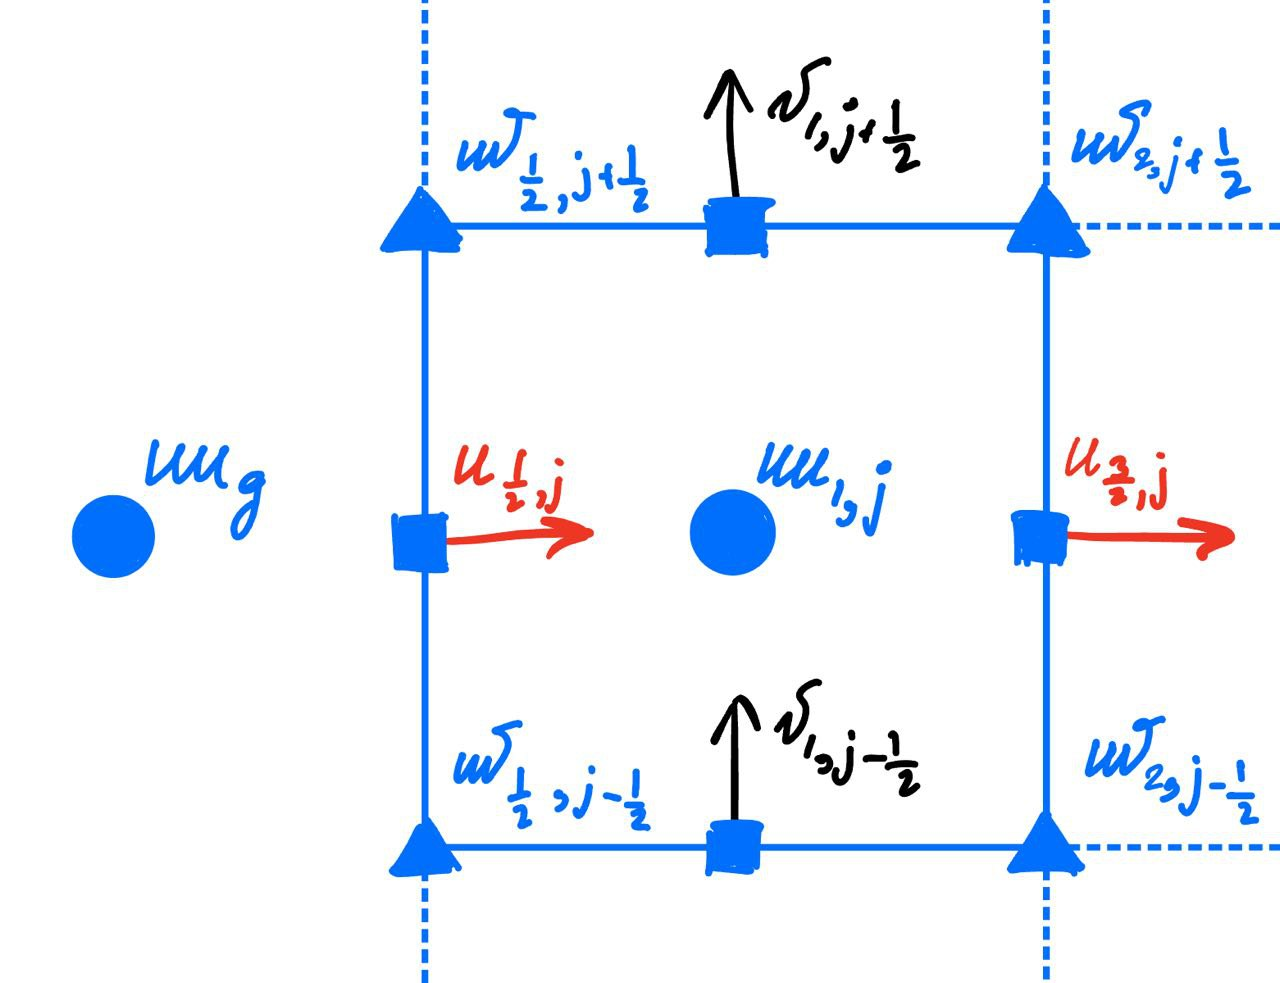
\includegraphics[width=0.30\paperwidth]{ADV-left}
  }
  \caption{Left boundary advection.}\label{fig:ADV-left}
\end{figure}
The exact value of the $uu_g$ element located outside the boundary (\cref{fig:ADV-left}) is known from the inlet boundary conditions, whereas $uv_{\frac{1}{2},j}$ is zero for all $j$ due to $v_{bc}=0$ at the inlet. 

\subsubsection{Top boundary}\label{subsubsec:laplacian-top}
\begin{figure}[H] % here, bottom, top
  \centering{
  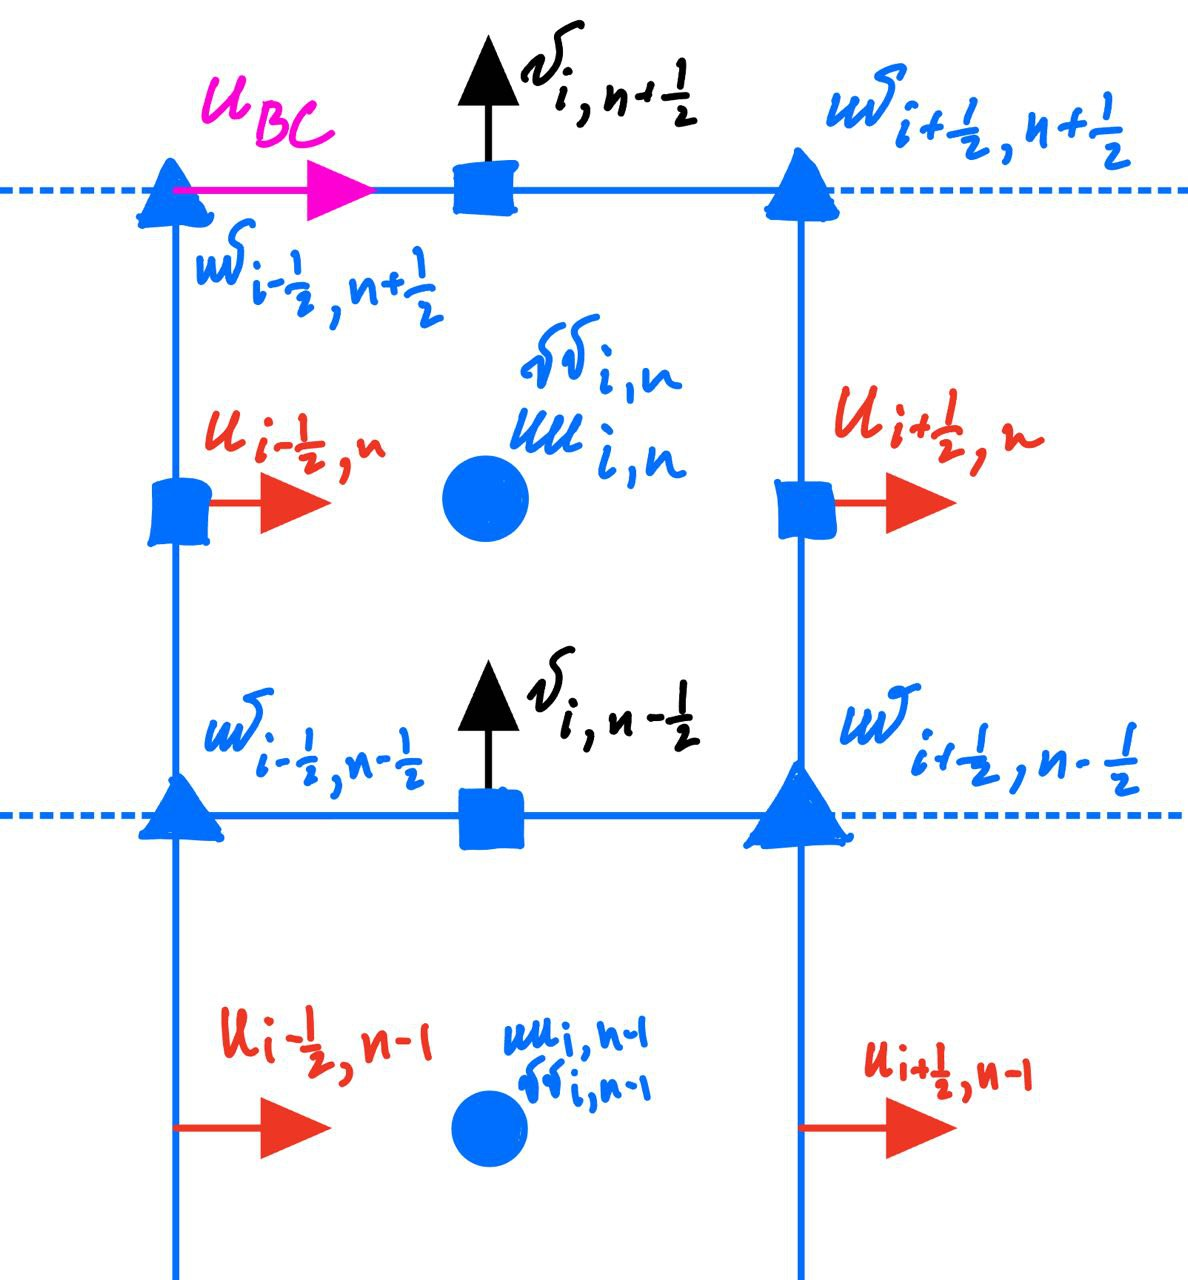
\includegraphics[width=0.35\paperwidth]{ADV-top}
  }
  \caption{Top boundary advection.}\label{fig:ADV-top}
\end{figure}
%The symmetric \cref{eqn:symmetric-bc} defines a mirror surface, which has the same effect on the solution as the semi-infinite boundary condition if the boundary layer thickness is less than the truncated domain height. Mathematically such boundary condition can be written as $v=\frac{\partial v}{\partial y}=0,\frac{\partial p}{\partial y}=0$. 
Since the exact values of the velocity $u_{BC}$ and $v_{BC}=0$ in a freestream are known from \cref{eqn:symmetric-bc}, we can directly use them in our advection term computation making the second summand $uv=0$, in particular
\begin{equation}
	\left( \frac{\partial uu}{\partial x}+\frac{\partial uv}{\partial y}\right)_{i-\frac{1}{2},N}=2\frac{\left( uu\right)_{i,N}-\left( uu\right)_{i-1,N}}{\Delta x_i + \Delta x_{i-1}}+0.
\end{equation}

\subsubsection{Bottom boundary}\label{subsubsec:advection-bottom}
\begin{figure}[H] % here, bottom, top
  \centering{
  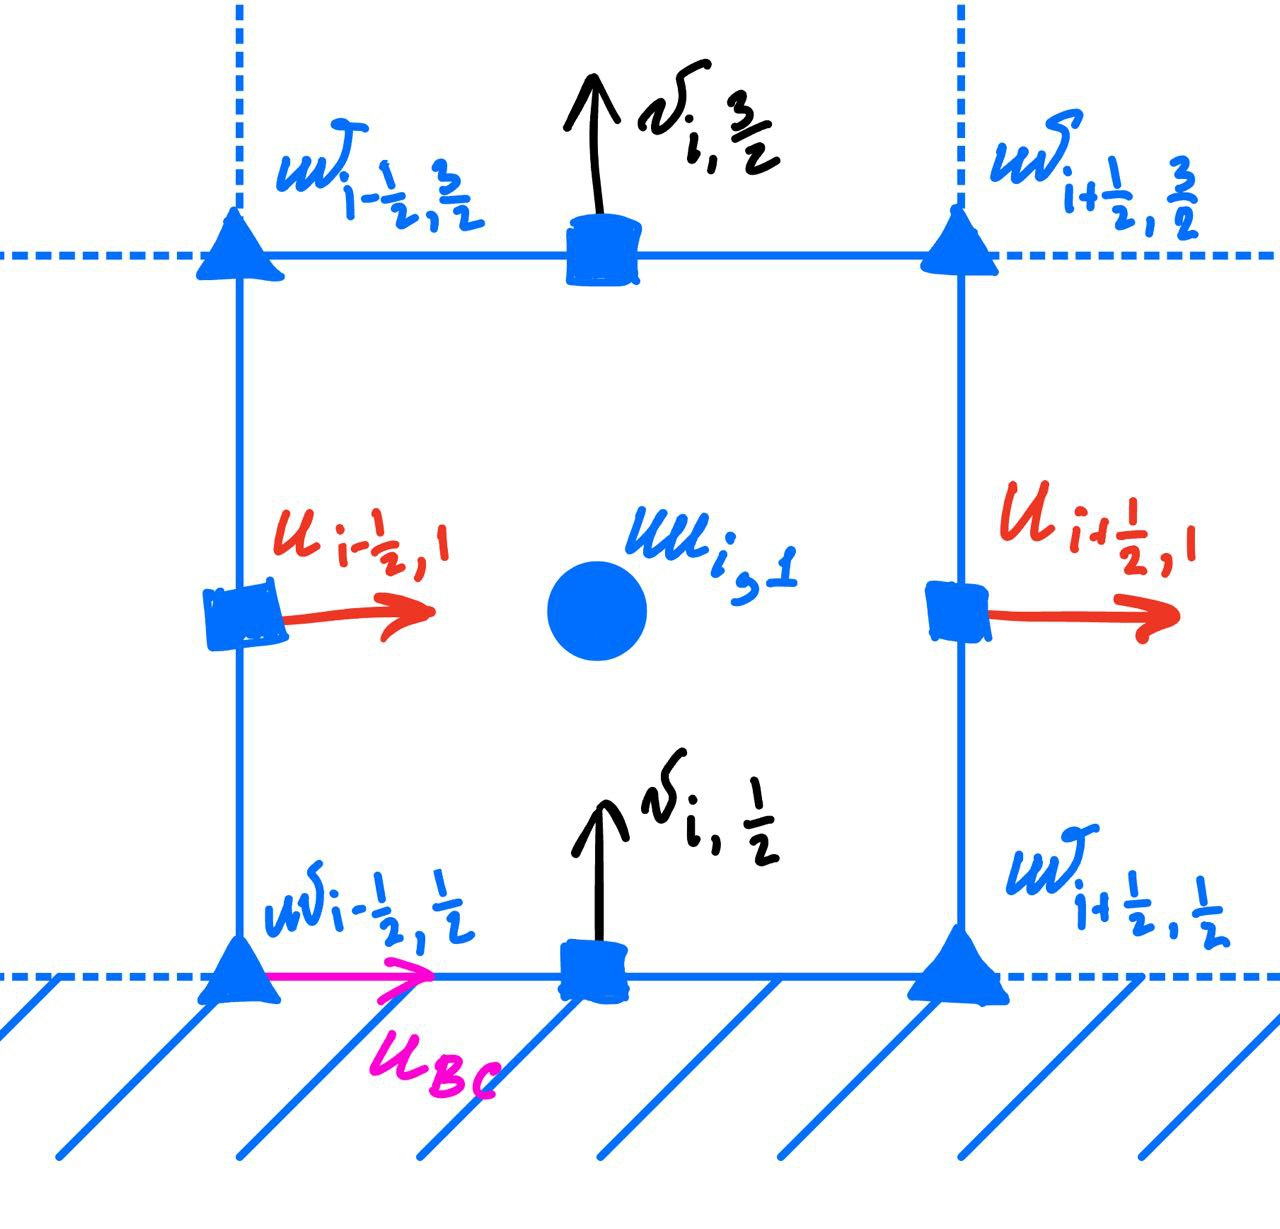
\includegraphics[width=0.30\paperwidth]{ADV-bottom}
  }
  \caption{Bottom boundary advection}\label{fig:ADV-bottom}
\end{figure}
Computation of the advective terms just above the bottom boundary is the same as for the inner part, with the only exception being $uv_{i-\frac{1}{2},\frac{1}{2}}=0$ at the boundary, due to the $u_{bc}=0$ condition on the plate (purple on \cref{fig:ADV-bottom}).

The advective terms in the $y$-momentum equation are computed similarly. After the derivatives are evaluated, they are moved to the right-hand side as in \cref{eqn:NSE-dsm-bl-system-schemes} and treated explicitly. 

\subsubsection{Right boundary}\label{subsubsec:advection-right}

Similarly to Laplacian for the right side in \cref{subsubsec:laplacian-right} we need explicit values of $u$ and  $v$ at and beyond the boundary. These values are yet to be known, hence, it is not possible to utilize the inner part advection formulas from \cref{subsubsec:advection-inner} to rightmost unknown velocities at time steps $n,n-1$ directly. These values are to be determined using artificial boundary conditions in \cref{subsec:advection-ABC}. 
%%%%%%%%%%%%%%%%%%%%%%%%%%%%%%%%%%%%%%%%%%%%%%
\subsection{Divergence}\label{subsec:divergence}

One of the advantages of the staggered grid is that the discrete divergence $D$ and gradient $G$ operators are equal to the negative transpose of each other. 
%Our goal is to eliminate the pressure from the system, \cref{sec:nullspace-method} will explain the use of this property in detail. 
In this section we will show one side of why this identity is true, the other part could be found in \cref{subsec:gradient}.
The second line of \cref{eqn:nse-matrix} reads
\begin{equation*}
\begin{gathered}
\hat{D}\boldsymbol{v}=\hat{bc}_2,\\
\left[ 
\begin{array}{ll}
\hat{D}_x & \hat{D}_y 	
\end{array}
\right]\left[\begin{array}{l}
u\\
v
\end{array}
\right]=\hat{bc}_2
, \\
\frac{1}{\Delta x} D_x u+\frac{1}{\Delta y} D_y v=\hat{bc}_2, \\
\frac{1}{\Delta _{xy}}\left[\begin{array}{ll}
D_x & D_y
\end{array}\right]\left[\begin{array}{l}
u \Delta y \\
v \Delta x
\end{array}\right]=\frac{1}{\Delta _{xy}} D q=\hat{bc}_2,
\end{gathered}
\end{equation*}
where vector $q$ is referred to as velocity flux, and the matrix $D=[D_x D_y]$ without hat is the divergence matrix of integer coefficients. Matrix
\begin{equation}\label{eqn:delta-xy}
	\Delta _{xy}=
	\begin{bmatrix}{}
		\frac{1}{\Delta x_1\Delta y_1}		&0	&\dots	&0\\
		0		&\frac{1}{\Delta x_2\Delta y_1}	&\dots	&0\\
		\vdots		&\vdots	&\ddots	&\vdots\\
		0		&0	&\dots	&\frac{1}{\Delta x_M\Delta y_N}
	\end{bmatrix}
\end{equation}
is $MN\times MN$ diagonal matrix with entries corresponding to the inverse volumes of cells. 

The second-order central difference scheme was employed in the construction of $D$, the order is consistent with the other spatial schemes. Consider a finite volume $V_{i,j}$, continuity equation for the cell centre is then expressed as
\begin{equation*}
	\left(\frac{\partial u}{\partial x} + \frac{\partial v}{\partial y}\right)_{i,j}=0,
\end{equation*}
which can be discretized at cell centre $i,j$ using central difference schemes into
\begin{equation*}
  \frac{u_{i+\frac{1}{2},j} - u_{i-\frac{1}{2},j}}{\Delta x_i}+  \frac{v_{i,j+\frac{1}{2}} - v_{i,j-\frac{1}{2}}}{\Delta y_j}=0.
\end{equation*}

\begin{figure}[H] % here, bottom, top
  \centering{
  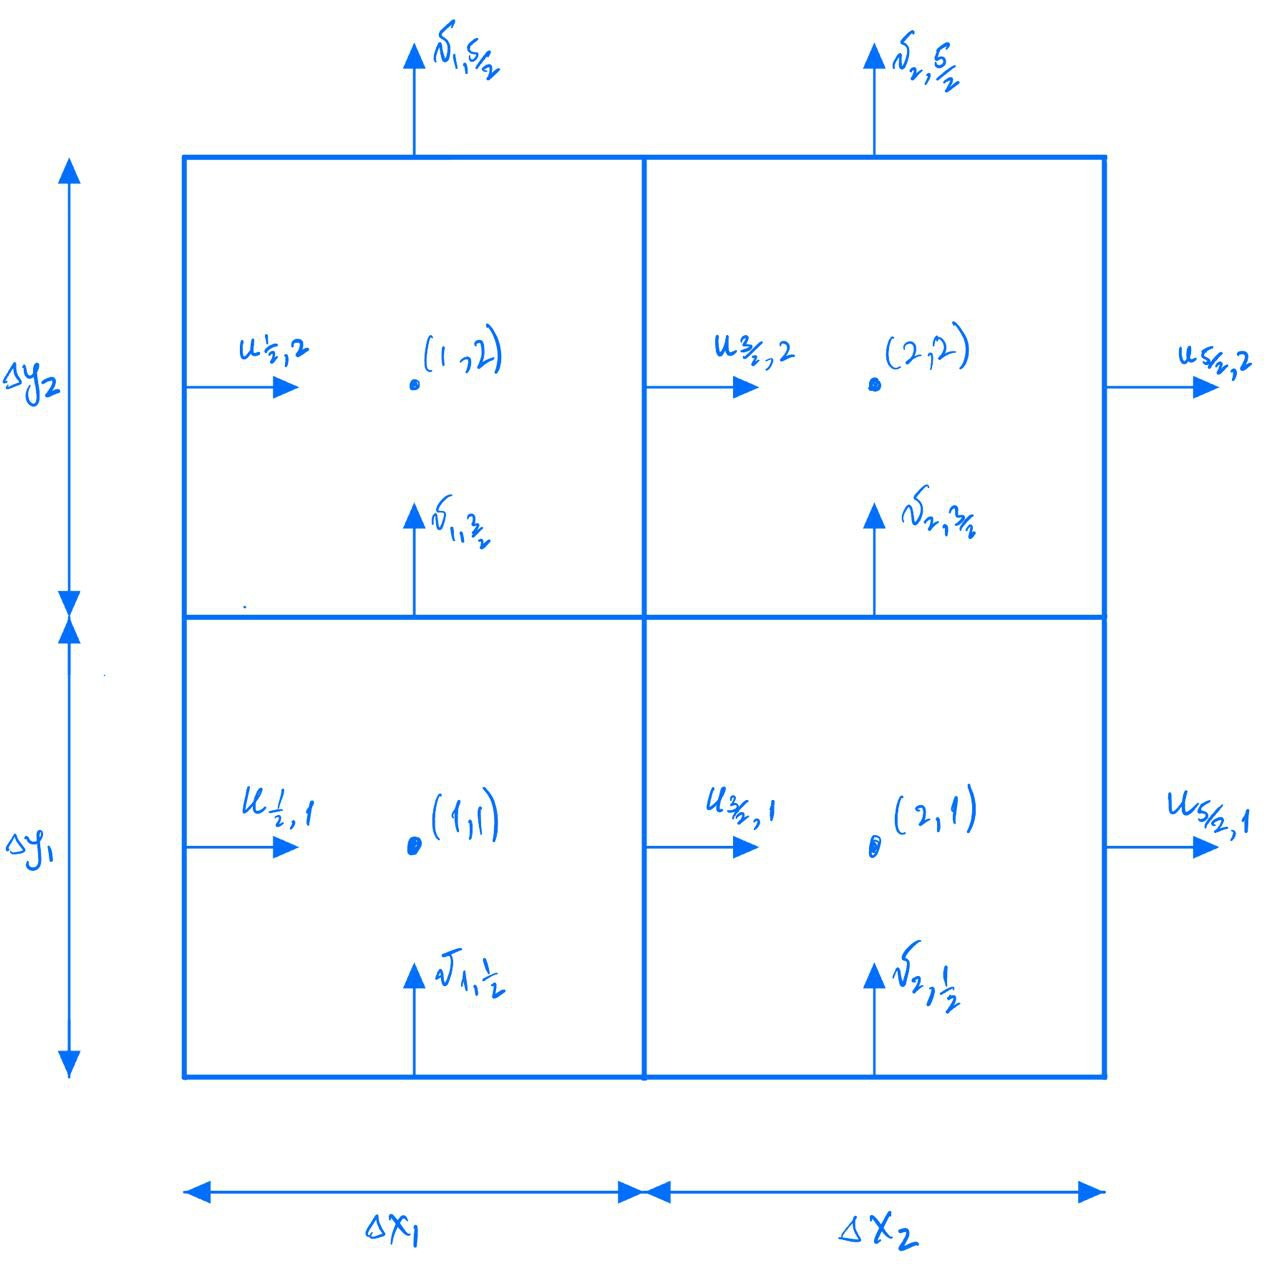
\includegraphics[width=0.45\paperwidth]{D-example-2x2}
  }
  \caption{$2\times 2$ grid example for divergence operator.}\label{fig:D-example-2x2}
\end{figure}

To provide a good visual example, consider $2 \times 2$ grid as in \cref{fig:D-example-2x2} with the same boundary conditions as in \cref{eqs:NSE-dsm-bl}. The partial derivatives of divergence operator evaluated at cell centres are: 
%\begin{equation}
%  \frac{1}{\Delta x_i \Delta y_i}\left[1\quad -1\quad1\quad-1\right] \left[\Delta y_i u_{i+1,j}, \Delta y_i  u_{i,j}, \Delta x_i v_{i,j+1}, \Delta x_i v_{i,j}\right]^T=0.
%\end{equation}
\begin{alignat*}{2}
	V_{1,1}:\frac{u_{\frac{3}{2},1} - u_{\frac{1}{2},1}}{\Delta x_1}+\frac{v_{1,\frac{3}{2}} - v_{1,\frac{1}{2}}}{\Delta y_1}=0,\\
	V_{2,1}: \frac{u_{\frac{5}{2},1} - u_{\frac{3}{2},1}}{\Delta x_2}+\frac{v_{2,\frac{3}{2}} - v_{2,\frac{1}{2}}}{\Delta y_1}=0,\\
	V_{1,2}:\frac{u_{\frac{3}{2},2} - u_{\frac{1}{2},2}}{\Delta x_1}+\frac{v_{1,\frac{5}{2}} - v_{1,\frac{3}{2}}}{\Delta y_2}=0,\\
	V_{2,2}:\frac{u_{\frac{5}{2},2} - u_{\frac{3}{2},2}}{\Delta x_2}+\frac{v_{2,\frac{5}{2}} - v_{2,\frac{3}{2}}}{\Delta y_2}=0.
\end{alignat*}

%\begin{enumerate}
%	\item[$V_{1,1}$]: $\frac{u_{1,2} - u_{1,1}}{\Delta x_1}+\frac{v_{2,1} - v_{1,1}}{\Delta y_1}=0$.
%	\item[$V_{1,2}$]: $\frac{u_{1,3} - u_{1,2}}{\Delta x_2}+\frac{v_{2,2} - v_{1,2}}{\Delta y_1}=0$.
%	\item[$V_{2,1}$]: $\frac{u_{2,2} - u_{2,1}}{\Delta x_1}+\frac{v_{3,1} - v_{2,1}}{\Delta y_2}=0$.
%	\item[$V_{2,2}$]: $\frac{u_{2,3} - u_{2,2}}{\Delta x_2}+\frac{v_{3,2} - v_{2,2}}{\Delta y_2}=0$.
%\end{enumerate}

After applying the boundary conditions to the above equations, we obtain the system
\begin{equation}\label[system]{eqn:divergence-matrix}
	\begin{bmatrix}{}
		\frac{1}{\Delta x_1\Delta y_1}		&0	&0	&0\\
		0		&\frac{1}{\Delta x_2\Delta y_1}	&0	&0\\
		0		&0	&\frac{1}{\Delta x_1\Delta y_2}	&0\\
		0		&0	&0	&\frac{1}{\Delta x_2\Delta y_2}
	\end{bmatrix}
	\begin{bmatrix*}[r]{}
		1	&0	&1	&0\\
		-1	&0	&0	&1\\
		0	&1	&-1	&0\\
		0	&-1	&0	&-1
	\end{bmatrix*}
	\begin{bmatrix}{}
	u_{\frac{3}{2},1}	\Delta y_1\\
	u_{\frac{3}{2},2}	\Delta y_2\\
	v_{1,\frac{3}{2}}	\Delta x_1\\
	v_{2,\frac{3}{2}}	\Delta x_2\\
	\end{bmatrix}
	=
	\begin{bmatrix}{}
	\frac{u_{\frac{1}{2},1}}{\Delta x_1}		+	\frac{v_{1,\frac{1}{2}}}{\Delta y_1}\\
	-\frac{u_{\frac{5}{2},1}}{\Delta x_2}	+ 	\frac{v_{2,\frac{1}{2}}}{\Delta y_1}\\
	\frac{u_{\frac{1}{2},2}}{\Delta x_1} 	-	\frac{v_{1,\frac{5}{2}}}{\Delta y_2}\\
	-\frac{u_{\frac{5}{2},2}}{\Delta x_2}		-\frac{v_{2,\frac{5}{2}}}{\Delta y_2}	
	\end{bmatrix},
\end{equation}
which in general case is written as 
$\frac{1}{\Delta_{xy}} D q=\hat{bc}_2$.
The velocity values known at the boundaries are shifted to the right-hand side and explicitly treated. The divergence matrix $D$ contains $\pm1$, as shown in \cref{eqn:divergence-matrix}.

%\begin{figure}[hbt] % here, bottom, top
%  \centering{
%  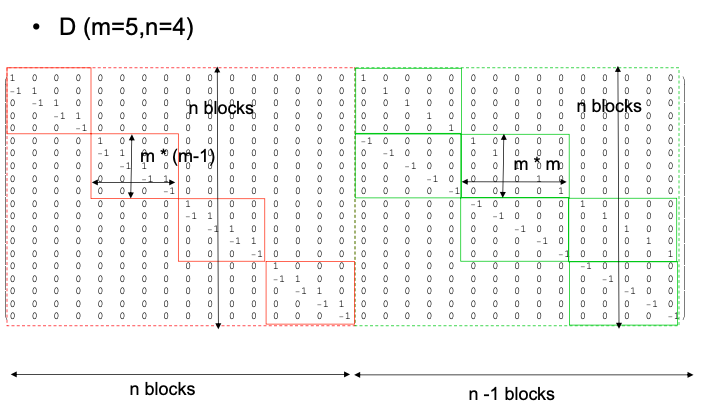
\includegraphics[width=0.75\paperwidth]{D-matrix}
%  }
%  \caption{Divergence matrix.}\label{fig:divergence-matrix}
%\end{figure}

%%%%%%%%%%%%%%%%%%%%%%%%%%%%%%%%%%%%%%%%%%%%%%
% MIGHT WANT TO INCLUDE DERIVATION OF NON-UNIFORM DP/DX 
%% MIGHT ALSO NEED TO CHECK WITH THE PREMULTIPLICATION OF DELTA X
\subsection{Gradient}\label{subsec:gradient} 

The pressure gradients are computed at the same coordinates as the unknown velocities according to \cref{eqn:nse-matrix}. Below we will arrive to the conclusion that the discrete gradient and divergence operators satisfy
\begin{equation}\label{eqn:g-dt}
  {G}=-{D^T}
\end{equation}
on staggered/MAC grids. 

\begin{figure}[H] % here, bottom, top
  \centering{
  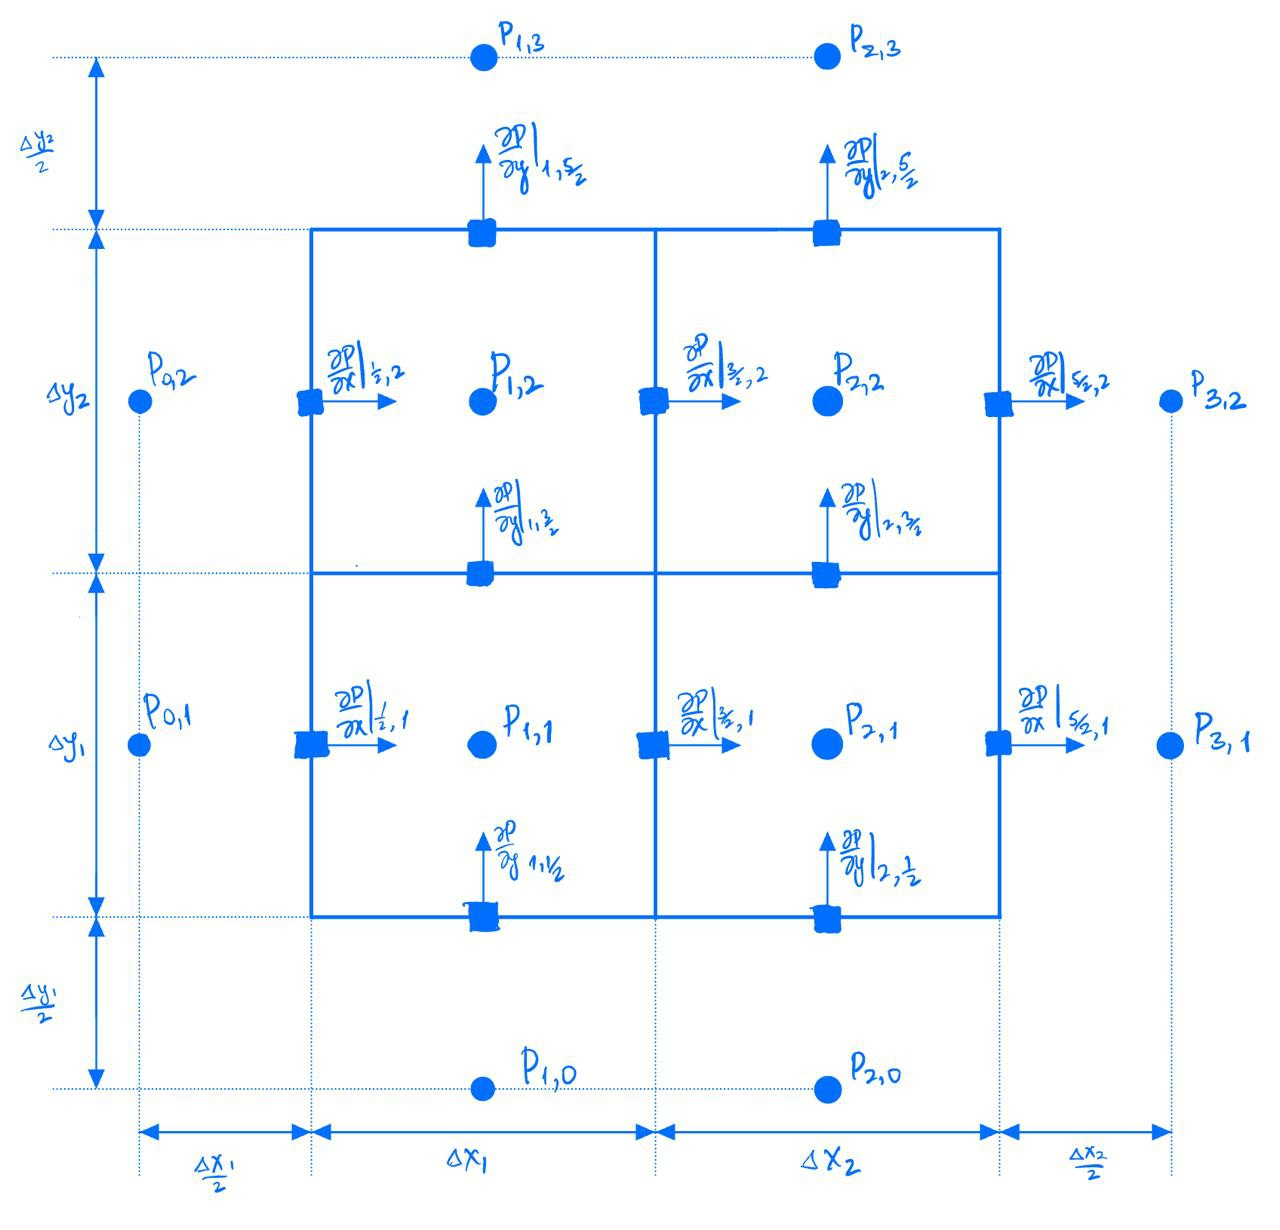
\includegraphics[width=0.65\paperwidth]{G-example-2x2}
  }
  \caption{$2\times 2$ grid example for gradient operator.}\label{fig:G-example-2x2}
\end{figure}


As an illustrative example, we may consider a $2\times 2$ grid as in \cref{fig:G-example-2x2} with the same boundary conditions as in \cref{eqs:NSE-dsm-bl}. It is required to determine the pressure gradients across each unknown velocity (square nodes on \cref{fig:G-example-2x2}):

\begin{alignat*}{2}
	\left.\frac{\partial P}{\partial x}\right|_{\frac{3}{2},1} &=&	\frac{2}{{\Delta x_1 + \Delta x_2}}&\left(P_{1,2}-P_{1,1}\right),\\
	\left.\frac{\partial P}{\partial x}\right|_{\frac{3}{2},2} &=&	\frac{2}{{\Delta x_1 + \Delta x_2}}&\left( P_{2,2}-P_{2,1} \right),\\
	\left.\frac{\partial P}{\partial y}\right|_{1,\frac{3}{2}} &=&	\frac{2}{{\Delta y_1 + \Delta y_2}}&\left(P_{2,1}-P_{1,1} \right),\\
	\left.\frac{\partial P}{\partial y}\right|_{2,\frac{3}{2}} &=&	\frac{2}{{\Delta y_1 + \Delta y_2}}&\left( P_{2,2}-P_{1,2} \right).
\end{alignat*}

The next step is to rewrite the above expressions in matrix form using the pressure boundary conditions outside the grid. The resultant system of linear equations then becomes
\begin{equation}\label[system]{eqn:gradient-matrix}
	\begin{bmatrix}{}
		\frac{2}{\Delta x_1 + \Delta x_2}	&0	&0	&0	\\
		0	&\frac{2}{\Delta x_1 + \Delta x_2}	&0	&0	\\
		0	&0	&\frac{2}{\Delta y_1 + \Delta y_2}	&0	\\
		0	&0	&0	&\frac{2}{\Delta y_1 + \Delta y_2}\\
	\end{bmatrix}
	\begin{bmatrix*}[r]
	-1 & 1 & 0 & 0 \\
	0 & 0 & -1 & 1 \\
	-1 & 0 & 1 & 0 \\
	0 & -1 & 0 & 1
	\end{bmatrix*}
	\begin{bmatrix}{}
  		P_{1,1} \\
	  	P_{2,1} \\
		P_{1,2} \\
		P_{2,2}
	\end{bmatrix}
	=
	\begin{bmatrix}{}
		0\\
		0\\
		0\\
		0
	\end{bmatrix},
\end{equation}
which can be rewritten as
\begin{equation}
	\hat{M}^{-1}{G} 
	\begin{bmatrix}{}
  		p_{1,1} \\
	  	p_{1,2} \\
	  	\vdots \\
	  	p_{MN}
	\end{bmatrix}
=\hat{bc}_p,
\end{equation}
where $\hat{M}^{-1}$ is the diagonal matrix containing the distances between neighbouring pressure coordinates, ${G}$ is the gradient matrix and $[p_1,p_2,...p_{MN}]^T$ is the vector of pressure values at the cell centres. There are no pressure BC values in $\hat{bc}_p$ since no pressure gradient has to be computed across the boundary. It can be observed from \cref{eqn:divergence-matrix,eqn:gradient-matrix} that \cref{eqn:g-dt} holds and the general case is true by construction.



%\subsubsection{Resulting system}



%%%%%%%%%%%%%%%%%%%%%%%%%%%%%%%%%%%%%%%%%%%%%%%%
%%%%%%%%%%%%%%%%%%%%%%%%%%%%%%%%%%%%%%%%%%%%%%%%
%%%%%%
%%%%%%		TYPOS CHECK FROM BELOW  %%%%%%%%%%%%
%%%%%%
%%%%%%%%%%%%%%%%%%%%%%%%%%%%%%%%%%%%%%%%%%%%%%%%
%%%%%%%%%%%%%%%%%%%%%%%%%%%%%%%%%%%%%%%%%%%%%%%%
%Overall, we have $N_x, N_y$ nodes in the $x$ and $y$ direction respectively. 
%There are $N_u=(N_x-1)N_y+N_y$ elements of $u$, where extra $N_y$ is added to account for the unknown outlet boundary velocities. $N_v=N_x(N_y-1)$ represents the number of velocity components within vector $v$. Define $N_{tot}=N_u+N_v$.
%               
%Then the matrices in equation~\eqref{eqn:nse-matrix} have dimensions of:
%\begin{itemize}
%	\item[$\mathbf{I}$] - [$N_{tot}\times N_{tot}$];
%	\item[$\hat{D}$] - [$(N_xN_y)\times(N_{tot})$];
%	\item[$\hat{G}$] - [$(N_{tot})\times(N_xN_y)$];
%	\item[$\mathbf{\hat{H}}$] - [$N_{tot}\times 1$];
%	\item[$\hat{L}$] - [$N_{tot}\times N_{tot}$];
%	\item[bc] - [$N_{tot}\times 1$], which are inhomogeneous terms from the Boundary Conditions vector.
%\end{itemize}        
%
%Attack the system~\eqref{eqn:nse-matrix} with the following (listed in the appendix) schemes:
%\begin{enumerate}
%	\item[\textbf{Viscous}]: Implicit trapezoidal - Crank Nicholson~\eqref{eqn:crank-nicholson} scheme.  
%  \item[\textbf{Nonlinear (advect.)}]: Explicit Adams-Bashforth~\eqref{eqn:adams-bashforth} as in Figure~\ref{fig:Advection-discretization}. 
%	\item[\textbf{Pressure}]: Implicit Euler~\eqref{eqn:implicit-euler}, however the pressure variable is not used in computations. 
%\end{enumerate}
%
%The above discretization schemes result in the following discretized system:
%\begin{equation*}
%	\begin{bmatrix}
%		\frac{1}{\Delta t}\mathbf{I}-\frac{1}{2}\hat{L} & \hat{G} \\
%		\hat{D} & 0
%	\end{bmatrix}
%	\begin{pmatrix}
%		\boldsymbol{v}^{n+1} \\ 
%		p
%	\end{pmatrix}
%	=
%	\begin{pmatrix}
%		\left[\frac{1}{\Delta t}\mathbf{I}-\frac{1}{2}\hat{L}\right]u^n - \left[\frac{3}{2}\hat{N}(\boldsymbol{v}^n) - \frac{1}{2}\hat{N}(\boldsymbol{v}^{n-1})\right]\\
%		0
%	\end{pmatrix}
%	+
%	\begin{pmatrix}
%		\hat{bc}_1\\
%		\hat{bc}_2
%	\end{pmatrix}.
%\end{equation*}
%
%After introduction of new variables $\hat{A}$ and $\hat{r}^n$ the above system can be rewritten as
%\begin{equation}
%	\begin{bmatrix}
%		\hat{A} & \hat{G} \\
%		\hat{D} & 0
%	\end{bmatrix}
%	\begin{pmatrix}
%		\boldsymbol{v}^{n+1} \\ 
%		p
%	\end{pmatrix}
%	=
%	\begin{pmatrix}
%		\hat{r}^n \\
%		0
%	\end{pmatrix}
%	+
%	\begin{pmatrix}
%		\hat{bc}_1\\
%		\hat{bc}_2
%	\end{pmatrix}.
%\end{equation}
%
%
%\begin{figure}
%\begin{center}
%  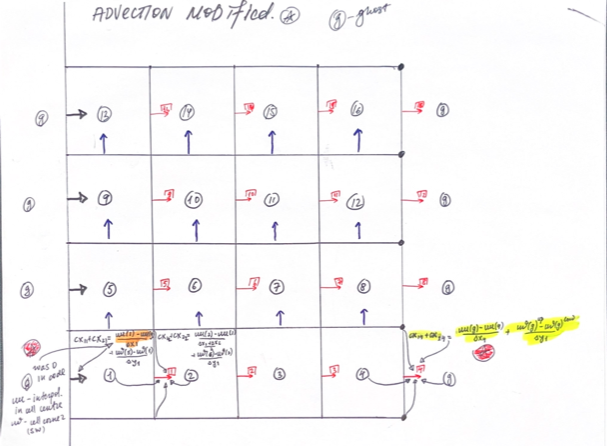
\includegraphics[width=0.75\textwidth]{Figures/advectionGridNew}
%\end{center}
%\caption{Advection discretization.}
%\label{fig:Advection-discretization}
%\end{figure}
%
\section{Artificial boundary conditions}\label{sec:artificial-bc}
Though there are methods that may solve problems on unbounded domains, the majority of the algorithms can only be applied to finite ones. 
%In case of a truncated domain, the introduction of appropriate artificial boundary conditions (ABCs) is crucial for achieving numerical solutions. 
The review papers on such BCs by Sani~\cite{Sani:1994} and Tsynkov~\cite{Tsynkov:1998} list and compare different artificial boundary conditions (ABC) applied to the various flow scenarios. Below we will discuss the options that are most applicable to \cref{eqs:NSE-dsm-bl-dimensional}. 

In solutions of fluid flow, the reflection of waves at the outlet is common. Such behaviour may lead to issues due to incompressibility of the Navier-Stokes equations, i.e. a change of solution near the outlet will affect the solution at the inner part of the domain as well. 
Engquist and Majda\cite{Engquist:1977} introduced one of the earliest and successful tools to address this problem. 
The authors derive a hierarchy of highly absorbing local boundary conditions, serving as approximations to the theoretical nonlocal boundary conditions which were historically used as the only non-reflective options. 
%An essential consideration for practical applications lies in ensuring that these boundary conditions yield well-posed mixed initial boundary value problems. 
Engquist and Majda admit that it is not possible to eliminate all of the reflections, however, it is possible to come up with condition such that for an arbitrary highly singular wave packet only low amplitude smooth reflections occur. %%%%% WHAT DOES THIS MEAN
The main idea of the paper is to transition from space-time domain into frequency domain, factorize the equation at the boundary (within a smooth error) and eliminate the reflected waves.
The methodology outlined was employed by Engquist and Majda to construct absorbing artificial boundaries tailored for the acoustic wave equation in both Cartesian and polar coordinates, as well as for the linearized shallow water equations in two dimensions. 
Although the method is not fully applicable to our problem, the authors systematically addressed and resolved the reflective behaviour of the outlet.

Another way of overcoming the reflective behaviour of the fluid flow was developed by Liu~\cite{Liu:1993}. They studied the spatial instability of planar Poiseuille flow. The governing equations in this paper were solved for perturbed velocity components with tilde $\tilde{u}=u-u_0,\tilde{v}=v-v_0$, where $u_0,v_0$ are mean values of velocity components $u,v$. The general idea is the introduction of an additional buffer domain (\cref{fig:BC-buffer}) at the exit that involves the use of:
\begin{figure}[H] % here, bottom, top
  \centering{
  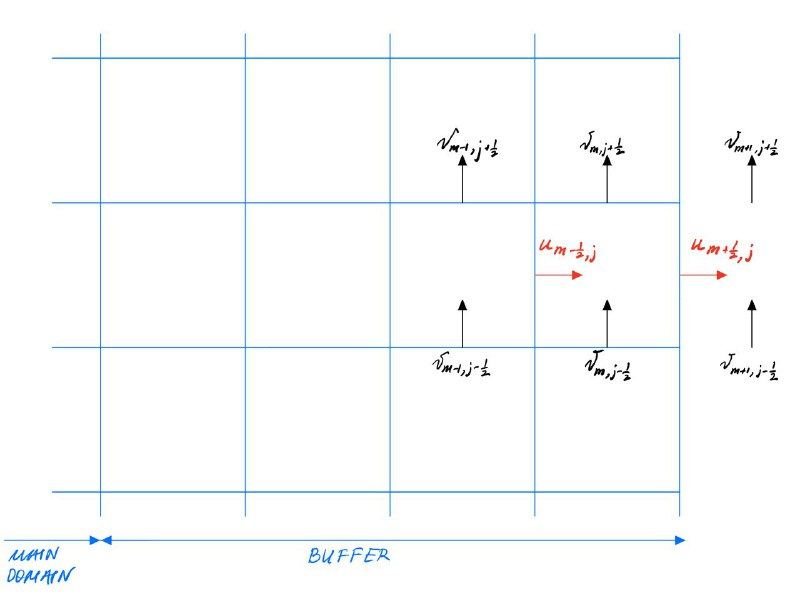
\includegraphics[width=0.45\paperwidth]{BC-Buffer}
  }
  \caption{Buffer BC by Liu.}\label{fig:BC-buffer}
\end{figure}
\begin{enumerate}
	\item Semi-implicit perturbed mass conservation (outlet velocity is updated using the data from inner part at previous time levels)
	\begin{equation*}
		\tilde{u}_{m+\frac{1}{2},j}^{n+1}=\tilde{u}_{m-\frac{1}{2},j}^n-\frac{\tilde{v}^n_{m-1,j+\frac{1}{2}}-\tilde{v}^n_{m-1,j-\frac{1}{2}}}{\Delta y_{j}}{\Delta x_m}.
	\end{equation*}
	\item Linear profile of the tangential velocity component computed semi-implicitly (tangential ghost velocity is updated using the data from inner part at previous time levels) as
	\begin{equation*}
		\frac{\partial ^2 \tilde{v}}{\partial x^2}=0\implies \tilde{v}^{n+1}_{m+1,j-\frac{1}{2}}=2\tilde{v}^n_{m,j-\frac{1}{2}}-\tilde{v}^n_{m-1,j-\frac{1}{2}},
	\end{equation*}
	where $\tilde{v}^{n+1}_{m+1,j-\frac{1}{2}}$ is the ghost component outside the domain.
\end{enumerate}
This buffer was not consistent with the physics and required to be as short as possible. 

Braza and collaborators~\cite{Jin:1993,Kourta:1987,Persillon:1998} considered the shear flow (mixing layer) problem. Authors constructed a set of BCs that allows the eddies to be freely developed downstream as they leave the domain. Furthermore, the most appropriate boundary conditions at the top and bottom were those derived by considering boundaries as streamlines with
\begin{equation}\label[bc]{eqn:symmetric-bc}
	v=0\text{ and } \frac{\partial u}{\partial y}=0,
\end{equation}
while the non-reflective outlet had the following boundary conditions: 
\begin{subequations}
\label[pluralequation]{eqs:braza}
\begin{align}
\label[bc]{eqn:kourta-bc}
	\text{Type I: }&\frac{\partial ^2u}{\partial x^2}=0,\frac{\partial v}{\partial x	}=0,\\
\label[bc]{eqn:Jin-Braza-bc}
	\text{Type II: }&\frac{\partial \boldsymbol{v}}{\partial t}+u\frac{\partial \boldsymbol{v}}{\partial x}-\nu \frac{\partial^2 \boldsymbol{v}}{\partial y^2}=0,
\end{align}
\end{subequations}
where $\nu$ is kinematic viscosity. 
Results shown in \cref{fig:Kourta-Braza-results,fig:Jin-Braza-results} correspond to results obtained through \cref{eqn:kourta-bc,eqn:Jin-Braza-bc}.
	The first \cref{eqn:kourta-bc} made vortices hit against a "wall", while they should have left the domain. 
	However, the second \cref{eqn:Jin-Braza-bc} was derived similarly to Engquist and Majda~\cite{Engquist:1977} and displayed more non-reflective behaviour. 
%	In addition, the numerical algorithm used in the corresponding paper~\cite{Jin:1993} required boundary conditions for auxiliary potential function $\phi$ at the outlet. 
%	The corresponding ABC for $\phi$ was derived from the numerical algorithm by taking into account \cref{eqn:Jin-Braza-bc}. 
%	(It might be possible to obtain an ABC for pressure depending on the algorithm used.)
\begin{figure}[H]
\centering
  \subfigure[Kourta-Braza results.]{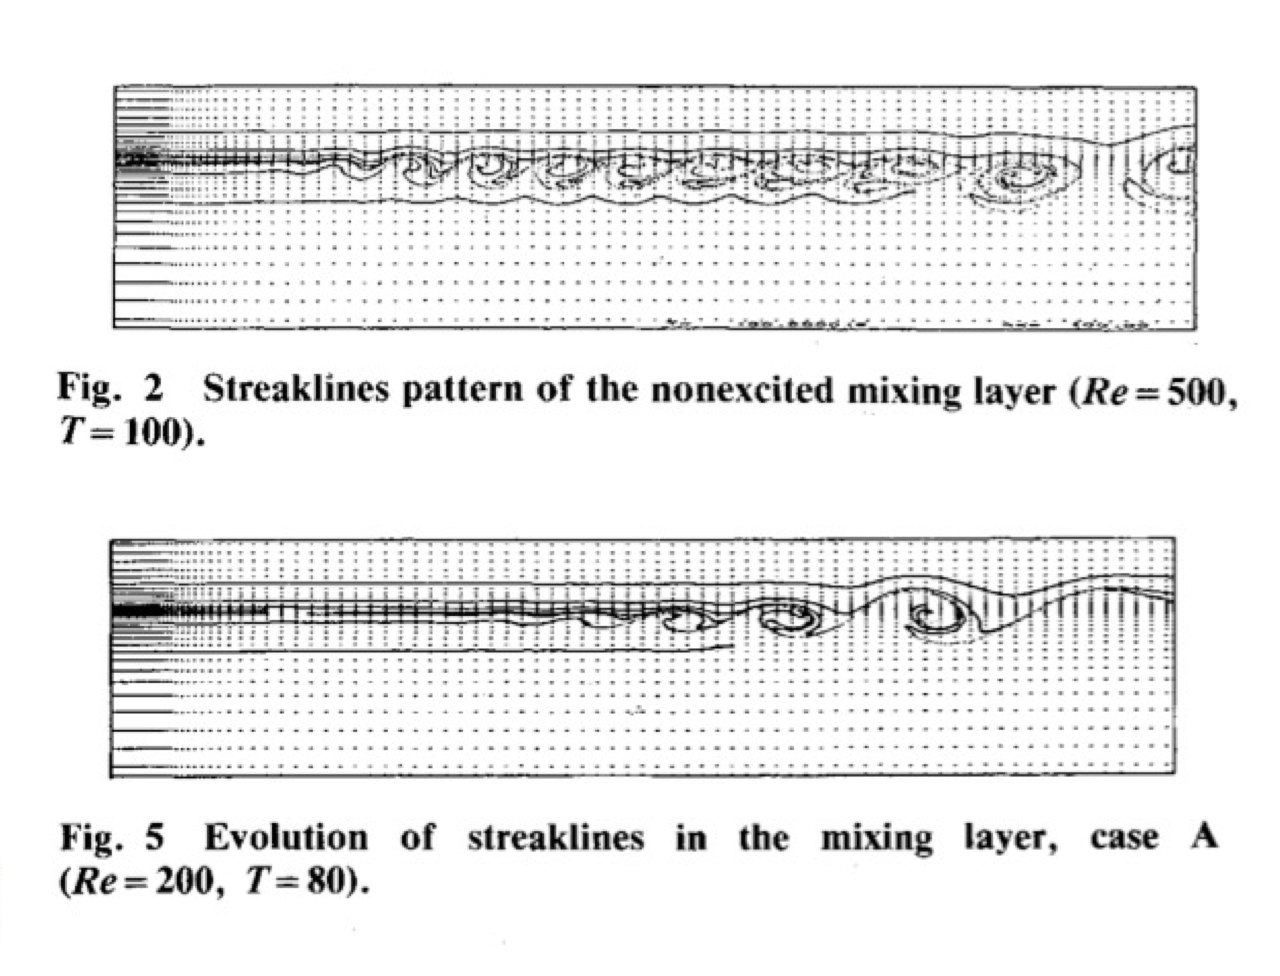
\includegraphics[height=0.265\textwidth]{Kourta-Braza.jpg} \label{fig:Kourta-Braza-results}} \quad
  \subfigure[Jin-Braza-Braza results.]{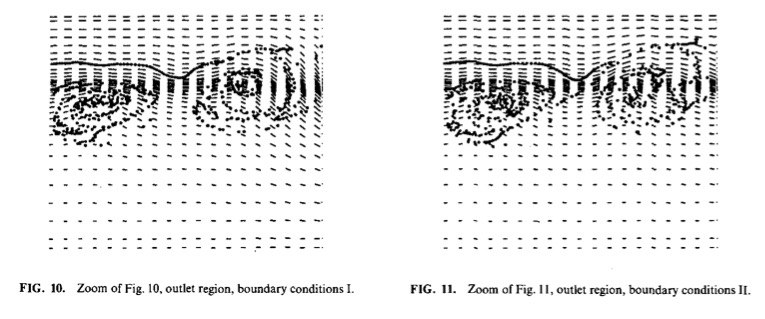
\includegraphics[height=0.245\textwidth]{Jin-Braza.jpg} \label{fig:Jin-Braza-results}}
\caption{\small Resultant streaklines of Braza and collaborators.}
\end{figure}

Taking into account successful results obtained in \cite{Kourta:1987, Jin:1993, Persillon:1998} and similarities between the boundary layer and mixing layer flows we will use
\footnote{G. Fournier and F. Golanski (2008) claim that Prandtl BL solution for advective BCs s.a. $\frac{\partial \boldsymbol{v}}{\partial t} + u\frac{\partial \boldsymbol{v}}{\partial x}=0$ results in wrong solution for pressure gradient, while their condition $\frac{\partial \boldsymbol{v}}{\partial t}+u \frac{\partial \boldsymbol{v}}{\partial x}+v \frac{\partial \boldsymbol{v}}{\partial y}-\nu \frac{\partial^2 \boldsymbol{v}}{\partial y^2}=0$ matches Prandtl BL. Such BC could be used as an alternative option if simple condition from Jin-Braza\cite{Jin:1993} will fail.} 
\cref{eqn:Jin-Braza-bc,eqn:symmetric-bc} as boundary conditions for top and right boundaries respectively and also truncate the domain to width and height $L$.

\subsection{Derivation of Type II ABC (as in paper)}\label{subsec:non-reflecting-abc}
Velocity vector $\boldsymbol{v}$ is considered as the transported wave quantity incident on the boundary. 
Due to the presence of reflective flow behaviour at the outlet, the boundary is said to satisfy the anisotropic wave equation
\begin{equation}\label{eqn:wave-eqn-at-bdry}
	\frac{\partial ^2 \boldsymbol{v}}{\partial t^2}-c_x^2\frac{\partial ^2 \boldsymbol{v}}{\partial x^2}-c_y^2\frac{\partial ^2 \boldsymbol{v}}{\partial y^2}=0,
\end{equation}
where $c_x,c_y$ are the characteristic velocities of $x,y$ wave propagation. The presence of the second time derivative seems to be an "ad-hoc guess" which worked for Jin-Braza\cite{Jin:1993}. 

We can rewrite \cref{eqn:wave-eqn-at-bdry} in terms of pseudo-differential operator
\begin{equation*}
	L\boldsymbol{v}\equiv -D_t^2\boldsymbol{v}+c_x^2D_x^2\boldsymbol{v}+c_y^2D_y^2\boldsymbol{v=0},
\end{equation*}
where $D^2_x,D^2_y$ and $D^2_t$ are second derivatives w.r.t. $x,y$ and $t$ variables respectively. 

Operator $L$ can be factored into
\begin{equation*}
	L\boldsymbol{v}=L^+L^-\boldsymbol{v}=0,
\end{equation*}
where
\begin{align*}
	L^+&\equiv c_x D_x + D_t\sqrt{1-\left( \frac{c_y D_y}{D_t}\right)^2},\\
	L^-&\equiv c_x D_x - D_t\sqrt{1-\left( \frac{c_y D_y}{D_t}\right)^2}\\
\end{align*}
correspond to waves travelling inside and outside the domain in directions parallel to the $x$ axis. 

To nullify the reflected waves, a total absorption~\cite{Engquist:1977} at the boundary
\begin{equation}\label{eqn:absorb-incoming}
	L^+\boldsymbol{v}=0
\end{equation}
is considered. It is possible to use the Taylor series to approximate the square root term, however, the results were found to be strongly ill posed, whereas, Pade second approximation
\begin{equation}\label{eqn:pade-second}
	\sqrt{1-\left( \frac{c_y D_y}{D_t}\right)^2}\approx1-\frac{1}{2}\left( \frac{c_y D_y}{D_t}\right)^2
\end{equation}
turned out to be well posed~\cite{Engquist:1977,Kreiss:1970} . It is possible to rewrite \cref{eqn:absorb-incoming} in terms of \cref{eqn:pade-second} as
\begin{equation*}
	\left( c_xD_x + D_t - \frac{c^2_y}{2D_t}D_y^2 \right)\boldsymbol{v}=0,
\end{equation*}
which can be matched to the momentum Navier-Stokes equation as
\begin{equation}\label[bc]{eqn:absorbing-bc-dimensional}
	\frac{\partial \boldsymbol{v}}{\partial t} + u\frac{\partial \boldsymbol{v}}{\partial x}-\epsilon\frac{\partial ^2 \boldsymbol{v}}{\partial y^2}=0.
\end{equation}
\subsection{Laplacian at the right boundary using ABC}\label{subsec:laplacian-ABC}
%The aim is to make a second order scheme for the first derivative to keep consistency with the discretization of the inner part. Take the right most nodes, the aim is to eliminate the second derivative in equations below, cross multiply by coefficients to make up a common factor at second derivative, then subtract the equations. 
%	\begin{equation}
%	\begin{aligned}
%	& u_m=u_{m+1}+\left.\left(x_m-x_{m+1}\right) \frac{\partial u}{\partial x}\right|_{m+1}+\left.\frac{\left(x_m-x_{m+1}\right)^2}{2 !} \frac{\partial^2}{\partial x^2}\right|_{m+1}+\ldots \bigg/\frac{\left(x_{m-1}-x_{m+1}\right)^2}{2}. \\
%	& u_{m-1}=u_{m+1}+\left.\left(x_{m-1}-x_{m+1}\right) \frac{\partial u}{\partial x}\right|_{m+1}+\left.\frac{\left(x_{m-1}-x_{m+1}\right.}{2 !} \frac{\partial^2}{\partial x^2}\right|_{m+1}+\ldots \bigg/ \frac{\left(x_m-x_{m+1}\right)^2}{2}.
%	\end{aligned}
%	\end{equation}
%
%After subtracting and simplifying the expression for the first partial derivative reduces to
%\begin{equation}
%\frac{\partial u}{\partial x}\bigg|_{m+1}=\frac{-u_{m-1}{\left(x_m-x_{m+1}\right)^2}+u_m{\left(x_{m-1}-x_{m+1}\right)^2}-u_{m+1}{\left(x_{m-1}-x_m\right)\left(\left[x_{m-1}-x_{m+1}\right]+\left[x_m-x_{m+1}\right]\right)}}{{\left(x_m-x_{m+1}\right)\left(x_{m-1}-x_{m+1}\right)\left(x_{m-1}-x_m\right)}}.
%\end{equation}
%
%By applying simple Neumann boundary condition $\frac{\partial u}{\partial x}\big|_{m+1}=0$ we can express the right most value of the velocity with respect to the other two as
%\begin{equation}
%u_{m+1}=\frac{-u_{m-1}\left(x_m-x_{m+1}\right)^2+u_m\left(x_{m-1}-x_{m+1}\right)^2}{\left(x_{m-1}-x_m\right)\left(x_{m-1}-x_{m+1}+x_m-x_{m+1}\right)},
%\end{equation}
%which can be plugged into the boundary value in laplacian discretization \eqref{eqn:laplacian-discretization-non-uniform-dx} to obtain
%
%\begin{equation}
%\begin{aligned}
%\left.\frac{\partial^2 u}{\partial x^2}\right|_m & =\frac{\left[u_{m-1} \frac{-h_e^2}{h_w\left(2 h_e+h_w\right)}+u_m \frac{\left(h_e+h_w\right)^2}{h_w\left(2 h_e+h_w\right)}\right] h_w-u_m ( 2 h_c)+u_{m-1} (h_e)}{h_e h_w h_c}, \\
%& =u_{m-1}\left[\frac{1}{h_w h_c}-\frac{h_e}{h_w h_d\left(2 h_e+h_w\right)}\right]+u_m\left[\frac{2 \frac{h_e+h_w}{2}}{h_e h_w h_c}+\frac{\left(h_e+h_w\right)^2}{h_e h_w h_c\left(2 h_e+h_w\right)}\right].
%\end{aligned}
%\end{equation}
%\textbf{ To be determined.}\textbf{ To be determined.}\textbf{ To be determined.}\textbf{ To be determined.}\textbf{ To be determined.}\textbf{ To be determined.}\textbf{ To be determined.}\textbf{ To be determined.}\textbf{ To be determined.}\textbf{ To be determined.}\textbf{ To be determined.}\textbf{ To be determined.}\textbf{ To be determined.}\textbf{ To be determined.}\textbf{ To be determined.}\textbf{ To be determined.}\textbf{ To be determined.}\textbf{ To be determined.}\textbf{ To be determined.}\textbf{ To be determined.}\textbf{ To be determined.}
\begin{figure}[H] % here, bottom, top
  \centering{
  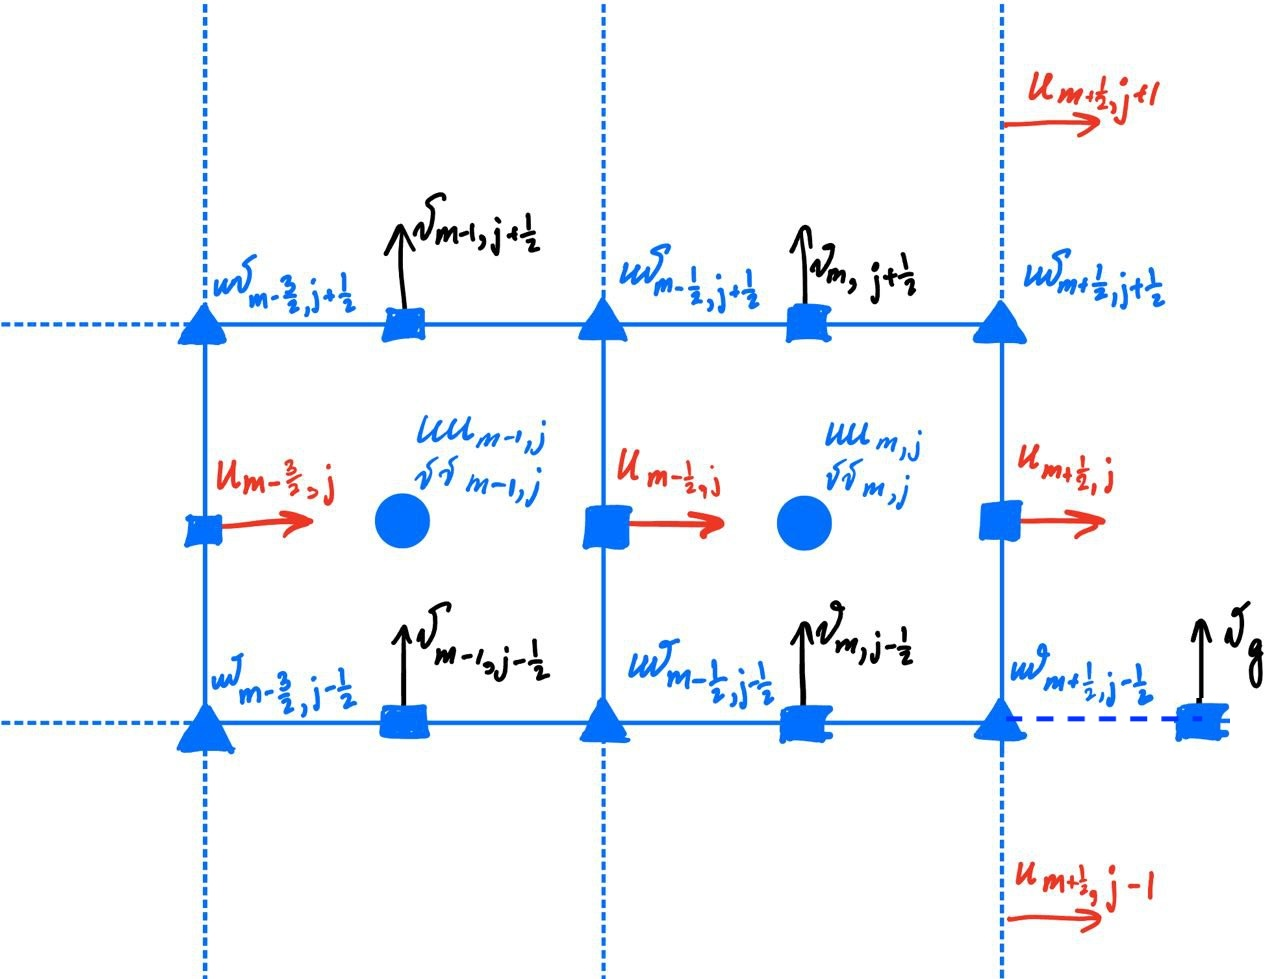
\includegraphics[width=0.45\paperwidth]{ADV-right}
  }
  \caption{$\hat{L}^u_{xx},\hat{L}^v_{xx}$ at the right boundary ($m=M$).}\label{fig:luxx-right}
\end{figure}
The rightmost unknown element of \cref{eqn:NSE-dsm-bl-system-schemes} in $x$ direction is $u^{n+1}_{M-\frac{1}{2},j}$ on \cref{fig:luxx-right}. Denote the vertical distances between three neighbouring $u$ components as $h_n$ and $h_s$, which stand for distances to the north $u^n_{M+\frac{1}{2},j+1}$ and south $u^{n}_{M+\frac{1}{2},j-1}$ neighbours from the $u^{n}_{M+\frac{1}{2},j}$ between them, while central $h_c$ is the average of $h_s$ and $h_n$.  To apply \cref{eqn:laplacian-discretization-non-uniform-dx} we need to express $u^{n+1}_{M+\frac{1}{2},j}$ using \cref{eqn:Jin-Braza-bc-transient}.
\begin{equation*}
\begin{gathered}
\frac{{u}^{n+1}_{M+\frac{1}{2},j}-{u}^n_{M+\frac{1}{2},j}}{\Delta t}
+\frac{u^n_{M+\frac{1}{2},j}}{2}
\left[
\left(
	\frac{u^{n+1}_{M+\frac{1}{2},j}-u^{n+1}_{M-\frac{1}{2},j}}{\Delta x_M}
\right)
+\left(
	\frac{u^{n}_{M+\frac{1}{2},j}-u^{n}_{M-\frac{1}{2},j}}{\Delta x_M}
\right)
\right] =\\
=\epsilon\left(\frac{1}{h_c h_s}u^{n}_{M+\frac{1}{2},j-1} - \frac{2}{h_n h_s}u^{n}_{M+\frac{1}{2},j} + \frac{1}{h_c h_n}u^n_{M+\frac{1}{2},j+1}\right)
\end{gathered}
\end{equation*}
leads to %%%%%%%%%%%%%%%%%
\begin{equation}\label[bc]{eqn:bc-u-right-long}
\begin{gathered}
\left(\frac{1}{\Delta t} + \frac{u^n_{M+\frac{1}{2},j}}{2\Delta x_M}\right){{u}^{n+1}_{M+\frac{1}{2},j}}
=
u^{n+1}_{M-\frac{1}{2},j}\frac{u^n_{M+\frac{1}{2},j}}{2\Delta x_M}-\\
-\frac{u^n_{M+\frac{1}{2},j}}{2}\frac{u^{n}_{M+\frac{1}{2},j}-u^{n}_{M-\frac{1}{2},j}}{\Delta x_M}
+\frac{{u}^n_{M+\frac{1}{2},j}}{\Delta t}
+\epsilon\left(\frac{1}{h_c h_s}u^{n}_{M+\frac{1}{2},j-1} - \frac{2}{h_n h_s}u^{n}_{M+\frac{1}{2},j} + \frac{1}{h_c h_n}u^n_{M+\frac{1}{2},j+1}\right).
\end{gathered}
\end{equation}
Note that $\left(\frac{1}{\Delta t} + \frac{u^n_{M+\frac{1}{2},j}}{2\Delta x_M}\right)$ can be made to never be zero regardless of the flow direction, hence dividing by it is allowed. The second line of fully discretized \cref{eqn:bc-u-right-long} is treated explicitly since we posses the flow data at time steps $n$ and earlier. Denote explicit terms as
\begin{equation*}
	bc_{u-\text{explicit}}^n=-\frac{u^n_{M+\frac{1}{2},j}}{2}\frac{u^{n}_{M+\frac{1}{2},j}-u^{n}_{M-\frac{1}{2},j}}{\Delta x_M}
+\frac{{u}^n_{M+\frac{1}{2},j}}{\Delta t}
+\epsilon\left(\frac{1}{h_c h_s}u^{n}_{M+\frac{1}{2},j-1} - \frac{2}{h_n h_s}u^{n}_{M+\frac{1}{2},j} + \frac{1}{h_c h_n}u^n_{M+\frac{1}{2},j+1}\right),
\end{equation*}
which simplifies \cref{eqn:bc-u-right-long} to 
\begin{equation}\label[bc]{eqn:bc-u-right}
\begin{gathered}
\left(\frac{1}{\Delta t} + \frac{u^n_{M+\frac{1}{2},j}}{2\Delta x_M}\right){{u}^{n+1}_{M+\frac{1}{2},j}}
=
u^{n+1}_{M-\frac{1}{2},j}\frac{u^n_{M+\frac{1}{2},j}}{2\Delta x_M}+bc_{u-\text{explicit}}^n.
\end{gathered}
\end{equation}

Next, we plug \cref{eqn:bc-u-right} into \cref{eqn:laplacian-discretization-non-uniform-dx}, which finally leads us to
\begin{equation}\label{eqn:luxx-right}
\begin{aligned}
	\left.\frac{\partial ^2 u}{\partial x^2}\right|_{M-\frac{1}{2},j}^{n+1}
	&=\frac{1}{h_c h_e}u^{n+1}_{M+\frac{1}{2},j} - \frac{2}{h_w h_e}u^{n+1}_{M-\frac{1}{2},j} + \frac{1}{h_c h_w}u^{n+1}_{M-\frac{1}{2}-1,j}+h.o.t.\\
	&=\frac{1}{h_c h_e}\frac{\left.u^{n+1}_{M-\frac{1}{2},j}\frac{u^n_{M+\frac{1}{2},j}}{2h_e}+bc_{u-\text{explicit}}^n\right.}{\left.\frac{1}{\Delta t} + \frac{u^n_{M+\frac{1}{2},j}}{2\Delta x_M}\right.}- \frac{2}{h_w h_e}u^{n+1}_{M-\frac{1}{2},j} + \frac{1}{h_c h_w}u^{n+1}_{M-\frac{1}{2}-1,j}+h.o.t.\\
	&=\left[ \frac{1}{h_c h_e}\left(\frac{u^n_{M+\frac{1}{2},j}}{2h_e\left[\frac{1}{\Delta t} + \frac{u^n_{M+\frac{1}{2},j}}{2\Delta x_M}\right]} \right) -\frac{2}{h_w h_e}\right]u^{n+1}_{M-\frac{1}{2},j} + \frac{1}{h_c h_w}u^{n+1}_{M-\frac{1}{2}-1,j} + \frac{bc_{u-\text{explicit}}^n}{h_c h_e\left(\frac{1}{\Delta t} + \frac{u^n_{M+\frac{1}{2},j}}{2\Delta x_M}\right)}+h.o.t..
\end{aligned}
\end{equation}

Condition for $v$ component is not as trivial as for $u$ since there is no $v$ directly at the boundary due to the staggered grid arrangement. We need to express $v_g=v_{M+1,j-\frac{1}{2}}$ in terms of the right-most unknown $v_{M,j-\frac{1}{2}}$ component for the diffusion operator. 
We can use more than one value of $v$ from inner part of the domain to express the ghost velocity outside. However, this will lead to change of non-diagonal elements in diffusion operator, which will cause Laplacian matrix to be asymmetric. Therefore, we are restricted to use the elements of the main diagonal to express the ghost velocities outside the computational domain. Hence, interpolation leads to
\begin{equation*}
	v_{\text{BC}}=v_{M+\frac{1}{2},j-\frac{1}{2}}=\frac{v_{M+1,j-\frac{1}{2}}+v_{M,j-\frac{1}{2}}}{2},
\end{equation*}
where $v_{M+1,j-\frac{1}{2}}$ is ghost component outside the domain. It is also possible to apply central difference to the advection terms at the boundary $\left( \frac{\partial v}{\partial x}\right)_{M+\frac{1}{2},j-\frac{1}{2}}=\frac{v_{M+1,j-\frac{1}{2}}-v_{M,j-\frac{1}{2}}}{\Delta x_{M+\frac{1}{2}}}$.

\cref{eqn:Jin-Braza-bc-transient} using the approximations from above can be rewritten for $v_{M+\frac{1}{2},j-\frac{1}{2}}$ component at the boundary as
\begin{equation*}
\begin{gathered}
\frac{{\left( \frac{v^{n+1}_{M+1,j-\frac{1}{2}}+v^{n+1}_{M,j-\frac{1}{2}}}{2}\right)}-\left( \frac{v^n_{M+1,j-\frac{1}{2}}+v^n_{M,j-\frac{1}{2}}}{2} \right) }{\Delta t}+\\
+\frac{\left.u^n_{M+\frac{1}{2},j-\frac{1}{2}}\right.}{2}
\left[
\left(
	\frac{v^{n+1}_{M+1,j-\frac{1}{2}}-v^{n+1}_{M,j-\frac{1}{2}}}{\Delta x_{M+\frac{1}{2}}}
\right) \right.
+\left.\left(
	\frac{v^{n}_{M+1,j-\frac{1}{2}}-v^{n}_{M,j-\frac{1}{2}}}{\Delta x_{M+\frac{1}{2}}}
\right)
\right]= \\
=\epsilon\left[\frac{1}{h_c h_s}\left(\frac{v^{n}_{M+1,j-\frac{1}{2}-1}+v^{n}_{M,j-\frac{1}{2}-1}}{2} \right) - \frac{2}{h_n h_s}\left(\frac{v^{n}_{M+1,j-\frac{1}{2}}+v^{n}_{M,j-\frac{1}{2}}}{2} \right) + \frac{1}{h_c h_n}\left(\frac{v^{n}_{M+1,j+\frac{1}{2}}+v^{n}_{M,j+\frac{1}{2}}}{2} \right)\right],
\end{gathered}
\end{equation*}
which is used to express ghost velocity $v^{n+1}_{M+1,j-\frac{1}{2}}$ after rearranging
\begin{equation}\label[bc]{eqn:bc-v-right-long}
\begin{gathered}
\left( \frac{1}{2\Delta t} + \frac{u^n_{M+\frac{1}{2},j-\frac{1}{2}}}{2\Delta x_{M+\frac{1}{2}}}\right) v^{n+1}_{M+1,j-\frac{1}{2}}
=\left( -\frac{1}{2\Delta t}+\frac{u^n_{M+\frac{1}{2},j-\frac{1}{2}}}{2\Delta x_{M+\frac{1}{2}}} \right)v^{n+1}_{M,j-\frac{1}{2}}+\\
+\left( \frac{v^n_{M+1,j-\frac{1}{2}}+v^n_{M,j-\frac{1}{2}}}{2\Delta t} \right)
+ \frac{\left.u^n_{M+\frac{1}{2},j-\frac{1}{2}}\right.}{2}\left(\frac{v^{n}_{M+1,j-\frac{1}{2}}-v^{n}_{M,j-\frac{1}{2}}}{\Delta x_{M+\frac{1}{2}}}\right)+\\
+\epsilon\left[\frac{1}{h_c h_s}\left(\frac{v^{n}_{M+1,j-\frac{1}{2}-1}+v^{n}_{M,j-\frac{1}{2}-1}}{2} \right) - \frac{2}{h_n h_s}\left(\frac{v^{n}_{M+1,j-\frac{1}{2}}+v^{n}_{M,j-\frac{1}{2}}}{2} \right) + \frac{1}{h_c h_n}\left(\frac{v^{n}_{M+1,j+\frac{1}{2}}+v^{n}_{M,j+\frac{1}{2}}}{2} \right)\right].
\end{gathered}
\end{equation}
Let us denote explicit terms from last two rows as
\begin{equation*}
\begin{gathered}
	bc_{v-\text{explicit}}^n=\left( \frac{v^n_{M+1,j-\frac{1}{2}}+v^n_{M,j-\frac{1}{2}}}{2\Delta t} \right)
+ \frac{\left.u^n_{M+\frac{1}{2},j-\frac{1}{2}}\right.}{2}\left(\frac{v^{n}_{M+1,j-\frac{1}{2}}-v^{n}_{M,j-\frac{1}{2}}}{\Delta x_{M+\frac{1}{2}}}\right)+\\
+\epsilon\left[\frac{1}{h_c h_s}\left(\frac{v^{n}_{M+1,j-\frac{1}{2}-1}+v^{n}_{M,j-\frac{1}{2}-1}}{2} \right) - \frac{2}{h_n h_s}\left(\frac{v^{n}_{M+1,j-\frac{1}{2}}+v^{n}_{M,j-\frac{1}{2}}}{2} \right) + \frac{1}{h_c h_n}\left(\frac{v^{n}_{M+1,j+\frac{1}{2}}+v^{n}_{M,j+\frac{1}{2}}}{2} \right)\right].
\end{gathered}
\end{equation*}
Then \cref{eqn:bc-v-right-long} simplifies to
\begin{equation}\label[bc]{eqn:bc-v-right}
\begin{gathered}
\left( \frac{1}{2\Delta t} + \frac{u^n_{M+\frac{1}{2},j-\frac{1}{2}}}{2\Delta x_{M+\frac{1}{2}}}\right) v^{n+1}_{M+1,j-\frac{1}{2}}
=\left( -\frac{1}{2\Delta t}+\frac{u^n_{M+\frac{1}{2},j-\frac{1}{2}}}{2\Delta x_{M+\frac{1}{2}}} \right)v^{n+1}_{M,j-\frac{1}{2}}+bc_{v-\text{explicit}}^n.
\end{gathered}
\end{equation}

The ultimate step is to plug \cref{eqn:bc-v-right} into \cref{eqn:laplacian-discretization-non-uniform-dx} which will result in diffusion approximation of $v$ in $x$ direction of the right-most unknown component
\begin{equation}\label{{eqn:lvxx-right}}
\begin{aligned}
	\left.\frac{\partial ^2 v}{\partial x^2}\right|_{M,j-\frac{1}{2}}^{n+1}
	&=\frac{1}{h_c h_e}v^{n+1}_{M+1,j-\frac{1}{2}} - \frac{2}{h_w h_e}v^{n+1}_{M,j-\frac{1}{2}} + \frac{1}{h_c h_w}v^{n+1}_{M-1,j-\frac{1}{2}}+h.o.t.\\
	&=\frac{1}{h_c h_e}\left[\frac{\left( -\frac{1}{2\Delta t}+\frac{u^n_{M+\frac{1}{2},j-\frac{1}{2}}}{2h_e} \right)v^{n+1}_{M,j-\frac{1}{2}}+bc_{v-\text{explicit}}^n}{\left. \frac{1}{2\Delta t} + \frac{u^n_{M+\frac{1}{2},j-\frac{1}{2}}}{2h_e}\right.}\right]- \frac{2}{h_w h_e}v^{n+1}_{M,j-\frac{1}{2}} + \frac{1}{h_c h_w}v^{n+1}_{M-1,j-\frac{1}{2}}+h.o.t.\\
	&=\left[ \frac{1}{h_c h_e}\left(\frac{\left. -\frac{1}{2\Delta t}+\frac{u^n_{M+\frac{1}{2},j-\frac{1}{2}}}{2h_e} \right.}{\left. \frac{1}{2\Delta t} + \frac{u^n_{M+\frac{1}{2},j-\frac{1}{2}}}{2h_e}\right.} \right) -\frac{2}{h_w h_e}\right]v^{n+1}_{M,j-\frac{1}{2}} + \frac{1}{h_c h_w}v^{n+1}_{M-1,j-\frac{1}{2}} + \frac{bc_{v-\text{explicit}}^n}{h_c h_e\left( \frac{1}{2\Delta t} + \frac{u^n_{M+\frac{1}{2},j-\frac{1}{2}}}{2h_e}\right)}+h.o.t..
\end{aligned}
\end{equation}

Let us now try to apply \cref{eqn:Jin-Braza-bc-transient-consistent} which is consistent with schemes for the inner part to the boundary values at the outlet
\begin{equation*}
\begin{gathered}
\frac{{u}^{n+1}_{M+\frac{1}{2},j}-{u}_{M+\frac{1}{2},j}^n}{\Delta t}+\left[\frac{3}{2}{u_{M+\frac{1}{2},j}^n}\left(\frac{\partial {u}}{\partial x}\right)^{n}_{M+\frac{1}{2},j}-\frac{1}{2}{u_{M+\frac{1}{2},j}^{n-1}}\left(\frac{\partial {u}}{\partial x}\right)^{n-1}_{M+\frac{1}{2},j}\right]\\
=\epsilon\left[\left(\frac{\partial^2 {u}}{\partial y^2}\right)^{n+1}_{M+\frac{1}{2},j}+\left(\frac{\partial^2 {u}}{\partial y^2}\right)^{n}_{M+\frac{1}{2},j}\right].
\end{gathered}
\end{equation*}
The above equation after discretizing spatially becomes
\begin{equation}\label[bc]{eqn:Jin-Braza-bc-full-consistent}
\begin{gathered}
\frac{\epsilon}{h_c h_n}u^{n+1}_{M+\frac{1}{2},j+1} - \left(\frac{2\epsilon}{h_s h_n}-\frac{1}{\Delta t}\right)u^{n+1}_{M+\frac{1}{2},j} + \frac{\epsilon}{h_c h_s}u^{n+1}_{M+\frac{1}{2},j-1}\\
=-\frac{{u}_{M+\frac{1}{2},j}^n}{\Delta t}+\left[\frac{3}{2}{u_{M+\frac{1}{2},j}^n}\left(\frac{u_{M+\frac{1}{2},j}^n-u_{M-\frac{1}{2},j}^n}{\Delta x_M}\right)-\frac{1}{2}{u_{M+\frac{1}{2},j}^{n-1}}\left(\frac{u_{M+\frac{1}{2},j}^{n-1}-u_{M-\frac{1}{2},j}^{n-1}}{\Delta x_M}\right)\right]\\
-\left[\frac{\epsilon}{h_c h_n}u^{n}_{M+\frac{1}{2},j+1}-\frac{2\epsilon}{h_s h_n}u^{n}_{M+\frac{1}{2},j} + \frac{\epsilon}{h_c h_s}u^{n}_{M+\frac{1}{2},j-1}\right].
\end{gathered}
\end{equation}

The fully discretized \cref{eqn:Jin-Braza-bc-full-consistent} from above is a system of linear equations at time step $n+1$ and only has to be solved for the outlet boundary values of $u$. We know both topmost velocity $u_{\text{top}}=u_{\text{freestream}}$ and bottommost $u_{\text{bot}}=u_{\text{wall}}$ which play roles of boundary values for this system of equations. However, there is an issue that no velocity values at time step $n+1$ are passed from the inner part of the domain, the whole equation is self-sufficient and takes only the inner data from previous time steps $n$ and $n-1$. Thus, \cref{eqn:Jin-Braza-bc-full-consistent} behaves as an independent equation from main \cref{eqn:NSE-dsm-bl-system-schemes}.


%%%%%%%%%%%%%%%%%%%%%%%%%%%%%%%%%%%%%%%%%%%%%%%%%%%%%%%%%%%%%%%%%%%%%%%%%%%%%%%%%%%%%%%%%%%%%%%%
\subsection{Advection at the right boundary using ABC}\label{subsec:advection-ABC}
%\textbf{Advection at the right boundary.}
\begin{figure}[H] % here, bottom, top
  \centering{
  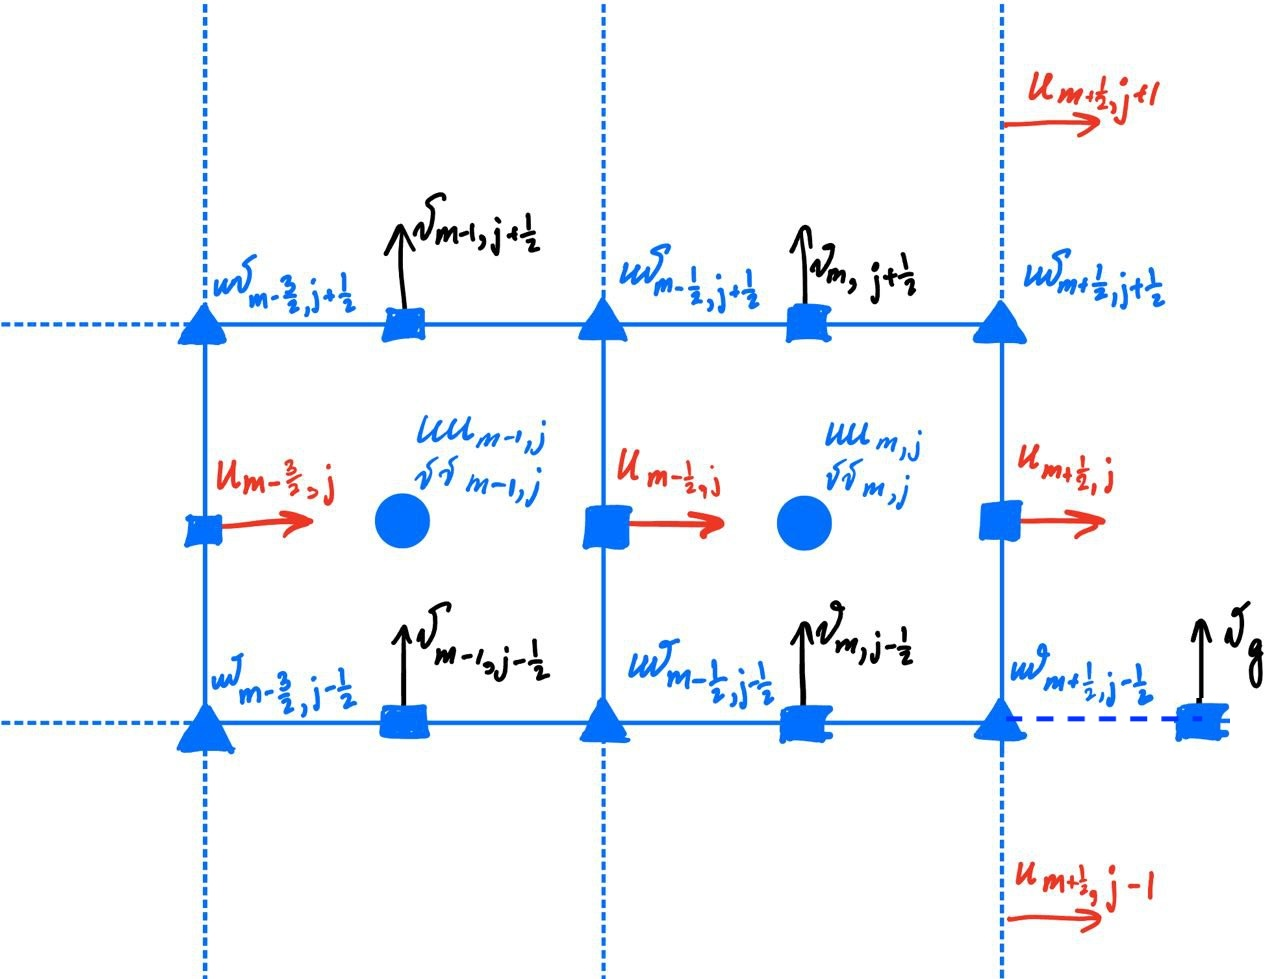
\includegraphics[width=0.45\paperwidth]{ADV-right}
  }
  \caption{Right boundary advection.}\label{fig:ADV-right}
\end{figure}
\cref{eqn:bc-u-right} rewritten for the time step $n$ is
\begin{equation*}
\begin{gathered}
{{u}^{n}_{M+\frac{1}{2},j}}\left(\frac{1}{\Delta t} + \frac{u^{n-1}_{M+\frac{1}{2},j}}{2\Delta x_M}\right)
=
u^{n}_{M-\frac{1}{2},j}\frac{u^{n-1}_{M+\frac{1}{2},j}}{2\Delta x_M}+bc_e^{n-1}.
\end{gathered}
\end{equation*}
This can be used to obtain the value $u^{n}_{M+\frac{1}{2},j}$ at the right boundary. Then we use the \cref{eqn:adv-inner} for inner part as now all the necessary values are known. Similarly, \cref{eqn:bc-v-right} at time step $n$
\begin{equation*}
\begin{gathered}
\left( \frac{1}{2\Delta t} + \frac{u^n_{M+\frac{1}{2},j-\frac{1}{2}}}{2\Delta x_{M+\frac{1}{2}}}\right) v^{n}_{M+1,j-\frac{1}{2}}
=\left( -\frac{1}{2\Delta t}+\frac{u^n_{M+\frac{1}{2},j-\frac{1}{2}}}{2\Delta x_{M+\frac{1}{2}}} \right)v^{n}_{M,j-\frac{1}{2}}+bc_{ve}^{n-1}
\end{gathered}
\end{equation*}
is used to express ghost velocity $v^{n}_{M+1,j-\frac{1}{2}}$, which we use to compute \cref{eqn:adv-inner} for inner part.



\section{Symmetrization}\label{sec:symmetrization}

The most effective methods for solving systems of linear equations often work optimally with symmetric matrices, making symmetry a desirable property. In order to achieve a symmetric system, we introduce two matrices - the diagonal scaling matrix $\hat{M}$ and the diagonal flux matrix $R$. These matrices are defined as
\begin{align*}
R &\equiv\left[\begin{array}{cc}
\Delta y_j & 0 \\
0 & \Delta x_i
\end{array}\right], \\
\quad \hat{M} & \equiv\left[\begin{array}{cc}
\frac{1}{2}\left(\Delta x_i+\Delta x_{i-1}\right) & 0 \\
0 & \frac{1}{2}\left(\Delta y_j+\Delta y_{j-1}\right)
\end{array}\right].
\end{align*}
 % and $\hat{D}R^{-1}=-(\hat{M}\hat{G})^T$. I THINK THIS WRONG BUT WRITTEN IN TAIRA DISSERTATION ON PAGE 101.

%The only matrix which can be asymmetric in~\cref{eqn:NSE-dsm-bl-system-schemes} is a Laplacian if the grid is non-uniform. In order to get a symmetric diffusion matrix we need to move to the new variables. 
Define matrices 
\begin{equation*}
\begin{aligned}
	\Delta y_j&=\text{diag}([\underbrace{\Delta y_1; \Delta y_1; \dotsc;\Delta y_1}_{M-1\text{ times}}; \underbrace{\Delta y_2; \Delta y_2; \dotsc;\Delta y_2}_{M-1\text{ times}};\dotsc;\underbrace{\Delta y_N; \Delta y_N; \dotsc;\Delta y_N}_{M-1\text{ times}}]),\\
	\Delta x_i&=\text{diag}([\underbrace{\Delta x_1; \Delta x_2;\dotsc\Delta x_M;\Delta x_1; \Delta x_2;\dotsc\Delta x_M; \dotsc;\Delta x_1; \Delta x_2;\dotsc;\Delta x_M}_{N-1\text{ blocks of } 1,\dotsc,M}]),
\end{aligned}
\end{equation*}
which are then combined into
\begin{equation*}
R =\left[\begin{array}{cc}
\Delta y_j & 0 \\
0 & \Delta x_i
\end{array}\right].
\end{equation*}

By moving to new variable ${q} = R\boldsymbol{v}$, we use matrix $R$, which inverse $R^{-1}$ performs half of the symmetrization process for $\hat{L}$. 
Here, $R$ is a diagonal matrix of size $(M-1)N\times M(N-1)$.  Using the $R$ matrix we can express mass flux $q^{n+1}=R\boldsymbol{v}^{n+1}\implies \boldsymbol{v}^{n+1}=R^{-1}q^{n+1}$. It is required that the difference matrices cancel out $\frac{x_{i+1}-x_{i-1}}{2}$ central term in diffusion discretization to make Laplacian partially symmetric. Define the elements of diagonal mass matrix as
\begin{equation*}
{\Delta x_i+\Delta x_{i-1}} = \text{diag}[\underbrace{\Delta x_2+\Delta x_1; \Delta x_3+\Delta x_2; \dotsc ;\Delta x_{M}+\Delta x_{M-1}; ...;\Delta x_2+\Delta x_1; \Delta x_3+\Delta x_2; \dotsc \Delta x_{M}+\Delta x_{M}}_{N\text{ times for each block of } \Delta x_2+\Delta x_1\text{ to }\Delta x_{M}+\Delta x_{M-1}}]
\end{equation*}
and
\begin{equation*}
{\Delta y_j+\Delta y_{j-1}} = \text{diag}[\underbrace{\Delta y_2+\Delta y_1;  \dotsc \Delta y_2+\Delta y_1;}_{M\text{ times}} \underbrace{\Delta y_3+\Delta y_2; \dotsc \Delta y_3+\Delta y_2;}_{M\text{ times}} \underbrace{\Delta y_N+\Delta y_{N-1}\dotsc \Delta y_N+\Delta y_{N-1}}_{M\text{ times}}],	
\end{equation*}
which are then combined into
\begin{equation*}
\hat{M} =\left[\begin{array}{cc}
\frac{1}{2}\left(\Delta x_i+\Delta x_{i-1}\right) & 0 \\
0 & \frac{1}{2}\left(\Delta y_j+\Delta y_{j-1}\right)
\end{array}\right],
\end{equation*}
which both removes the $M^{-1}$ in $\hat{G}=\hat{M}^{-1}G$ if left multiplied and completes the symmetrization process of $\hat{L}$.

The identity ${q}=R\boldsymbol{v}$ implies $\boldsymbol{v}=R^{-1}{q}$, therefore, Laplacian matrix multiplied by the velocity vector is
$$\hat{L}\boldsymbol{v}= \hat{L}R^{-1}{q},$$ 
premultiplying by $\hat M$ we obtain
$$\hat M\hat{L}R^{-1}{q},$$ 
where $\hat M L R^{-1}$ is symmetric by construction, hence, $\hat M\hat{A}R^{-1}=\hat M (\frac{1}{\Delta t}\mathbf{I}-\frac{1}{2}L) R^{-1}$ is also symmetric.  

Using the above transformations we can modify \cref{eqn:NSE-dsm-bl-system-nonint}
%\begin{equation*}
%\left[\begin{array}{ccc}
%\hat{A} & \hat{G} \\
%\hat{D} & 0 
%\end{array}\right]\left(\begin{array}{c}
%\boldsymbol{v}^{n+1} \\
%p
%\end{array}\right)=\left(\begin{array}{c}
%\hat{r}^n \\
%0 
%\end{array}\right)+\left(\begin{array}{c}
%\widehat{bc}_1 \\
%\widehat{bc}_2 
%\end{array}\right)
%\end{equation*}
into 
\begin{equation*}
\left[\begin{array}{cc}
\hat{M}\hat{A}R^{-1} & \hat{M}\hat{G} \\
\hat{D}R^{-1} & 0
\end{array}\right]\left(\begin{array}{c}
q^{n+1} \\
p^{n+1}
\end{array}\right)=\left(\begin{array}{c}
\hat{M}\hat{r}^n \\
0
\end{array}\right)+\left(\begin{array}{c}
\hat{M}\widehat{b c}_1 \\
\widehat{b c}_2
\end{array}\right),
\end{equation*}
which can be rewritten as 
\begin{equation}\label[system]{eqn:nse-normalized}
\left[\begin{array}{cc}
A & G \\
D & 0
\end{array}\right]\left(\begin{array}{c}
q^{n+1} \\
p^{n+1}
\end{array}\right)=\left(\begin{array}{c}
r^n \\
0
\end{array}\right)+\left(\begin{array}{c}
{b c}_1 \\
{b c}_2
\end{array}\right),
\end{equation}
where $A=\hat{M}\hat{A}R^{-1}=\frac{1}{\Delta t}\hat{M}R^{-1}-\frac{1}{2}\hat{M}\hat{L}R^{-1}$ is symmetric and $\hat{G}=\hat{M}^{-1}G$ according to \cref{eqn:gradient-matrix}. It is also possible to transform the divergence operator $\hat{D}$ with non-integer coefficients into $D$ with integer coefficients in continuity part of \cref{eqn:nse-normalized} using  \cref{eqn:divergence-matrix}. Multiplying both sides of continuity equation by $\Delta _{xy}$ matrix from \cref{eqn:delta-xy} leads to 
\begin{align*}
	\hat{D}\boldsymbol{v}^{n+1}&= \hat{bc}_2\notag\\
	\left(\Delta_{xy} \right)\hat{D}\boldsymbol{v}^{n+1}&=\left ( \Delta_{xy}\right ) \hat{bc}_2\notag\\
	\left(\Delta_{xy}\right)\frac{1}{\Delta _{xy}}{D}R\boldsymbol{v}^{n+1}&=\left ( \Delta_{xy}\right ) \hat{bc}_2\notag\\
	\left(\Delta_{xy}\right)\frac{1}{\Delta_{xy}}{D}q^{n+1}&=\left ( \Delta_{xy}\right ) \hat{bc}_2\notag\\
	D{q}^{n+1}&=bc_2.
\end{align*}


	\section{Vorticity-stream function formulation}\label{sec:vorticity-streamfunction}
	The algorithm to be used is a combination of classical formulation as in \cref{eqs:NSE} and vorticity-stream function \cref{eqn:transport-vorticity,eqn:vorticity-stream}.
	Consider:
	
	\begin{enumerate}
	\item	

	Stream function $\psi(x,y,t):\boldsymbol{v}=\nabla \times \psi$ of an incompressible two-dimensional flow:
	\begin{equation}
	\label{eqn:streamfunction}
		u = \frac{\partial \psi}{\partial y},\quad v=-\frac{\partial \psi}{\partial x},
	\end{equation}
	where $\boldsymbol{v}=(u,v)$.
	
	The velocity vector at every point of space and every moment of time is tangential to the line $\psi = const$ and such lines represent the streamlines of the flow. 
	\item
	
	Vorticity $\omega = \nabla \times \boldsymbol{v}$, in two-dimensional case (x-y-plane) the only non-zero component of $\omega$ is $z$, which leads to
	\begin{equation}
	\label{eqn:vorticity}
		\omega=\frac{\partial v}{\partial x} - \frac{\partial u}{\partial y}.
	\end{equation}
	\end{enumerate}
	
	Importantly, continuity \cref{eqn:continuity} is satisfied immediately by taking spatial derivatives of stream function \cref{eqn:streamfunction} components and adding them up. The governing \cref{eqs:NSE} can now be transformed. The new equations are changed to the following:
	\begin{enumerate}
		\item 
			Transport equation for vorticity.
			
			Application of $(\nabla \times)$ to momentum and taking into account continuity \cref{eqn:continuity} together with the fact
			\begin{equation*}
				\frac{\partial}{\partial y}\left(\frac{\partial p}{\partial x}\right) - 
				\frac{\partial}{\partial x}\left(\frac{\partial p}{\partial y}\right)=0
			\end{equation*}
			results in
			\begin{equation}
			\label{eqn:transport-vorticity}
				\boxed{
				\frac{\partial\omega}{\partial t} 
				+ u \frac{\partial\omega}{\partial x} 
				+ v\frac{\partial\omega}{\partial y} 
				= \epsilon \left(\frac{\partial ^2 \omega}{\partial x^2} 
				+ \frac{\partial^2 \omega}{\partial y^2} \right).
				}
			\end{equation}
			
		\item 
		Vorticity-Stream function equation.
		
		After substituting stream function \cref{eqn:streamfunction} into vorticity \cref{eqn:vorticity} we obtain
		\begin{equation}
			\label{eqn:vorticity-stream}
			\boxed{\nabla ^2 \psi = -\omega.}
		\end{equation}	
	\end{enumerate}
	
	These two equations above form a coupled system, and the pressure field does not explicitly appear in neither \cref{eqn:transport-vorticity} nor \cref{eqn:vorticity-stream} and, in principle, is not needed in the solution.
	
	The system (\cref{eqn:transport-vorticity,eqn:vorticity-stream}) requires boundary conditions on $\psi$ and $\omega$. For the stream function, imposing physically plausible conditions is not difficult. One has to write the proper boundary conditions for the velocity components and use vorticity \cref{eqn:vorticity} to represent them as conditions for $\psi$ and its derivatives. The situation is more difficult in the case of vorticity. There are no natural boundary conditions on $\omega$, but they can be derived from the conditions on $\psi$ by application of the \cref{eqn:vorticity-stream} at the boundary. The process of finding boundary conditions of $\omega$ typically results in expressions containing second derivatives, therefore, special numerical treatment is required.
	
	To overcome the issue above we first apply boundary conditions in terms of velocity and pressure and keep them explicit as in \cref{eqn:NSE-dsm-bl-system-schemes}. Our goal is to modify the implicit (left) part of \cref{eqn:NSE-dsm-bl-system-schemes} by transforming it into vorticity transport \cref{eqn:transport-vorticity} together with vorticity stream function substitution \cref{eqn:vorticity-stream} which results in 
	\begin{equation}
	\label{eqn:biharmonic-streamfunction}
		\boxed{
		\frac{\partial\nabla ^2 \psi}{\partial t} 
		-\Delta ^2 \psi=-\operatorname{RHS_{\boldsymbol{v},p}},
		}
	\end{equation}
where the right hand side terms were initially stated in terms of $\boldsymbol{v},p$ and transformed using the same operations as the left hand side of \cref{eqn:biharmonic-streamfunction}.

\section{Nullspace method and pressure elimination}\label{sec:nullspace-method}

The goal of this subsection is to show how unknown pressure variables can be eliminated from \cref{eqn:nse-normalized}. Publications of Chang~\cite{Chang:2002} and Hall~\cite{Hall:1980} use the idea that in \cref{eqn:nse-normalized} matrix $D$ is wider than tall for grids larger than $2\times 2$, hence it defines a nullspace. The nullspace of matrix $D$ is the set of all solutions to the homogeneous linear system $Dx = 0$, where $x$ is a vector in the null space of $D$. Let $C$ be the nullspace matrix containing such vectors $x$. 

The number of rows in the nullspace $C$ is equal to the number of faces with unknown velocities ($N_f$). In two dimensions $C$ has $N_n$ columns, which is equal to the number of nodes in the grid, whereas in three dimensions the nullspace has $N_e$ columns being the number of edges. 

In the two-dimensional case, the matrix $C$ has two non-zero elements in each row, which are $+1$ and $-1$. The $+1$ value corresponds to the node $90^\circ$ from the normal velocity vector, whereas $-1$ corresponds to the node $-90^\circ$ from the normal velocity vector.  For three dimensional case see Chang ~\cite{Chang:2002}.

%A more intuitive way of constructing the matrix $C$ relies on the usage of a counterclockwise vorticity around the nodes inside the domain and the boundary if such nodes have adjacent velocities from $\boldsymbol{v}$. In the case of the open boundary vortices around the nodes belonging to the open segment are taken into consideration. If the direction of the velocity vector on the adjacent face matches the direction of the vorticity then $+1$ is put into the corresponding row, $-1$ in case of the opposite directions of the velocity and vorticity. The matrix $C$ has the dimension of unknown velocities times the number of nodes around which these velocities revolve. Figure~\ref{fig:DC} shows matrices $D$ and $C$ for a $4\times4$ grid case with an open boundary on the right side of the domain. Yellow squares indicate $+1$, whereas blue squares correspond to $-1$ entries. The desired product then becomes $DC=0$ and since $D=-G^T$ we also have $(DC)^T=C^TD^T=-C^TG=0$. 
\begin{figure}[H] % here, bottom, top
  \centering{
  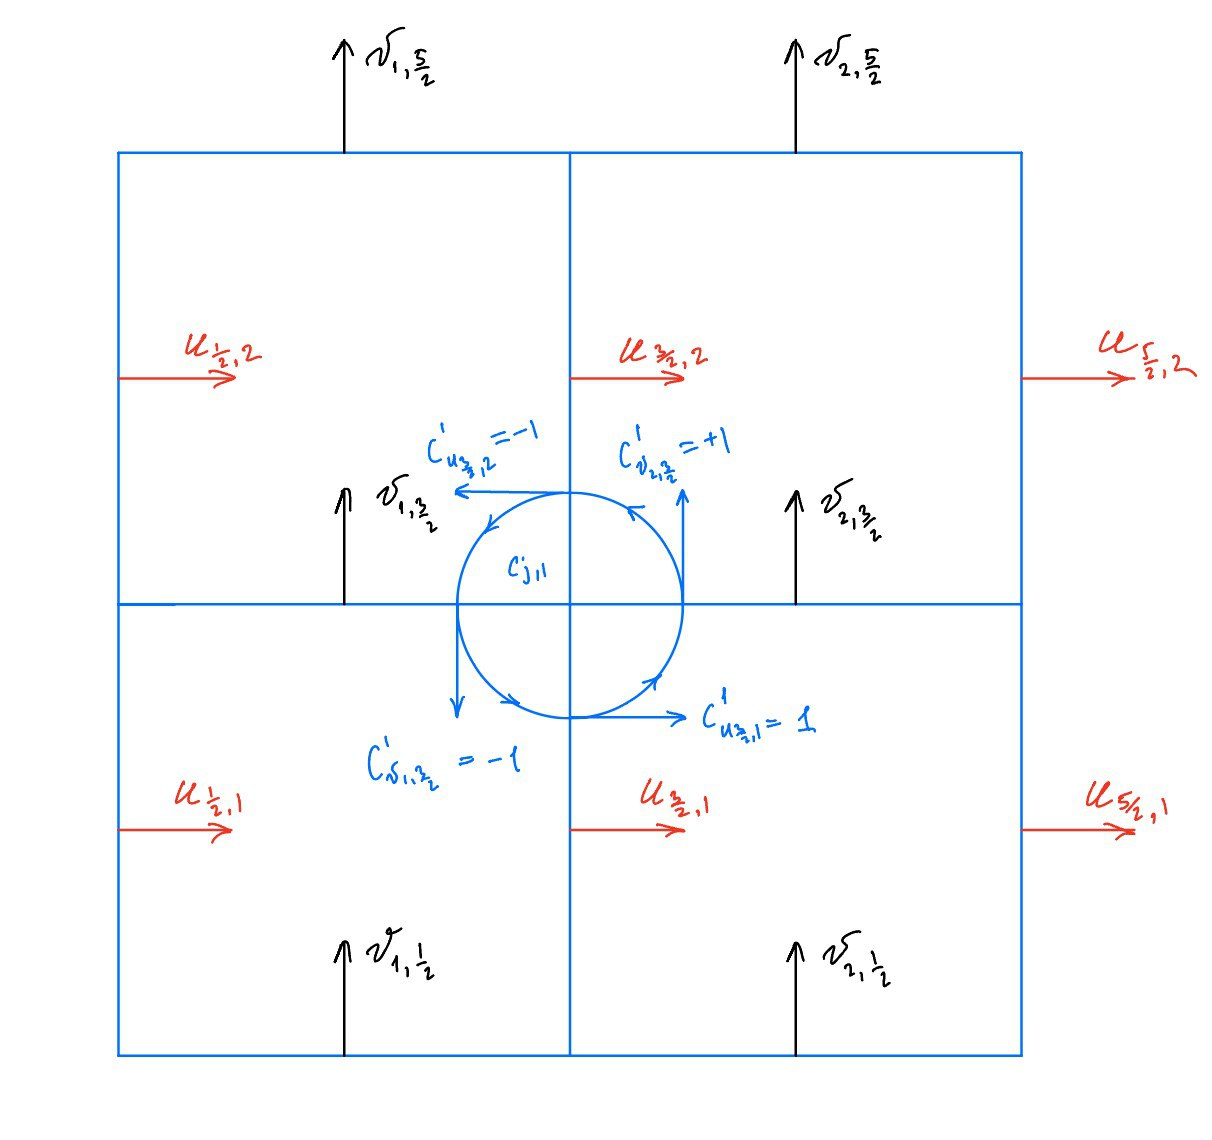
\includegraphics[width=0.40\paperwidth]{C-example-2x2}
  }
  \caption{$2\times 2$ example for $C$ matrix.}\label{fig:C-example-2x2}
\end{figure}
A more intuitive way of constructing the matrix $C$ relies on the utilization of counterclockwise vorticity around the nodes within the domain (\cref{fig:C-example-2x2}). If the direction of the velocity vector on the adjacent face aligns with the vorticity's direction, +1 is assigned to the corresponding row; conversely, -1 is assigned in the case of opposite directions of velocity and vorticity. After applying the above procedure we obtain
\begin{equation*}
  C = 
  \begin{bmatrix*}[r]
  1		\\
%  0		\\
  -1	\\
%  0		\\
  -1	\\
  1		\\
\end{bmatrix*}.
\end{equation*}

\begin{figure}[H]
\begin{center}
  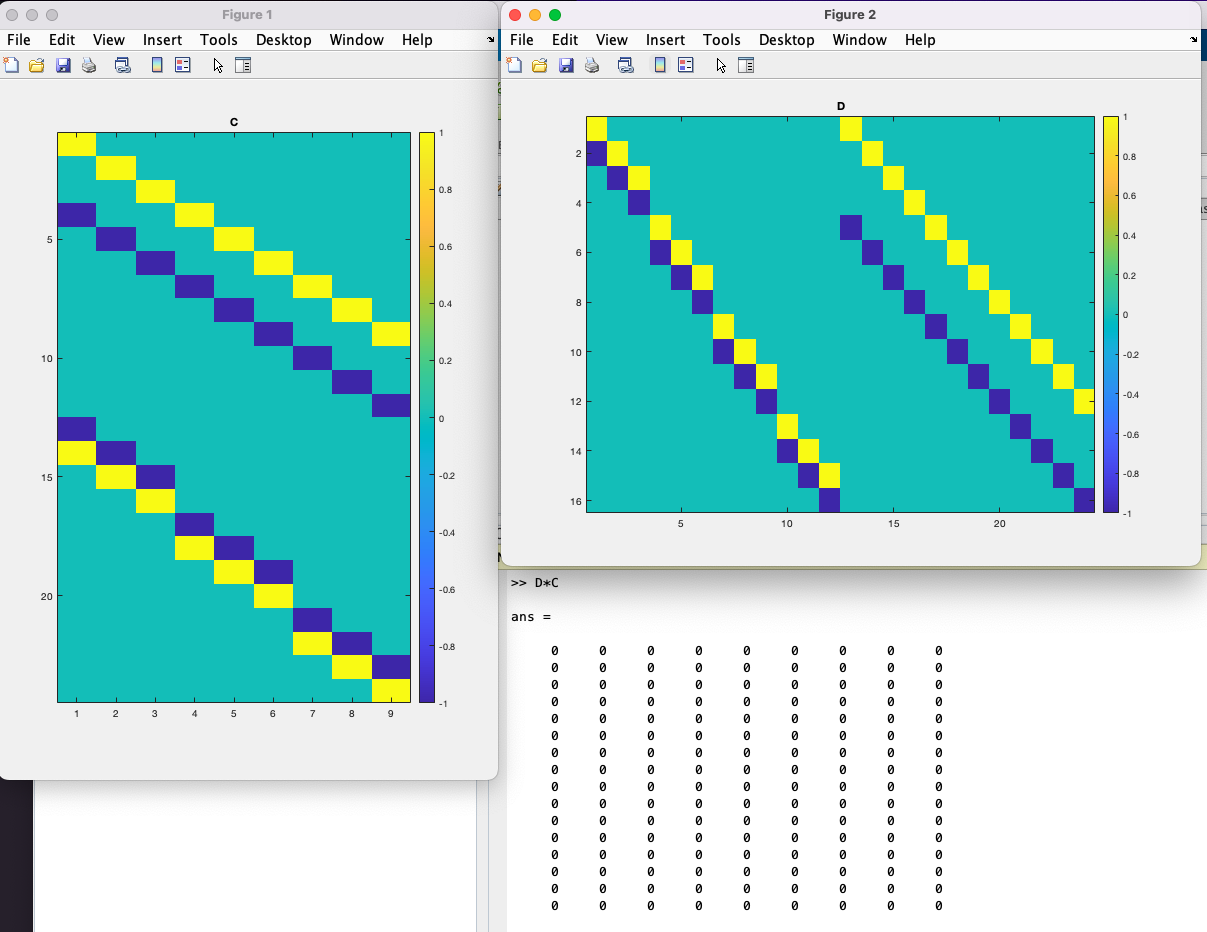
\includegraphics[width=0.75\textwidth]{Figures/D-C-DC}
\end{center}
\caption{Divergence and Curl matrices.}
\label{fig:DC}
\end{figure}
The matrix $C$ has dimensions corresponding to unknown velocities times the number of nodes around which these velocities revolve. Figure~\ref{fig:DC} illustrates matrices $D$ and $C$ for a $4\times4$ grid with an open boundary on the right side of the domain. 
%Yellow squares represent $+1$ entries, while blue squares correspond to $-1$. 
The desired product then becomes $DC=0$. $D=-G^T$ (derived in \cref{subsec:divergence,subsec:gradient}) leads to important property $(DC)^T=C^TD^T=-C^TG=0$. Premultiplying momentum equation in \cref{eqn:nse-normalized} by $C^T$ creates $C^TGp=0$ term, which completely eliminates the pressure from our system.

In order to make use of efficient solvers, the matrix $C^TA$ can be made symmetric if multiplied by $C$ from the right. We use the property of product $C^TC=L$ being symmetric Laplacian and $C^TLC=L^2$ being symmetric biharmonic operator as in \cref{eqn:biharmonic-streamfunction}. 
%\cref{eqn:vorticity-stream}
%\cref{eqn:vorticity-stream}
%\cref{eqn:vorticity-stream}
%\cref{eqn:vorticity-stream}
%\cref{eqn:vorticity-stream}
%\cref{eqn:vorticity-stream}
%\cref{eqn:vorticity-stream}
%\cref{eqn:vorticity-stream}
%\cref{eqn:vorticity-stream}
%\cref{eqn:vorticity-stream}
Hence, the final chord of this method is the introduction of new variable called discrete streamfunction $\psi:q_h=C\psi$, where $q_h$ is a homogeneous solution to the \cref{eqn:nse-normalized} and $q=q_h+q_p$ decomposition is discussed in the following \cref{sec:algorithm}.



\section{Resulting algorithm}\label{sec:algorithm}

Let us consider the solution to discretized \cref{eqn:nse-normalized}
\begin{equation*}
	q^{n+1}=q^{n+1}_p+q^{n+1}_h,
\end{equation*}
where $q^{n+1}_h$ is a solution to homogeneous continuity equation 
\begin{equation}\label{eqn:discrete-homogeneous-continuity}
	Dq^{n+1}_h=0,
\end{equation}
and $q^{n+1}_p$ is a particular solution to a non-homogeneous continuity equation
\begin{equation}\label{eqn:discrete-non-homogeneous-continuity}
	Dq^{n+1}_p=bc_2.
\end{equation}

%%%%%%%%%%%%%%
% REMOVE SOURCE TERM BELOW? S_1
%%%%%%%%%%%%%%

We assume that momentum equation from \cref{eqn:nse-normalized} modified to streamfunction \cref{eqn:biharmonic-streamfunction} with biharmonic operator satisfies homogeneous \cref{eqn:discrete-homogeneous-continuity} as in Colonius-Taira \cite{Colonius:2008}. 
The difference between \cite{Colonius:2008} and the method described below lies in boundary conditions. Colonius and Taira used homogeneous conditions at all boundaries (e.g. $\frac{\partial u}{\partial x}=0$ at inlet-outlet). 
Therefore, it was not needed for them to solve an additional non-homogeneous \cref{eqn:discrete-non-homogeneous-continuity}, whereas, in our problem statement such equation has to be solved due to non-zero Dirichlet and Neumann boundary conditions.
Thus, the resulting algorithm for discrete Navier-Stokes \cref{eqn:nse-normalized} can be described as follows:
\begin{enumerate}
	\item Construct matrix $C$, such that $DC=0$ and $q_h=C\psi$.\label[step]{step:1}
	\item Rewrite $q^{n+1}=q^{n+1}_p+q^{n+1}_h$.\label[step]{step:2}
	\item Find $q^{n+1}_p$ from the non-homogeneous continuity \cref{eqn:discrete-non-homogeneous-continuity} using the method described in next \cref{sec:continuity-particular-solution}.\label[step]{step:3}
	\item Split the solution $q^{n+1}$ into homogeneous and particular, then eliminate the pressure terms in the momentum equation.\label[step]{step:4}
		\begin{align}
			Aq^{n+1}&=-Gp^{n+1}+bc_1,\notag\\
			A(q^{n+1}_h+q^{n+1}_p)&=D^Tp^{n+1}+bc_1, &\text{ premultiply by $C^T$,} \notag\\
			C^TAq^{n+1}_h&=C^T(bc_1-Aq^{n+1}_p), &\text{ use $q^{n+1}_h=C\psi^{n+1}$,}\notag\\
			C^TAC\psi^{n+1}&=C^T(bc_1-Aq^{n+1}_p)\label[system]{eqn:resulting-system}.
		\end{align}
		The above \cref{eqn:resulting-system} is solving \cref{eqn:biharmonic-streamfunction} using Euler scheme $\frac{\partial \psi}{\partial t}=\frac{\psi^{n+1}-\psi^{n}}{\Delta t}$.
	\item Solve resulting \cref{eqn:resulting-system} for $\psi^{n+1}$. \label[step]{step:5}
	\item Obtain $q_h^{n+1}=C\psi^{n+1}$.\label[step]{step:6}
	\item Compute $q^{n+1}=q^{n+1}_p+q^{n+1}_h$ and convert it to velocity vector field $\boldsymbol{v}^{n+1}=R^{-1}q^{n+1}$.\label[step]{step:7}
	\item Transition to the next time instance by repeating \cref{step:3,step:4,step:5,step:6,step:7} using the new boundary values from $q^{n+1}$.\label[step]{step:8}
\end{enumerate}
\cref{step:3,step:7} and changing values at the boundary of \cref{step:8} were not necessary in Colonius-Taira\cite{Colonius:2008}, whereas \cref{step:2} used homogeneous property $bc_2=0$ of continuity \cref{eqn:discrete-non-homogeneous-continuity}, making $q^{n+1}=q^{n+1}_h$.



%\subsection{A particular solution to the discrete continuity equation}\label{sec:continuity-particular-solution}
\section{Particular solution using Lagrange multipliers}\label{sec:continuity-particular-solution}
It is possible to find one particular solution to the discrete non-homogeneous continuity \cref{eqn:discrete-non-homogeneous-continuity} using the method of Lagrange multipliers as follows
\begin{equation}\label{eqn:lagrange-multipliers}
	Dq_p^{n+1}=bc_2,\implies \mathcal{L}(q_p,\lambda)=
\|q_p\|^2+\lambda^T(bc_2-D q_p).
\end{equation}

Differentiating w.r.t $q_p$ and finding the minimum (derivative equal to zero) yields to
\begin{equation}\label{eqn:flux-minimum}
2 q_p-D^T \lambda=0.
\end{equation}

We may premultiply by $D$ to obtain
\begin{equation*}
2 D q_p-D D^T \lambda=0,
\end{equation*}
then the substitution of $bc_2=D q_p$ will lead to

\begin{equation*}
\begin{aligned}
2 bc_2&=D D^T \lambda,\\
\lambda &=2\left(D D^T\right)^{-1} bc_2,
\end{aligned}
\end{equation*}
plugging the above into~\cref{eqn:flux-minimum} results in
\begin{equation*}
q_p=D^T\left(D D^T\right)^{-1} bc_2=D^\dagger bc_2,
\end{equation*}
where $D^\dagger=D^T\left(D D^T\right)^{-1}$ is called pseudo-inverse. In the method above we minimize the square of the mass flux, which is equivalent to the minimization of kinetic energy. 
 
%%%% REMOVE?$ %%%%%
%\subsubsection{Particular solution using Graph Theory}\label{subsubsec:particular-graph-theory}
%\textbf{TO KEEP OR NOT TO KEEP}
%Another option to find a particular solution to~\eqref{eqn:discrete-non-homogeneous-continuity} was proposed by Hall in~\cite{Hall:1980} and \cite{Hall:1985}. The method uses the spanning tree of graph $\mathcal{N}$ which has nodes and edges corresponding to the cell centres and velocity vectors from our grid. This method is discussed below.
%
%Let us write useful notations:
%\begin{itemize}
%	\item $\mathcal{N}$ - directed planar network (graph). 
%	\item $K$ - a set of nodes (control volume centres). 
%	
%	$N$ - number of nodes. 
%	\item $\Lambda$ - a set of interior $\Lambda^0$ and boundary $\partial \Lambda$ links (face velocities). 
%		
%		$M$ - total number of links.
%		
%		$M^0$ - number of interior links. 
%	\item Pendant node - a node which is an extremity of only one interior link.  
%	\item $\mathcal{T}$ - a spanning tree of directed network $\mathcal{N}$. $\mathcal{T}$ is a connected partial network of $\mathcal{N}$ which has no cycles.
%\end{itemize}
%
%The procedure for finding a particular solution is as follows:
%\begin{enumerate}
%	\item Construct a spanning tree $\mathcal{T}$ of $\mathcal{N}$ with the pressure specified nodes appended.
%	\item Velocities associated with links not in the tree are set to zero.
%	\item Choose a node in $\mathcal{T}$ which is an extremity of a boundary link and call it root. 
%	\item Set the boundary link velocities equal to zero, except the link incident on the root.
%	\item At each pendant node except the root, the continuity equation was reduced to a simple equation relating the velocity only at the internal connection of the tree to that node.  
%	\item Move from the pendant node along the tree towards the root. At each node the continuity equation involves a single unknown velocity.
%	\item Except the juncture nodes, where the chains from one or more pendant nodes connect. Before solving the continuity equation associated with such a juncture node, the velocities on the chains from pendant nodes to the juncture node have to be determined.
%	\item The process is completed after using the continuity equation at the root to determine the final velocity of the boundary link.
%\end{enumerate}

%Let us take our momentum equation and apply the equation~\eqref{eqn:non-homogeneous} to it.
%	\begin{equation}
%	\begin{aligned}
%		Aq + Gp & =bc_1,\text{ premultiply by } C^T,\\
%		C^T A q+0 & =C^T bc_1, \\
%		C^TA(C\psi+q_p)&=C^T bc_1,\\
%		C^TA C\psi&=C^T bc_1 - C^TA q_p,\\
%		C^TA C \psi & = C^T bc_1 - C^TA D_p^\dagger bc_2.
%	\end{aligned}
%	\end{equation}

%Let us apply boundary conditions to matrix $D$, and call it $D_p$. Using the method described above we find one particular solution $q_p$  to the non-homogeneous continuity equation~\eqref{eqn:discrete-continuity}, but with $D_p$, which has the boundary conditions (Dirichlet, Neuman, or mixed) applied. 
%
%\begin{equation}
%	q_p=D_p^\dagger bc_2.
%\end{equation}
%
%Then, the final system of equations to be solved can be constructed using $q=q_h+q_p$ with two choices (\textbf{TO BE DETERMINED}):
%\begin{enumerate}
%	\item First choice is based on the assumption that the momentum equation has the solution of both particular and homogeneous continuity equation.
%	\begin{equation}
%	\begin{aligned}
%		Aq + Gp & =bc_1,\text{ premultiply by } C^T,\\
%		C^T A q+0 & =C^T bc_1, \\
%		C^TA(q_h+q_p)&=C^T bc_1,\\
%		C^TA q_h&=C^T bc_1 - C^TA q_p,\\
%		C^TA C \psi_h & = C^T bc_1 - C^TA D_p^\dagger bc_2.
%	\end{aligned}
%	\end{equation}
%	\item Second choice is based on the assumption that the momentum equation has the solution of homogeneous continuity equation only, which feels making more sense, since in this case $G=-D_h^T$ and will kill pressure term, where $D$ has pure Dirichlet =0 boundary conditions.
%	\begin{equation}
%	\begin{aligned}
%		Aq_h + Gp & =bc_1,\text{ premultiply by } C^T,\\
%		C^T A q_h+0 & =C^T bc_1, \\
%		C^TA(q-q_p)&=C^T bc_1,\\
%		C^TA q&=C^T bc_1 + C^TA q_p,\\
%		C^TA C \psi & = C^T bc_1 + C^TA D_p^\dagger bc_2.
%	\end{aligned}
%	\end{equation}
%\end{enumerate}

%\section{Other interesting methods for solving Naver Stokes (may include algorithms from articles \cite{Brown:2001, Dukowicz:1992, Kim:1985, Perot:1993})}
%
%Citing Colonius~\cite{Colonius:2008} The second type of error associated with vorticity advecting or diffusing through the boundary is typically handled by posing outflow boundary conditions. For incompressible flow, these are usually called convective boundary conditions, whereas for compressible flow the term non-reflecting boundary condition is often used. Multidomain boundary conditions used on 3 domains: fine, medium, and coarse. 
	
	


\bibliographystyle{plain}
\bibliography{Zotero.bib}

\appendix

\section{Appendix}

\subsection{Transient schemes}

\end{document}
